\section{main.tex: 大元となり,論文構成を記述}
main.tex には,論文の章立ておよび章を構成するファイルの読み込みを設定する.

main.texファイル内の等外部分で論文構成を決定する.
一つの tex ファイルで論文を書ききることも可能だが,論文の構成や見通しが悪くなるために,このスタイルパッケージでは,main.tex ファイルから複数のtexファイルを読み込むようにしている.
「論文要旨」「謝辞」「論文の各章」「付録」などが,読み込まれるファイルである.

\subsection{論文要旨の読み込み}
まず,論文要旨は以下の形で定義されている.
\begin{breakbox}
{\small
\begin{verbatim}
\chapter*{論文要旨}
\addcontentsline{toc}{chapter}{論文要旨}
要旨には,論文の要約を記述します.要約と言っても全ての章や項目を均等に縮めるのではなく,必要な項目に絞って端的に示します.

論文の概要が,要旨に書かれた文章のみで伝わるようにしなければなりません.
したがって,少なくとも「ざっくりとした背景」「研究の目的」「他の研究との違い/関わり」「構築したシステム/提案した事項」「結果/得られた結論」が書かれている必要があります.
% abstract.texの中は \chapterなど書かずに単なるテキストを入力する
\end{verbatim}
}
\end{breakbox}
具体的には,\verb+要旨には,論文の要約を記述します.要約と言っても全ての章や項目を均等に縮めるのではなく,必要な項目に絞って端的に示します.

論文の概要が,要旨に書かれた文章のみで伝わるようにしなければなりません.
したがって,少なくとも「ざっくりとした背景」「研究の目的」「他の研究との違い/関わり」「構築したシステム/提案した事項」「結果/得られた結論」が書かれている必要があります.+となっている部分で,abstract.texファイルを読み込んでいる.
コメントにも書いてあるように,abstract.tex 内には, \verb+\chapter+命令を入れない.

\subsection{謝辞の読み込み}
次に謝辞は以下の様に定義されている.
\begin{breakbox}
{\small
\begin{verbatim}
\chapter*{謝辞}
\addcontentsline{toc}{chapter}{謝辞}
謝辞には,論文を書くにあたりお世話になった方々へ感謝の言葉を記述します.
実は論文内で非常に良く見られる項目でもあるため,漏れが無いように気をつける必要があります.

少なくとも,指導をおこなった教員,一緒に学んだり励まし合ったりした同じ研究室のメンバーに対する感謝の気持ちを書くことをおすすめします.

たとえ,あまり感謝していなかったとしても,礼儀として書いておいた方が良いでしょう.
論文は何十年も残るモノですから,誰に見られるかわからないということを想定して下さい.
また,何年か後には皆さんの気持ちも変化するものですから,あとで後悔しないように慎重に記述して下さい.

宮治の場合には,上記の他に,両親や研究の際に利用したフリーソフト(今でいうオープンソースのソフトウェア)の作者にも感謝の気持ちを述べました.
% thanks.texの中は \chapterなど書かずに単なるテキストを入力する
\end{verbatim}
}
\end{breakbox}
論文要旨と同様に thanks.tex ファイルに \verb+\chapter+命令を入れずに記述する.

\subsection{目次の設定}
次に目次が定義されている.
\begin{breakbox}
{\small
%footnotesize
\begin{verbatim}
%%% 目次
\tableofcontents
\end{verbatim}
}
\end{breakbox}
特に気にせずとも上記命令のままで,目次が自動生成される.

\subsection{各章の読み込み}
ここから各章の記載である.
本パッケージでは,サンプルとして1章〜3章を読み込むようにしている.
具体的には \verb+\include+ 命令で chap1.tex chap2.tex chap3.tex chap4.tex chap5.tex が読み込まれている.
これらのファイル名は,適宜変更して構わない.
また,6章以降の部分はコメントアウトしているが,各自で適宜変更して欲しい.
\begin{breakbox}
{\small
%footnotesize
\begin{verbatim}
\documentclass[a4paper,11pt,oneside,openany]{jsbook}
\usepackage{myjlabthesisstyle}
\daigaku{青山学院大学}
\gakubu{社会情報}
\gakka{社会情報学科}
\syubetsu{卒業論文}
\labname{宮治研究室}
\chiefexaminer{宮治~~裕~~教授}

%%%%%%%%%%%%%%%%%%%%%%%%%%%%%%%%%%%%%%%
% ここから先「ここまで個人設定」の範囲に
% 各自の固有の情報を記入して下さい
%%%%%%%%%%%%%%%%%%%%%%%%%%%%%%%%%%%%%%%
\nendo{2024年度}
\teisyutsu{2024年~~1月}
\snum{38122001}
\jname{黒川~~皇輝}
\thesistitle{訪日観光客を対象とした風水害注意情報提供システム} %タイトルを記入
%\thesissubtitle{\LaTeX の利用} %サブタイトルを記入 ない場合はコメントアウト
%\SUBTtrue %サブタイトル有りの場合 ない場合は,コメントアウト
\SUBTfalse %サブタイトル無しの場合 有る場合は,コメントアウト
%%%%%%%%%% ここまで個人設定 %%%%%%%%%%%%%%

\begin{document}

\chapter{はじめに}
本論文では,○○○を△△△することにより,□□を明らかとする研究について記述する.

まず,本研究をおこなう背景となった事柄について述べる.
次に,研究目的の詳細を記述した後,類似研究との相違や関連研究とのつながりについて解説する.
また,次章以降の本論文の構成についてその概略を述べる.

\section{背景}
「背景」には,研究の目的の妥当性を示す事項を説明する.
個人的な興味や関心を書くのではなく,客観的な視点で記述する.
つまり,その説明には参考文献やデータを参照することが必要となる.

なお,背景をあまり詳しく書きすぎると,2章や3章などで書く内容が無くなったり重複するおそれがある.
研究の目的の妥当性につながる程度の内容(詳細さ)でかまわない.

\section{研究目的}
背景によって,研究の大きな目的が導かれる.
その大きな目的を正確に定義した後,本研究にて実際にターゲットとする目的を詳細に記述する\footnote{大きな目的は1年間の研究ではカバーしきれないため}.

また,背景にて実際の詳細なターゲットの必要性を示した場合には,それの詳細な条件を記載する.

\section{関連研究}
類似研究(同じような研究)とは,どこが違うのか(ターゲット,手法,想定結果など)を述べる必要がある.
また,参考にする先行研究(他組織の研究でも良い)とどのような関連性があるのかを述べる.

場合によっては,関連研究が研究目的より先に書いてあった方が「ながれ」が良い場合もある.
また,関連研究を背景の中に入れてしまった方が良いケースもある.
これらについては,文章を書きながら,判断するしかない.

\section{論文構成}
論文構成では,2章以降の大まかな記述内容の流れを示す.

たとえば,以下の様に記述する.
2章では,本研究にて活用した技術や関連サービスについて解説する.
3章では,提案・構築したシステムについて詳説する.
4章では,システムの有用性を検証する為に行った実験について記述する.
最後に5章において,本研究についてまとめ,今後の課題について述べる.


%%%%%%%%%%%%フォーマットの確認開始%%%%%%%%%%%%
\newpage
%\clearpage
\noindent
一二三四五六七八九零一二三四五六七八九零一二三四五六七八九零一二三四五\\
二\\
三\\
四\\
五\\
六\\
七\\
八\\
九\\
零\\
一\\
二\\
三\\
四\\
五\\
六\\
七\\
八\\
九\\
零  行数と列数の設定テスト 30行×35文字 = 1050文字/ページ\\
一\\
二\\
三\\
四\\
五\\
六\\
七\\
八\\
九\\
零
%%%%%%%%%%%%フォーマットの確認終了%%%%%%%%%%%%

%
\end{document}
 % 1章
\documentclass[a4paper,11pt,oneside,openany]{jsbook}
\usepackage{myjlabthesisstyle}
\daigaku{青山学院大学}
\gakubu{社会情報}
\gakka{社会情報学科}
\syubetsu{卒業論文}
\labname{宮治研究室}
\chiefexaminer{宮治~~裕~~教授}

%%%%%%%%%%%%%%%%%%%%%%%%%%%%%%%%%%%%%%%
% ここから先「ここまで個人設定」の範囲に
% 各自の固有の情報を記入して下さい
%%%%%%%%%%%%%%%%%%%%%%%%%%%%%%%%%%%%%%%
\nendo{2024年度}
\teisyutsu{2024年~~1月}
\snum{38122001}
\jname{黒川~~皇輝}
\thesistitle{訪日観光客を対象とした風水害注意情報提供システム} %タイトルを記入
%\thesissubtitle{\LaTeX の利用} %サブタイトルを記入 ない場合はコメントアウト
%\SUBTtrue %サブタイトル有りの場合 ない場合は,コメントアウト
\SUBTfalse %サブタイトル無しの場合 有る場合は,コメントアウト
%%%%%%%%%% ここまで個人設定 %%%%%%%%%%%%%%

\begin{document}

\chapter{システムについて}
本章では,本研究で開発した風水害注意情報提供システムについて述べる.
まず,システムの概要について述べる.
次に開発環境と利用した技術ついて説明する.
そして,システムの構成ごとにシステムの機能について詳説する.
最後にシステムの使い方について述べる.

\section{システム概要}
システムの概要に関して述べる.
システムの全体概要は図 \ref{fig:system_summary}のようになっている.
本システムはクライアント部,バッチ処理部,データベース部の3部構成である.
各構成ごとに役割と機能の概要を説明する.
最後に処理の流れを述べる.

\begin{figure}[h]
  \centering
  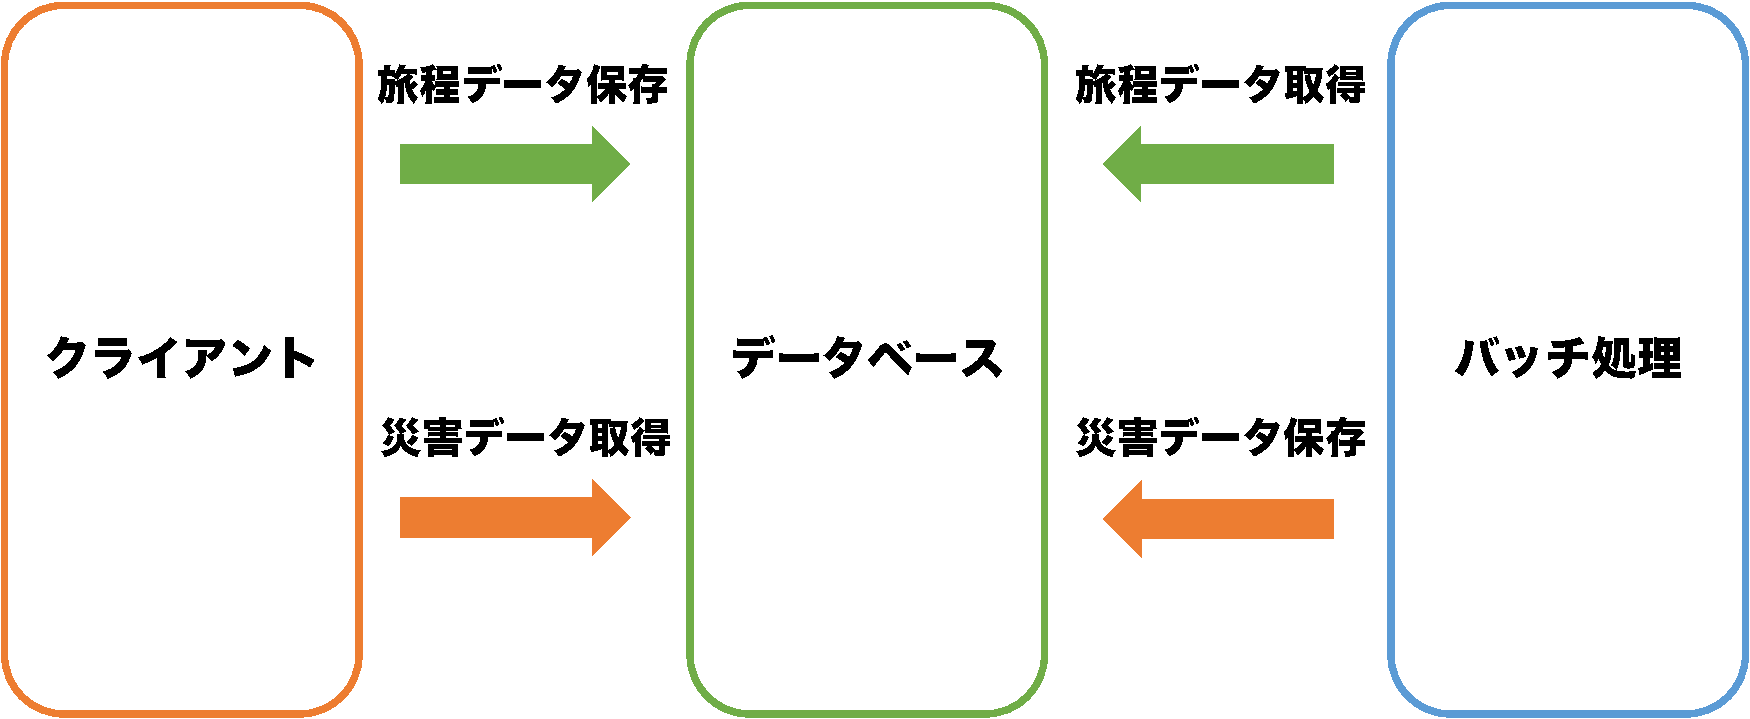
\includegraphics[height=6cm]{figure31.pdf}
  %\vspace{-3mm}
  \caption{システムの全体概要図}
  \label{fig:system_summary}
  %\vspace{2mm}
\end{figure}

\subsection{クライアント部}
クライアント部はこのシステムにおけるユーザインタフェースの役割を持つ.
旅程データの入力機能と注意情報を提供する機能がある.
具体的にはモバイルアプリケーションとして開発した.

\subsubsection{旅程データの入力機能}
ユーザはまず旅程のタイトルと期間を入力し,旅程パッケージを作成する.
旅程パッケージとは旅程データを1つにまとめたものである.
旅程データには,場所データと交通機関のデータの2種類が存在する.ユーザはこの2種類のデータで旅程を構築する.
ユーザは訪れる予定の場所や利用する予定の交通機関の位置情報を,予定時刻とともに入力インタフェースを通して入力する.
位置情報は両方の種類においても都道府県と市区町村名の名称である.
インタフェースは旅程パッケージごとに入力されたデータをデータベースへ保存する.
保存する際には旅程パッケージにクライアントIDを付与する.

\subsubsection{注意情報提供機能}
第1章で定義したストック情報とフロー情報をユーザに提供する.
旅程データの入力機能にて事前に入力した旅程データのうち,災害の影響を受けると判断された旅程データを表示する.
その際に影響を受ける災害の種類と可能性の確率を提供する.
さらに,ユーザに対して災害の種類ごとにその現象と対処法についての情報を提供する.
また,影響を受ける旅程データが交通機関である場合,災害の可能性を交通機関が運休する可能性として情報を提供する.
その際に,運休によって起こる現象についての情報を提供する.

\subsection{データベース部}
データベース部はこのシステムにおけるデータを管理する役割を持つ.
データを保存する機能とデータを提供する機能がある.
具体的にはクラウドデータベースを用いている.

\subsubsection{データ保存機能}
ユーザがクライアント部で入力した旅程データを旅程パッケージごとに保管する.
また,バッチ処理部で旅程データと紐付けられた注意情報も保管する.

\subsubsection{データ提供機能}
クライアント部の要求には,旅程パッケージに付与されているクライアントIDを条件にデータを提供する.
バッチ処理部の要求には,旅程データの予定時刻を条件にデータを提供する.

\subsection{バッチ処理部}
バッチ処理部は,旅程データが災害の影響を受けるか監視する役割を持つ.
気象庁が定期的に公表する,注意情報を取得して,ユーザがクライアント部で入力した旅程データと照合する.
災害の影響を受ける旅程データがあれば注意情報と旅程データを紐づけてデータベースに保存する.
旅程データを作成したクラアントに通知する指示を出す.
具体的にはPythonのプログラムを作成して,定期事項している.

\subsubsection{気象庁から注意情報の取得}
注意情報とは災害の影響を受ける可能性と予定時刻,発表地域で構成される情報である.
この情報は気象庁から定期的にWeb上で発表されている.
その時刻に合わせてバッチ処理が実行され,注意情報を取得する.

\subsubsection{旅程データの取得}
注意情報の予定時刻と重なる旅程データを検索する.
データベース部から旅程データを取得する.

\subsubsection{注意情報と旅程データを照合}
注意情報の予報時刻に当てはまる旅程データを抽出した後,旅程データの場所情報をもとに,注意情報を関連付けて保存するか判断する.
注意情報の発表地区は気象庁が独自に定めている,各都道府県の市区町村のまとまりである.
注意情報に災害の予測が記載されている場合,旅程データの位置情報から発表地区に属するデータを抽出し,注意情報を旅程データと紐付ける.
災害の影響を受けると判断された旅程データはデータベースに保存する.
もし注意情報に災害の予測が記載されてなければ何もしない.


\subsubsection{クライアント部へ通知指示}
災害の影響を受けると判断された旅程データを作成したクライアントに通知を送信するよう指示を出す.
しかし,評価実験をするにあたって評価指標とは関連がない機能であったことと,コスト削減のため本研究ではクライアント部からの通知機能を実装した.

\subsection{処理の流れ}
システムの処理の流れについて述べる.
図 \ref{fig:activity}にアクティビティを示す.

\begin{quote}
  \begin{enumerate}
    \item 旅程データの入力(クライアント部)
    \item 旅程データの保存(データベース部)
    \item 気象庁から注意情報の取得(バッチ処理部)
    \item 旅程データの取得(バッチ処理部)
    \item 旅程データの提供(データベース部)
    \item 注意情報と旅程データを照合(バッチ処理部)
    \item 注意情報の保存(データベース部)
    \item クライアント部へ通知指示(バッチ処理部)
    \item 通知(クライアント部)
    \item 注意情報の提供(データベース部)
    \item 注意情報提供(クライアント部)
  \end{enumerate}
\end{quote}

\begin{figure}[H]
  \centering
  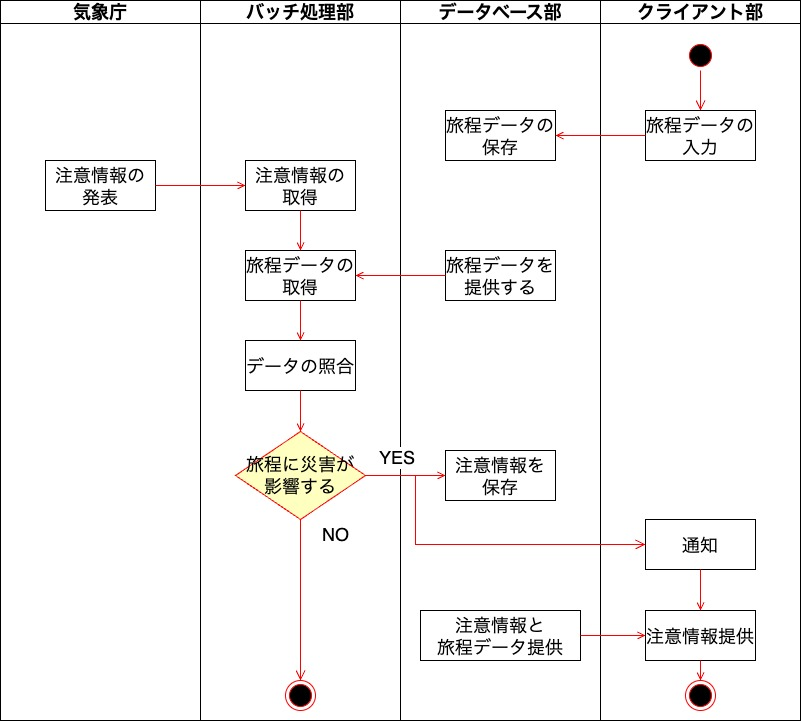
\includegraphics[height=10cm]{figure32.jpg}
  %\vspace{-3mm}
  \caption{システムのアクティビティ図}
  \label{fig:activity}
  %\vspace{2mm}
\end{figure}
\section{ファイル構成}
配布したフォルダには様々なファイルが同梱されているが,拡張子が「tex,bib,cls,bat」であるファイルが重要である.

拡張子が「tex」ファイルは,本文を記載するファイルである.
本文中には,\LaTeX の命令をマークアップしていく.

拡張子が「bib」ファイルは,参考文献を記載するファイルである.
\BibTeX の命令でマークアップしていく.
このファイルを \LaTeX 側から呼び出し,参照したり番号を割り振ったりする.

拡張子が「cls」ファイルは,設定事項を記載するファイルである.
基本的に,この拡張子のファイルは変更する必要は無い.

拡張子が「bat」ファイルは,\LaTeX のソースファイルから,PDFファイルを作成するまでの一連の命令を実行するバッチファイルである.
\LaTeX において標準的には,本バッチファイル内の命令は各自で順に実行するのだが,煩雑である.
宮治が作成した(というほどのものではないが)本バッチファイルを実行すれば,その中の命令は意識する必要はない.
今回配布のバッチファイルは Macintosh と Windowsで別のものを利用する.

主要なファイルの説明を 表\ref{table:files2}に記載する.
\begin{table}[H]
\centering
\caption{スタイルパッケージ内のファイル説明}
\vspace{-2mm}
{\footnotesize
\begin{tabular}{|l|l|l|}
\hline
ファイル名 & 内容 & 注意\\\hline\hline
settings.tex & 論文の必要事項設定ファイル & 必ず編集\\\hline
main.tex & 大元のファイル & 読み込むファイルなどを設定\\\hline
main.dvi & できたファイル & \\\hline
main.pdf & pdfファイル & dvi ファイルを元に作成\\\hline
myjlab.sty & 宮治研用スタイルファイル & 変更不要\\\hline
myjlabthesisstyle.sty & 各種スタイルファイルを読み込む & 必要に応じて追加\\\hline
abstract.tex & 要旨を記述 & 章や節の命令は入れずに文章を入力\\\hline
thanks.tex & 謝辞を記述 & 章や節の命令は入れずに文章を入力\\\hline
chap1.tex & 第1章を記述 & \\\hline
chap2.tex & 第2章を記述 & \\\hline
sec21.tex, sec22.tex など& 2章1節と2節のファイル & chap2.texが大きくなったのでファイルを分割\\\hline
chap3.tex & 第3章を記述 & 注:3章内のファイルも節毎にファイルを分割\\\hline
chap4から6.tex & 4章から6章のファイル & 配布無し,各自で作成し,main.tex修正\\\hline
appendixa.tex & 付録Aを記述 & \\\hline
appendixb.tex & 付録Bのファイル & 配布無し,各自で作成し,main.tex修正\\\hline
myrefs.bib & 参考文献情報ファイル & 記述方法が特殊\\\hline
mklatex.bat & Macintosh用の実行バッチファイル & 命令を憶えずとも,main.tex⇒main.pdf\\\hline
winmklatex.bat & Windows用の実行バッチファイル & 命令を憶えずとも,
main.tex⇒main.pdf\\\hline
dmklatex.bat & Docker用の実行バッチファイル & 命令を憶えずとも,
main.tex⇒main.pdf\\\hline
\end{tabular}
}
\label{table:files2}
\end{table}

これらのファイルの変更方法,記入方法を以降で解説する.
\section{settings.tex: 論文の設定情報を記述}
settings.tex には,各自の個人情報や論文のタイトルなどを設定する.

\subsection{各自の情報設定}
各自の情報を設定する際には,サブタイトルの有り/無しで設定事項が異なることに注意をする必要がある.
それぞれの方法について以下に記述する.
また,これらの作業が終わった時点で,本配布スタイルパッケージの動作確認をすることをおすすめする.

\subsubsection{サブタイトル有りの場合}
配布したファイルは,サブタイトルがある場合のサンプルになっている.
各自の 年度,提出年月,学籍番号,氏名,タイトル,サブタイトルを所定の命令内に記入する.
\begin{breakbox}
{\small
%footnotesize
\begin{verbatim}
\nendo{2013年度}
\teisyutsu{2014年~~1月}
\snum{15387019}
\jname{宮治 裕}
\thesistitle{宮治研における論文作成について} %タイトルを記入
\thesissubtitle{\LaTeX の利用} %サブタイトルを記入 ない場合はコメントアウト
\SUBTtrue %サブタイトル有りの場合 ない場合は,コメントアウト
%\SUBTfalse %サブタイトル無しの場合 有る場合は,コメントアウト
\end{verbatim}
}
\end{breakbox}

\subsubsection{サブタイトル無しの場合}
サブタイトル有りの場合と比較して2箇所の変更が必要である.
サブタイトルを記入する命令の先頭部分に \% 記号を入れ,コメントアウト状態にする.

\begin{breakbox}
{\small
\begin{verbatim}
%\thesissubtitle{\LaTeX の利用} %サブタイトルを記入 無い場合は,コメントアウト
\end{verbatim}
}
\end{breakbox}
もう一つは,その直下の2行
\begin{breakbox}
{\small
\begin{verbatim}
\SUBTtrue %サブタイトル有りの場合 無い場合は,コメントアウト
%\SUBTfalse %サブタイトル無しの場合 有る場合は,コメントアウト
\end{verbatim}
}
\end{breakbox}
以下の様に変更する.
\begin{breakbox}
{\small
\begin{verbatim}
%\SUBTtrue %サブタイトル有りの場合 無い場合は,コメントアウト
\SUBTfalse %サブタイトル無しの場合 有る場合は,コメントアウト
\end{verbatim}
}
\end{breakbox}

以上の設定で,表紙と各ページのヘッダ・フッタの情報が自動的に設定され,書式が整えられる.
\begin{boxnote}
\LaTeX では 「\verb+%+」はコメントを意味し,この記号から改行コードまでをコメントアウト状態として処理する.
\end{boxnote}
であることに注意すること.

\subsection{スタイルパッケージの動作確認}
サブタイトルの有り/無しに応じて適切に設定ができた段階で,一度各自の環境下でスタイルパッケージが正常動作することを確認して欲しい.
正常動作した場合には,本ファイルとほぼ同様の中身で,表紙と各ページのヘッダとフッタが各自の設定した情報が記載されたPDFファイルが出来上がるはずである.

まず,Macintoshの場合について記す.
各自のホームディレクトリ中のDropboxフォルダ内に,本スタイルパッケージが展開されている場合を前提として記述する.
\begin{enumerate}
\item まず,ターミナルを開く
\item 以下のコマンドを入力し,スタイルパッケージのあるフォルダに移動
\footnote{ここで \verb+$+記号は,コマンドプロンプトを表すため,入力しないように.}
\begin{screen}
{\small
\begin{verbatim}
 $ cd ~/Dropbox/Thesis
\end{verbatim}
}
\end{screen}

\item そこで,バッチファイル \verb+mklatex.bat+ を実行
\begin{screen}
{\small
\begin{verbatim}
 $ ./mklatex.bat
\end{verbatim}
}
\end{screen}

\item main.pdfファイルが作成され,プレビュー画面が自動で表示される
\item[\textbf{注}] mklatex.bat が実行できないというようなエラーが出た場合には,最初の一回だけ(次回から不要)以下の命令を入力する
\begin{screen}
{\small
\begin{verbatim}
 $ chmod 755 ./mklatex.bat
\end{verbatim}
}
\end{screen}
\end{enumerate}

正常動作しなかった場合には,出来上がった main.log ファイルを宮治に送付して欲しい.

Windowsの場合には,コマンドプロンプトを開き,目的のフォルダに移動し,バッチファイル(winmklatex.bat)を起動する.
\begin{screen}
{\small
\begin{verbatim}
 $ cd c:\My Documents\Dropbox\Thesis
 $ winmklatex.bat
\end{verbatim}
}
\end{screen}
main.pdfファイルができるので,エクスプローラからファイルをダブルクリックしてAcrobat Reader にて確認して欲しい.

\section{使用方法}

本研究のシステムの使用方法を述べる.使用手順は以下の通りである.

\begin{quote}
  \begin{enumerate}
    \item アプリを起動する
    \item 旅程パッケージを作成する
    \item 旅程データを作成する
    \item 通知を受け取る
    \item 災害注意予報を確認する
    \item ストック情報を確認する
  \end{enumerate}
\end{quote}

\subsection{アプリを起動する}
アプリを利用するのに,旅行計画の作成が必要であるため,機能メニューの旅行計画をタップする.
ホーム画面はアプリを立ち上げたとき,最初に表示される画面である.
この画面ではアプリの概要について説明が閲覧できる.
この画面から予報についての画面と旅程パッケージの作成画面に遷移できる.

\begin{figure}[H]
  \centering
  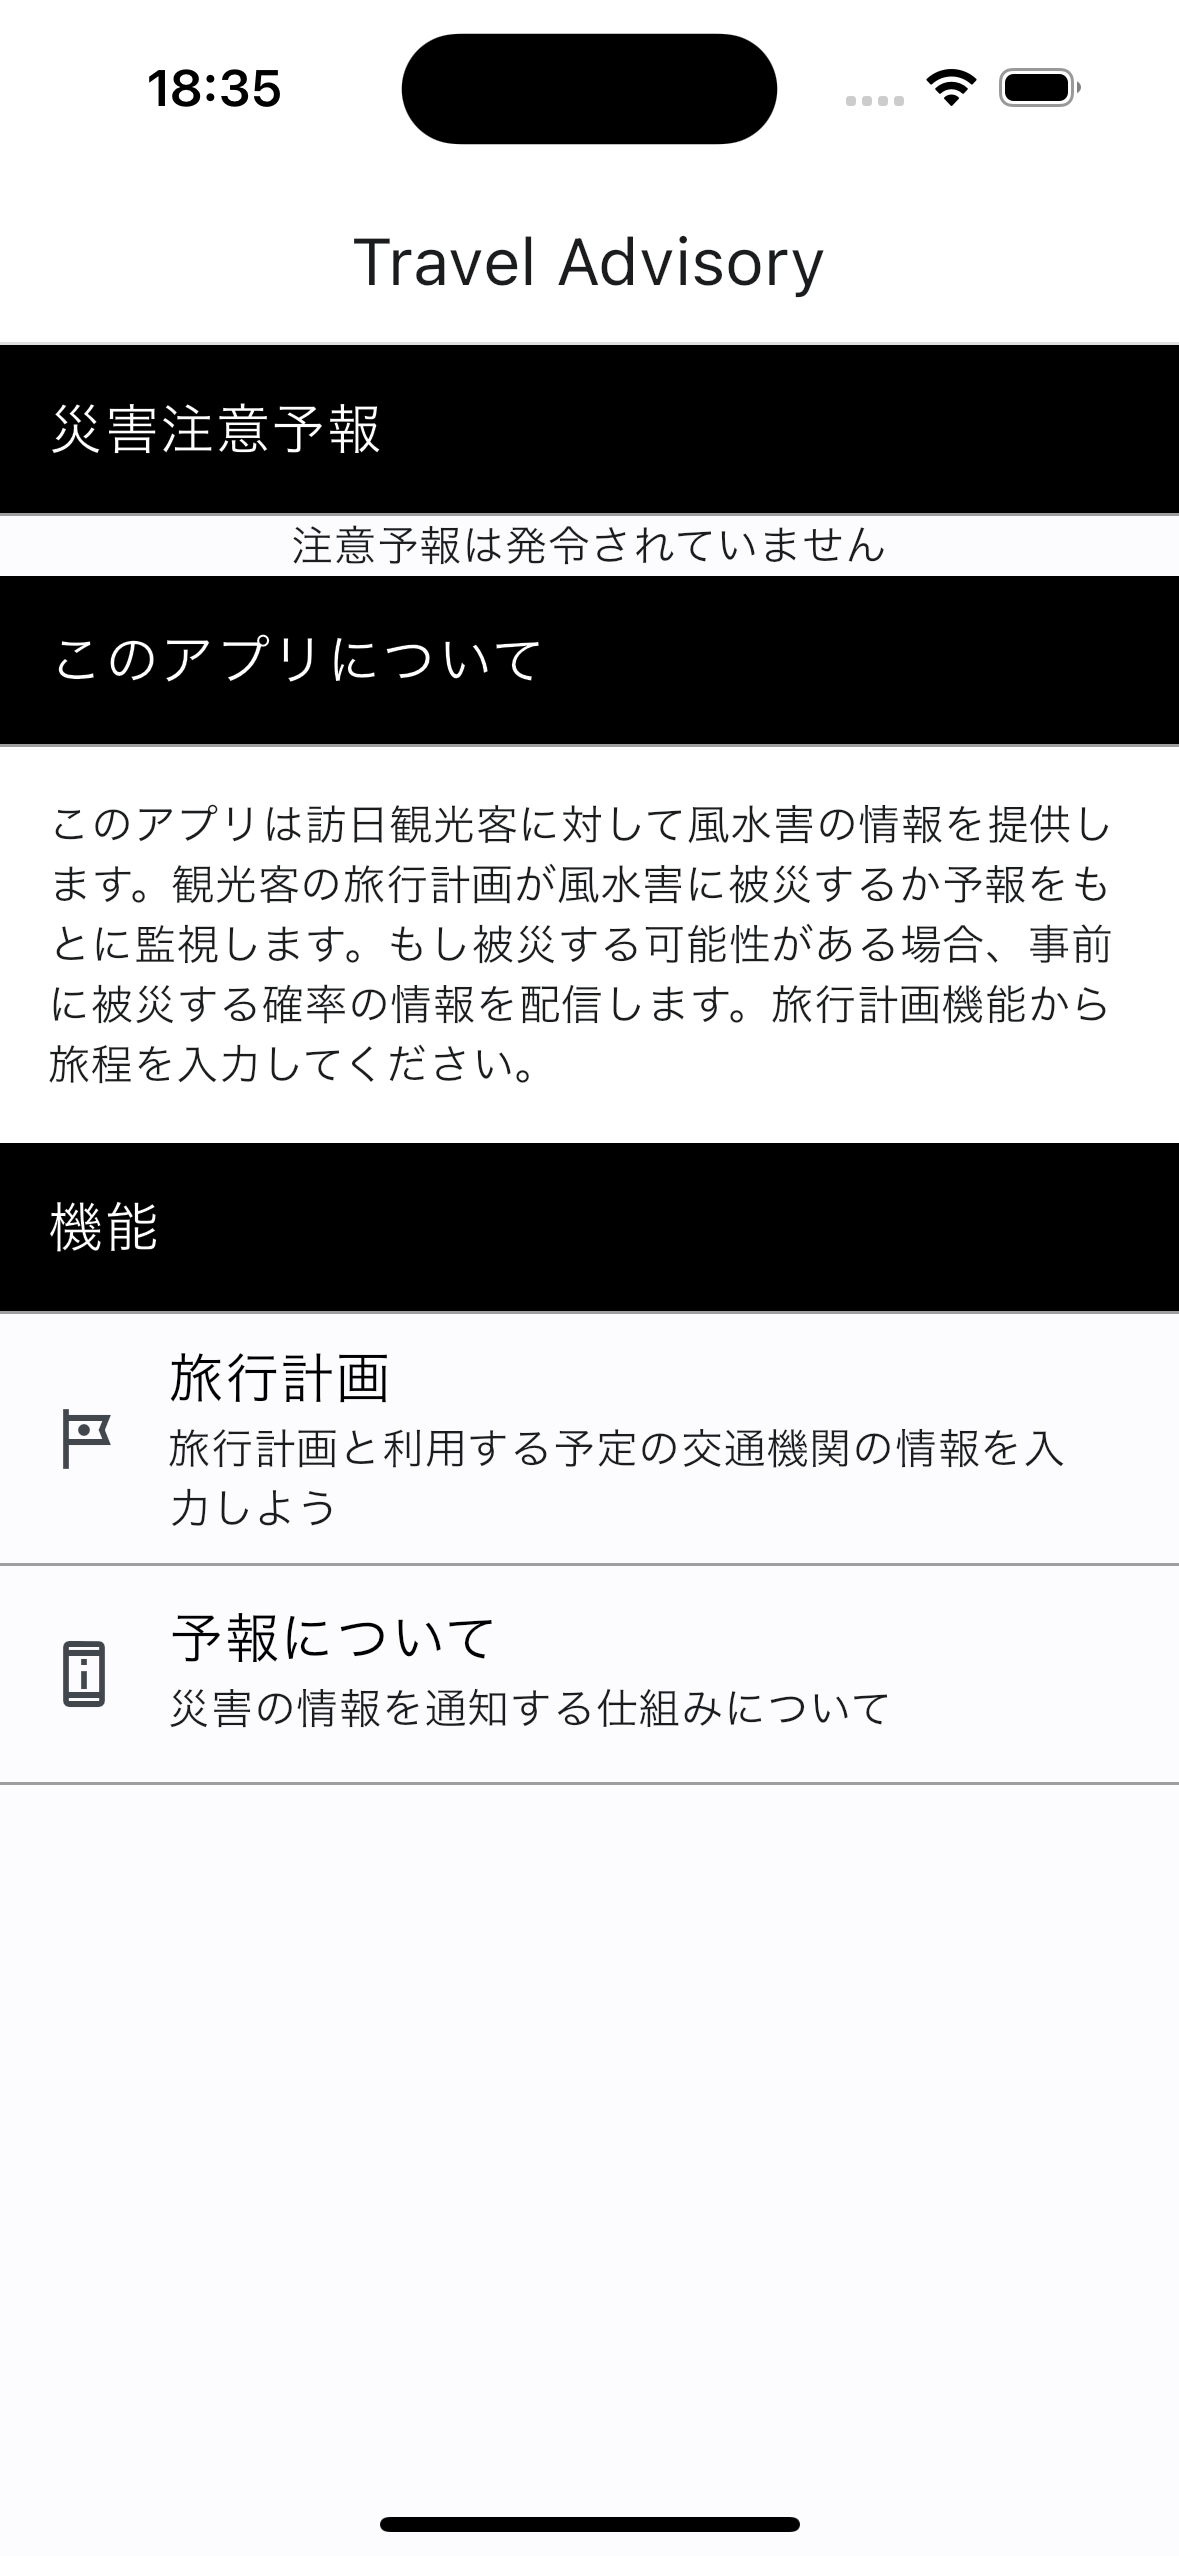
\includegraphics[height=10cm]{./fig/normal_home_screen.png}
  %\vspace{-3mm}
  \caption{通常時のホーム画面}
  \label{fig:normal_home_screen}
  %\vspace{2mm}
\end{figure}

% \subsection{予報についての画面}
% 予報についての画面はアプリケーションが提供する災害注意予報について説明している画面である。
% アプリでの予報の表示の仕方や、気象庁防災情報XMLについて簡単に説明している。

% \begin{figure}[H]
%   \centering
%   \includegraphics[height=8cm]{./fig/forcast_screen_1.png}
%   %\vspace{-3mm}
%   \caption{予報についての画面の図1}
%   \label{fig:forecast_screen_1}
%   %\vspace{2mm}
% \end{figure}

% \begin{figure}[H]
%   \centering
%   \includegraphics[height=8cm]{./fig/forcast_screen_2.png}
%   %\vspace{-3mm}
%   \caption{予報についての画面の図2}
%   \label{fig:forecast_screen_2}
%   %\vspace{2mm}
% \end{figure}

\subsection {旅程パッケージを作成する}
旅程データを作成するために旅程パッケージを作成する.
旅程パッケージ画面は作成した旅程パッケージの一覧と旅行パッケージの作成機能を提供している画面である.
旅行パッケージは右下の計画の作成ボタンをタップすると旅行パッケージ作成画面に遷移して作成できる.
旅行パッケージの一覧からパッケージをタップすると,旅程データ画面に遷移する.

\begin{figure}[H]
  \begin{minipage}[b]{0.45\linewidth}
    \centering
    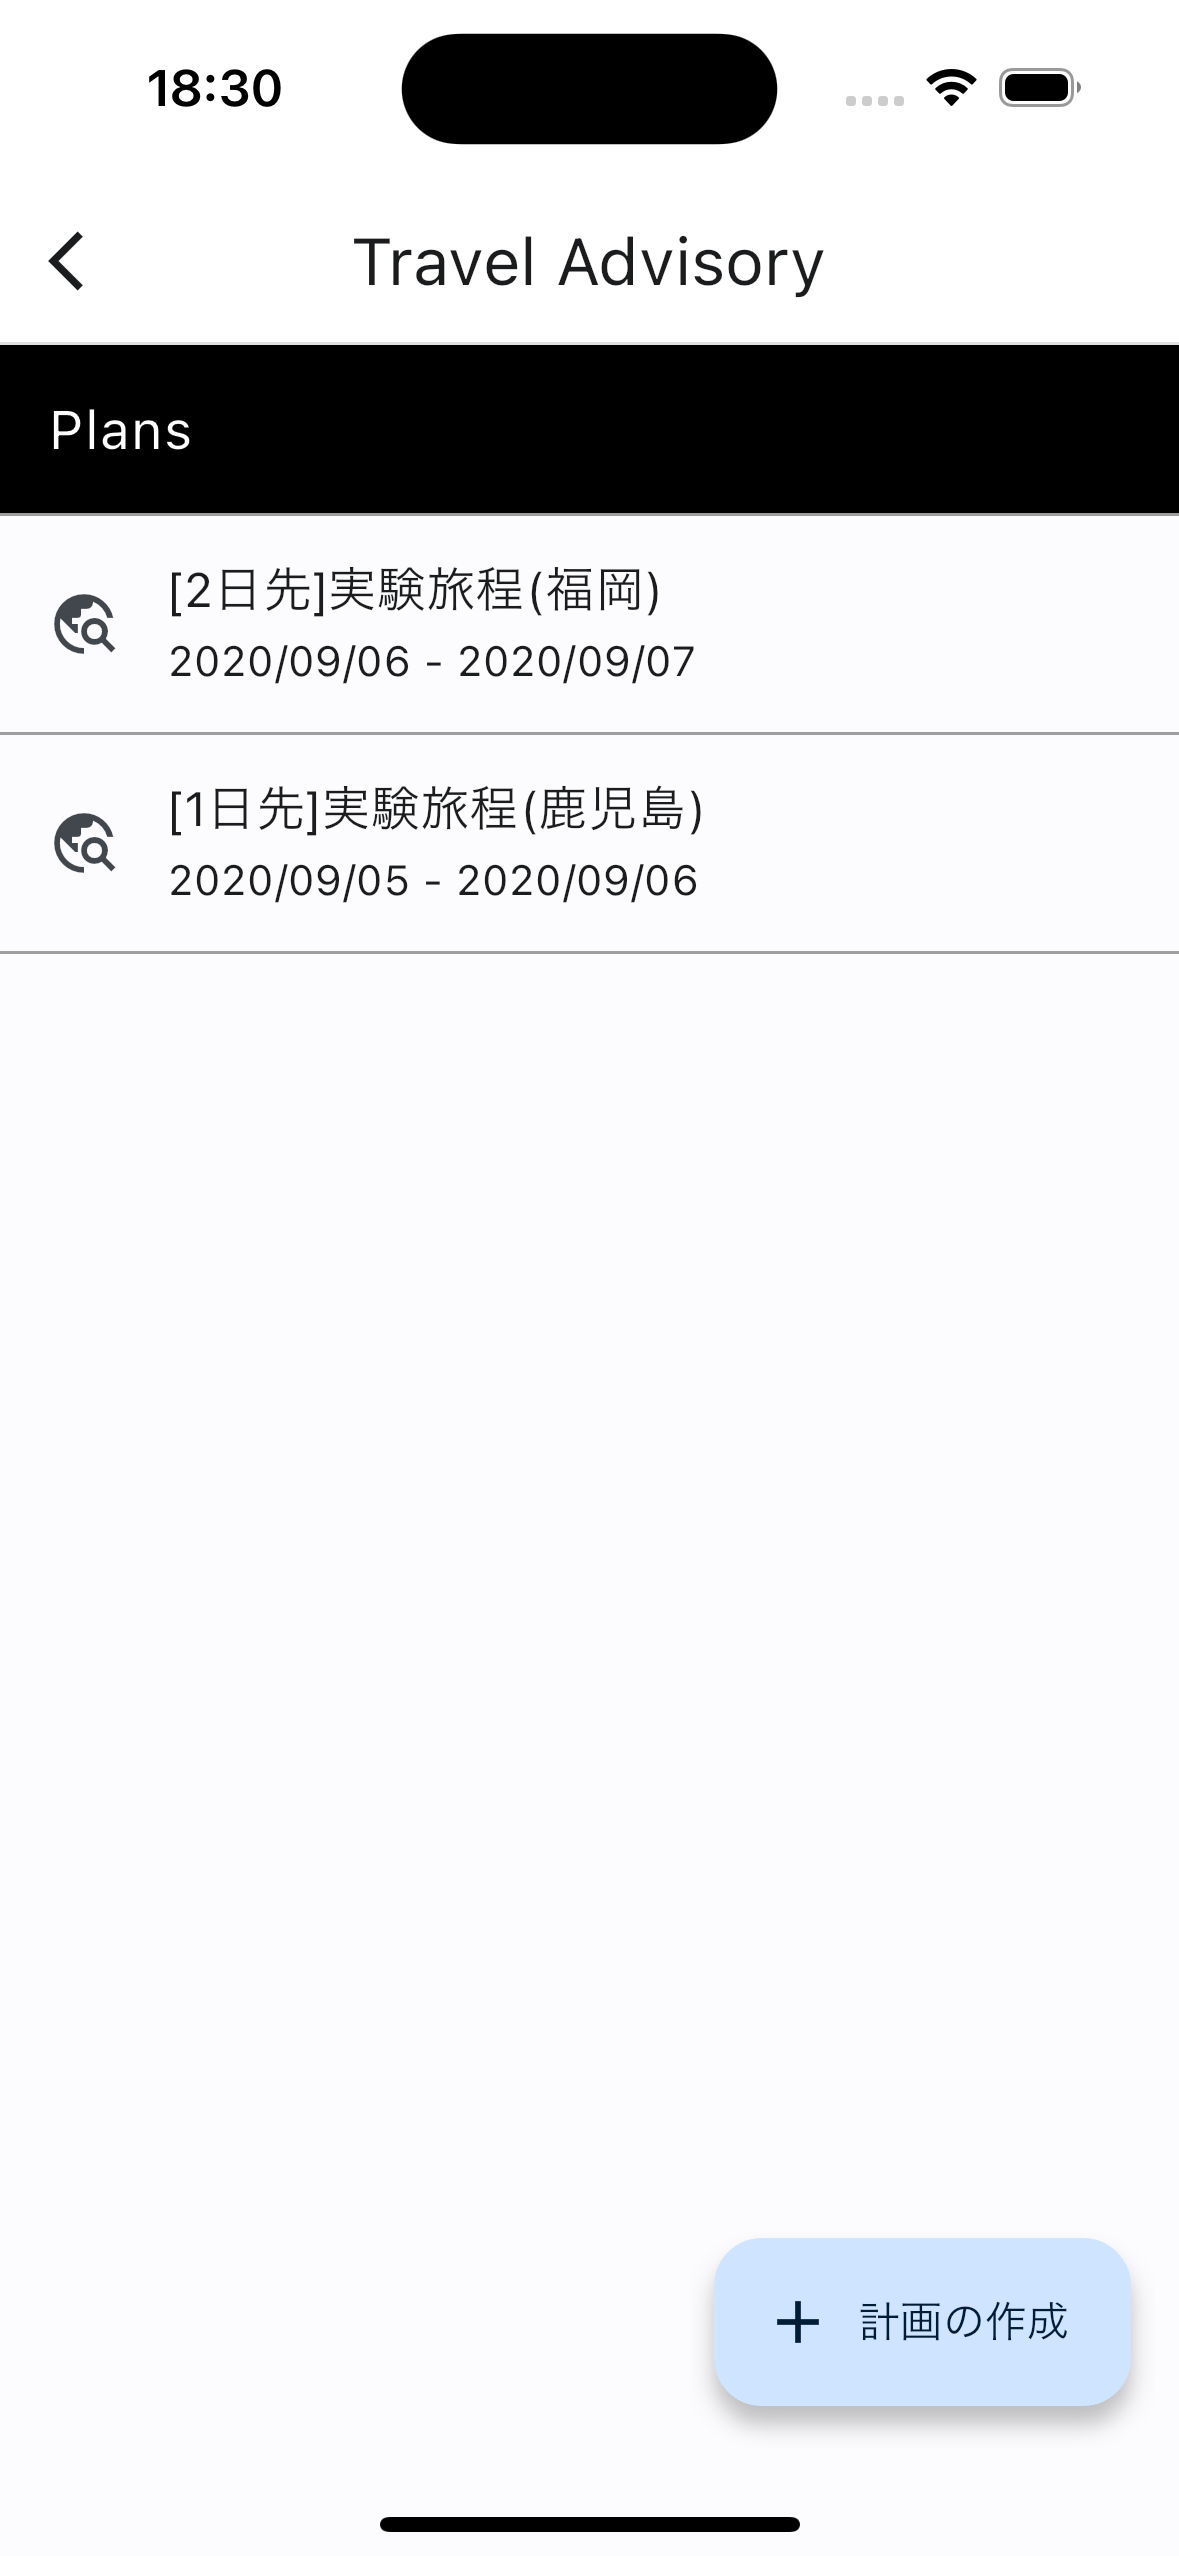
\includegraphics[height=10cm]{./fig/travel_pack_list.png}
    %\vspace{-3mm}
    \caption{旅程パッケージ画面}
    \label{fig:travel_pack_list}
    %\vspace{2mm}
  \end{minipage}
  \begin{minipage}[b]{0.45\linewidth}
    \centering
    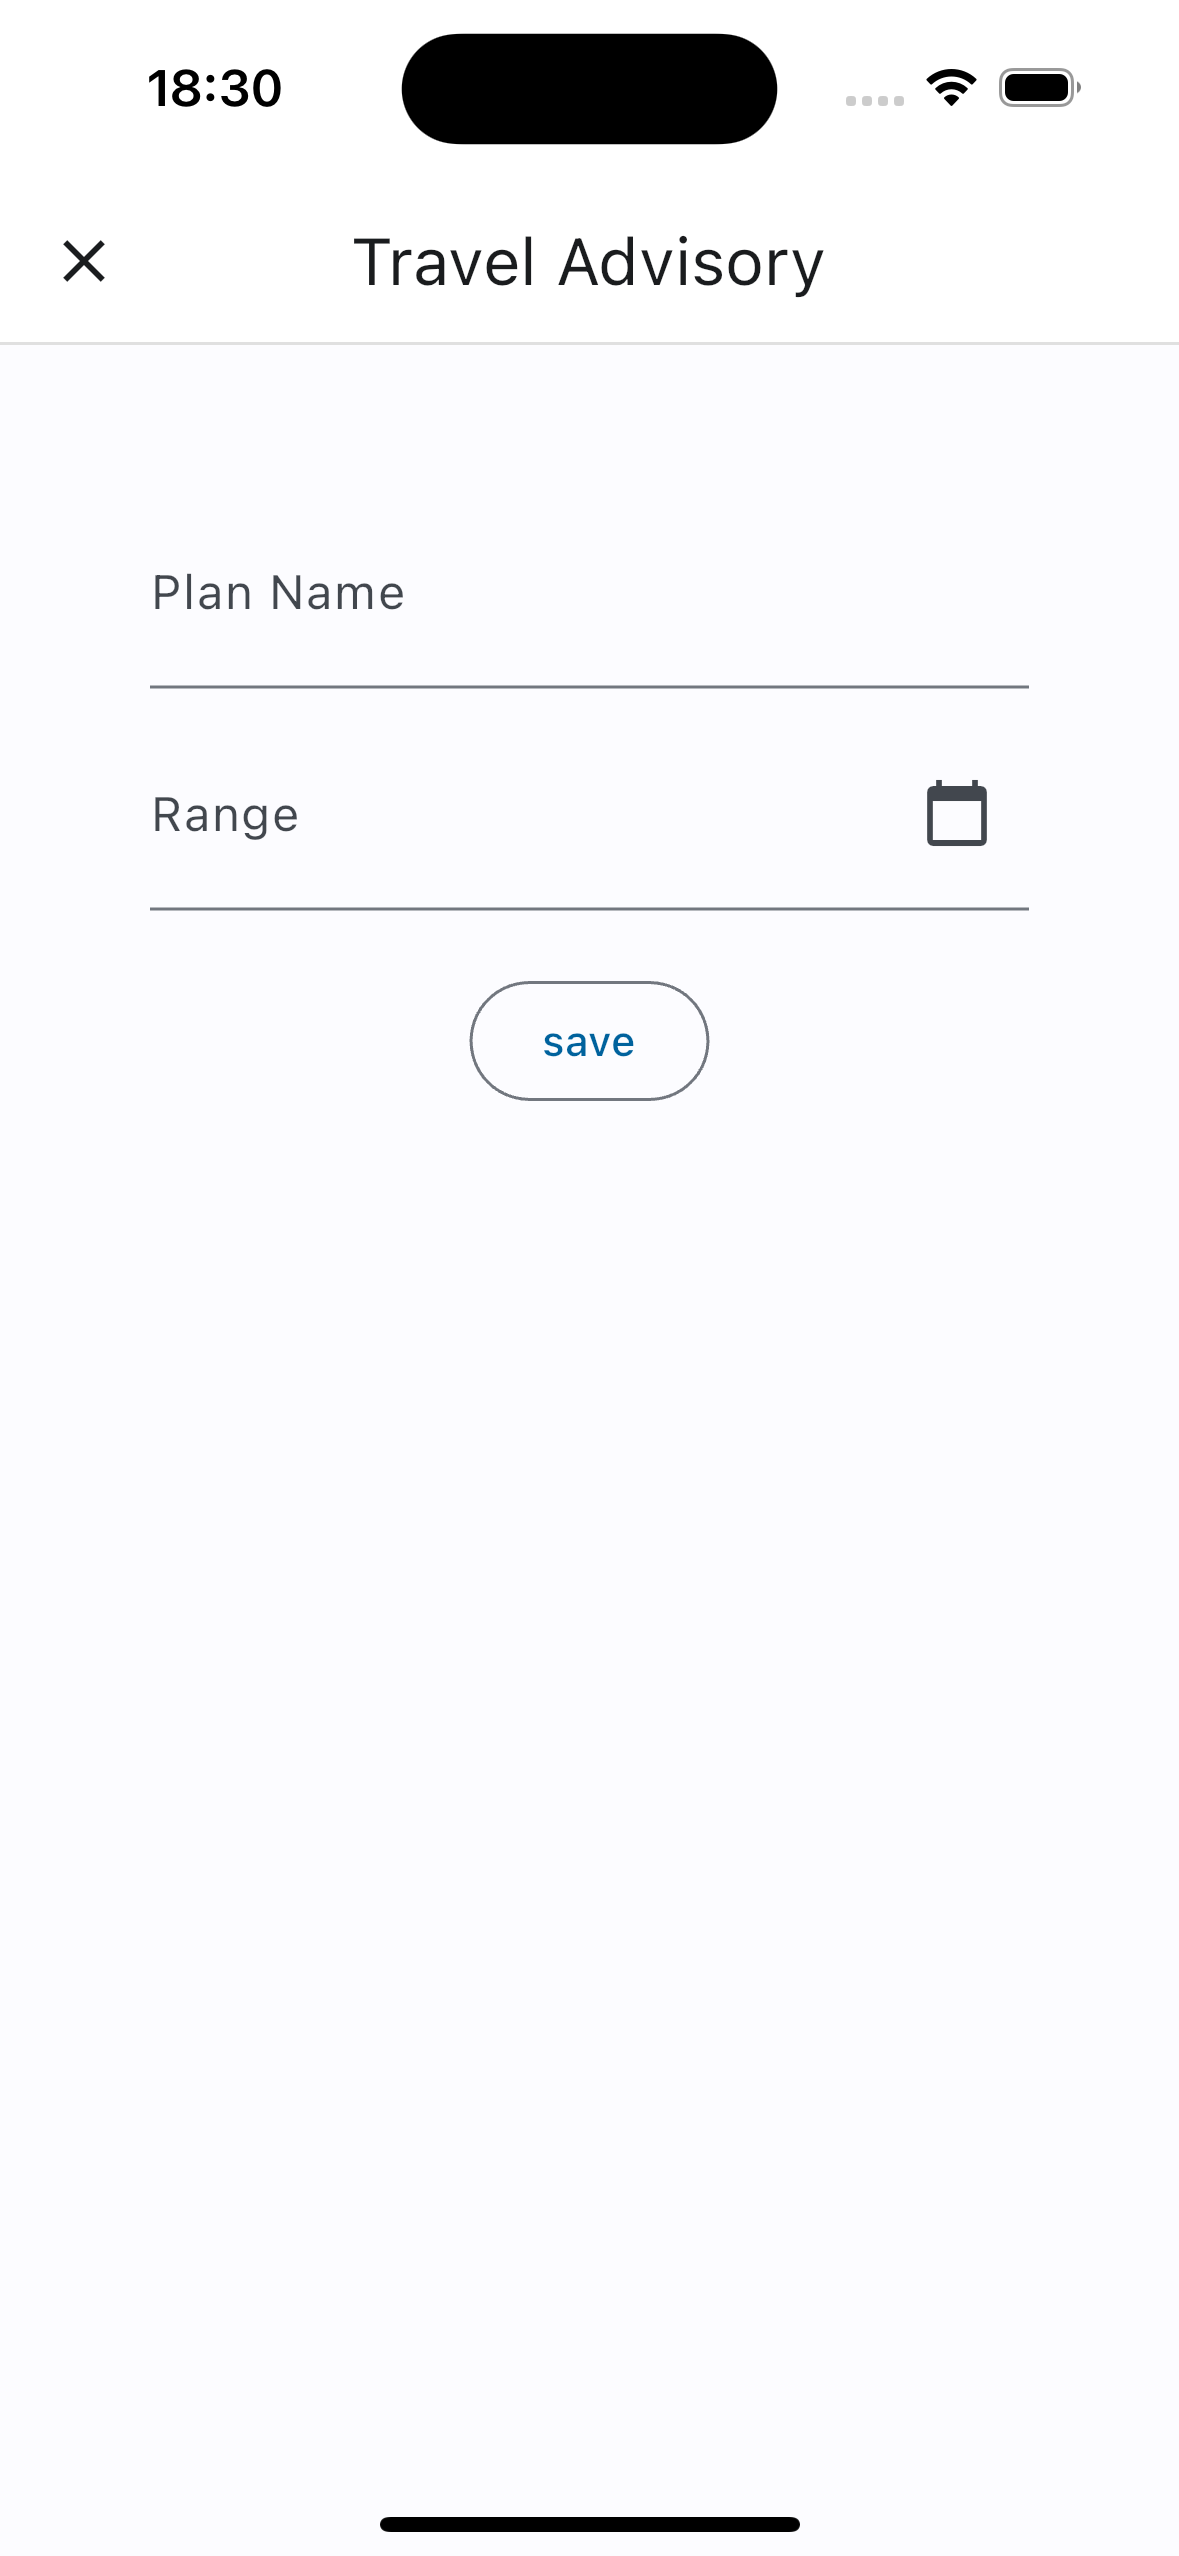
\includegraphics[height=10cm]{./fig/travel_pack_create.png}
    %\vspace{-3mm}
    \caption{旅程パッケージ作成画面}
    \label{fig:travel_pack_create}
    %\vspace{2mm}
  \end{minipage}
\end{figure}

\subsection {旅程データを作成する}
旅程パッケージに旅程データを作成し,登録する.
旅程データ画面は日付ごとに作成した旅程データの一覧と場所・交通データの作成機能を提供している画面である.
下部のAdd Spotボタンをタップすると場所データの作成が,Add Transportationボタンをタップすると交通データの作成画面に遷移する.

\begin{figure}[H]
  \centering
  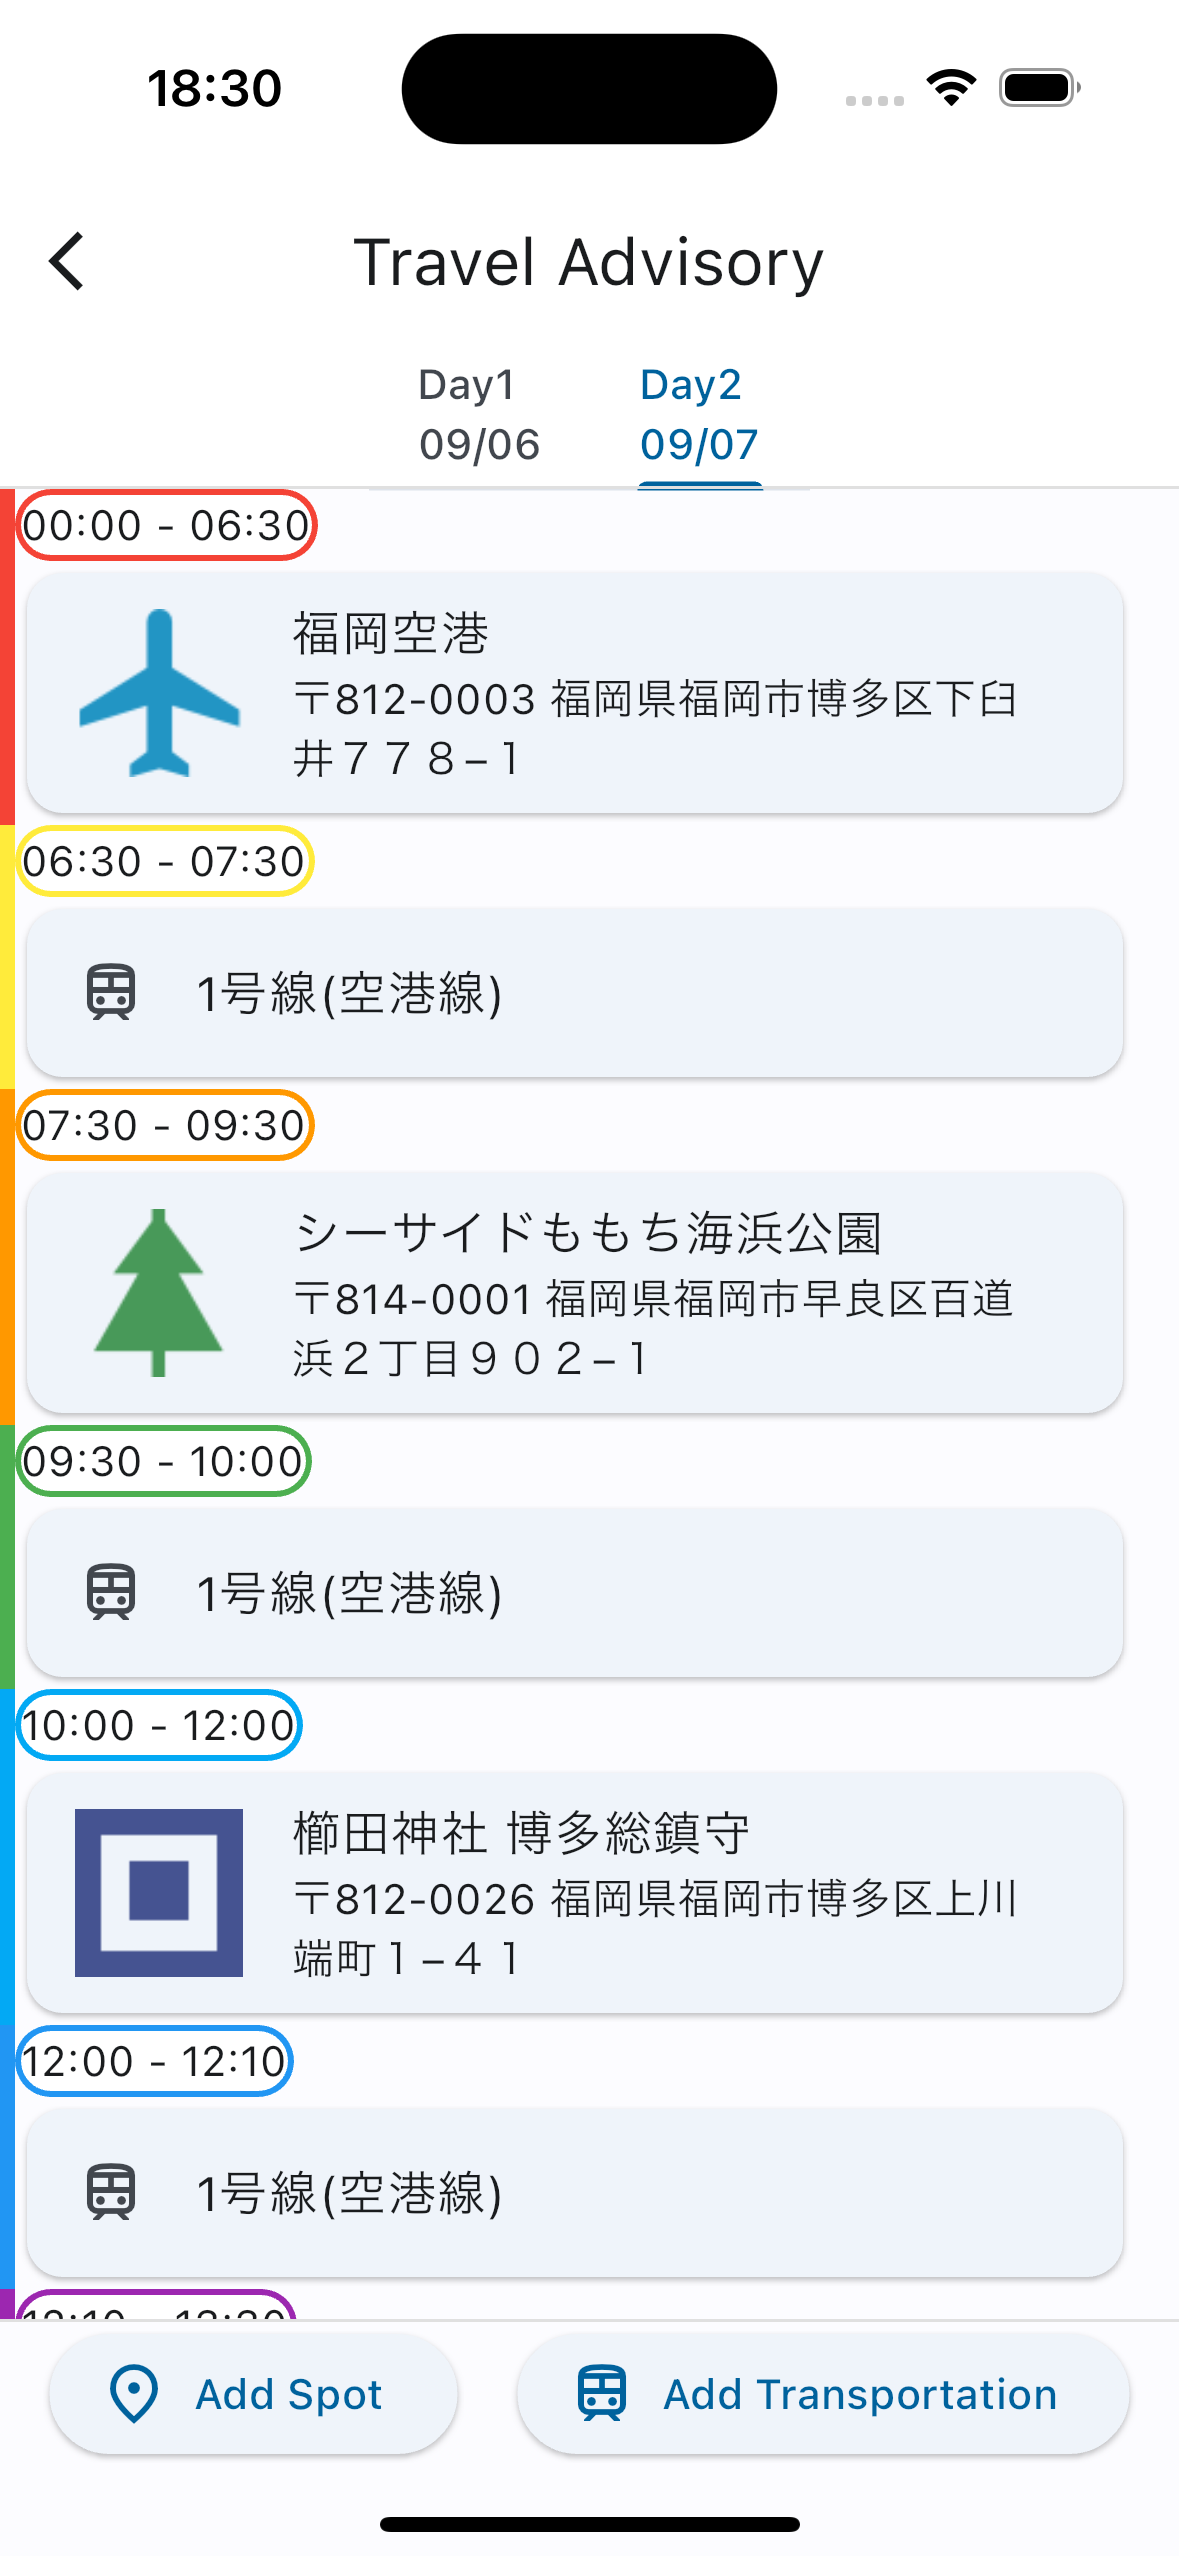
\includegraphics[height=10cm]{./fig/travel_data_list.png}
  %\vspace{-3mm}
  \caption{旅程データ画面}
  \label{fig:travel_data_list}
  %\vspace{2mm}
\end{figure}

\subsubsection {場所データの作成}
場所データを作成する.
訪れる予定の場所を検索する機能とその時刻を入力する機能を提供している画面である.
検索機能はGoogle Map Apiを利用している.
検索すると場所の候補が複数表示されるので,1つを選択してSaveボタンを押す.

\begin{figure}[H]
  \centering
  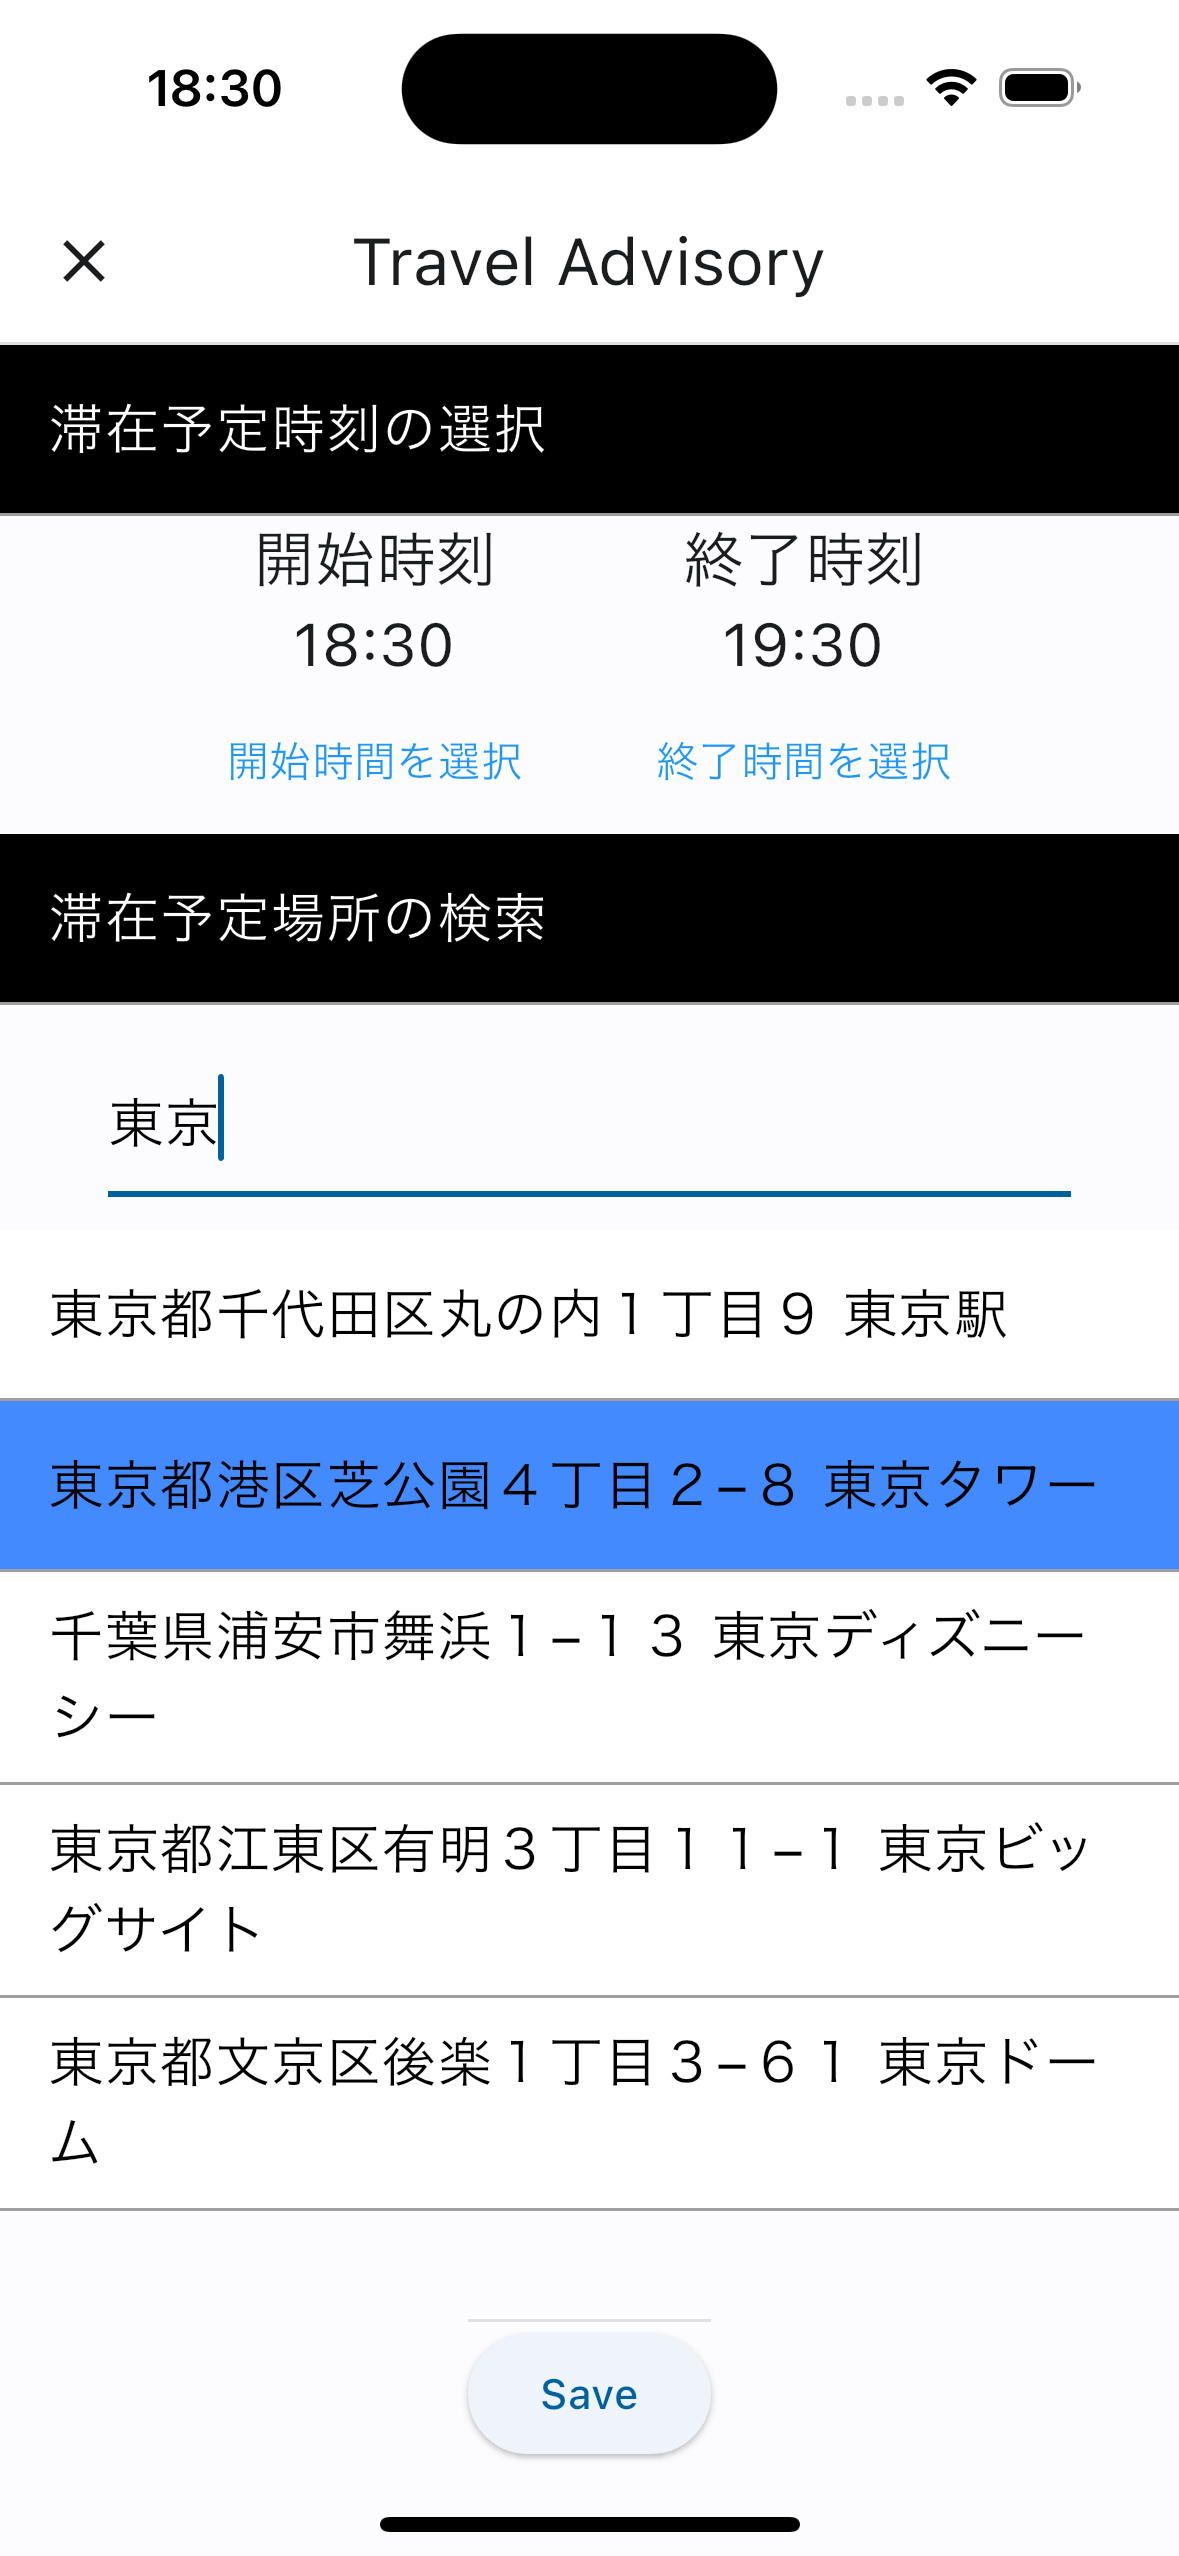
\includegraphics[height=10cm]{./fig/spot_data_save.png}
  %\vspace{-3mm}
  \caption{場所データの作成画面}
  \label{fig:spot_data_save}
  %\vspace{2mm}
\end{figure}

\subsubsection {交通機関データの作成}
交通データを作成する.
利用する予定の鉄道の路線を検索する機能を提供する.
路線を選択した後,路線に属する駅の一覧が表示される.
自分が利用する予定の駅を1つ以上選択し,時刻とともにデータを保存する.

\begin{figure}[H]
  \begin{minipage}[b]{0.45\linewidth}
    \centering
    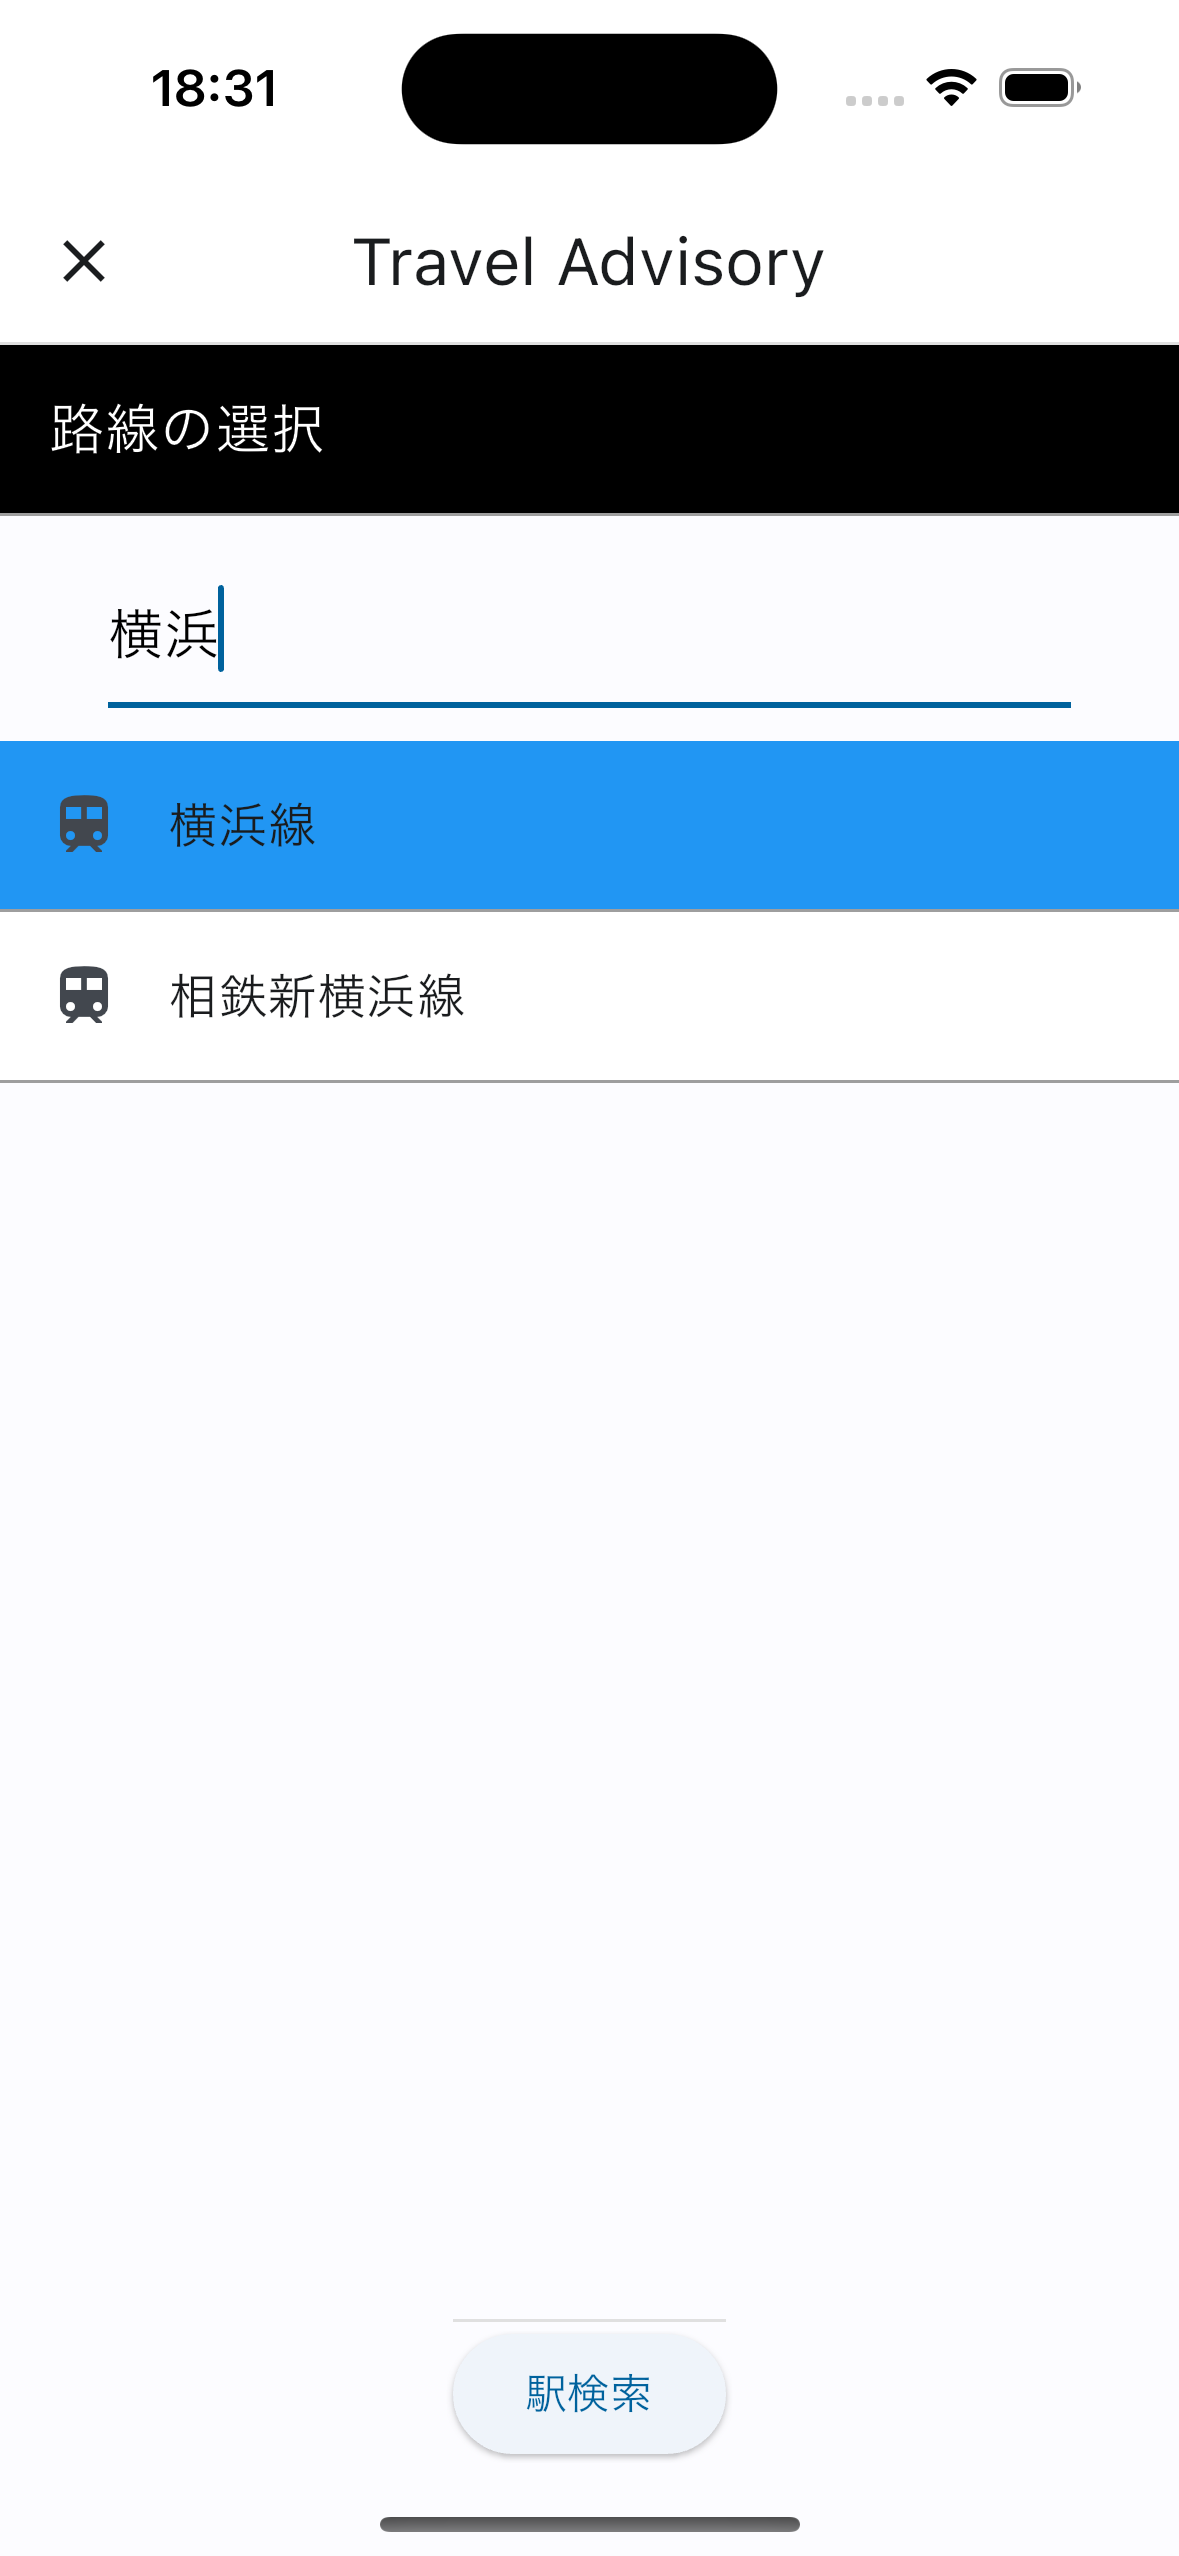
\includegraphics[height=10cm]{./fig/railway_search.png}
    %\vspace{-3mm}
    \caption{鉄道の路線を検索する画面}
    \label{fig:railway_search}
    %\vspace{2mm}
  \end{minipage}
  \begin{minipage}[b]{0.45\linewidth}
    \centering
    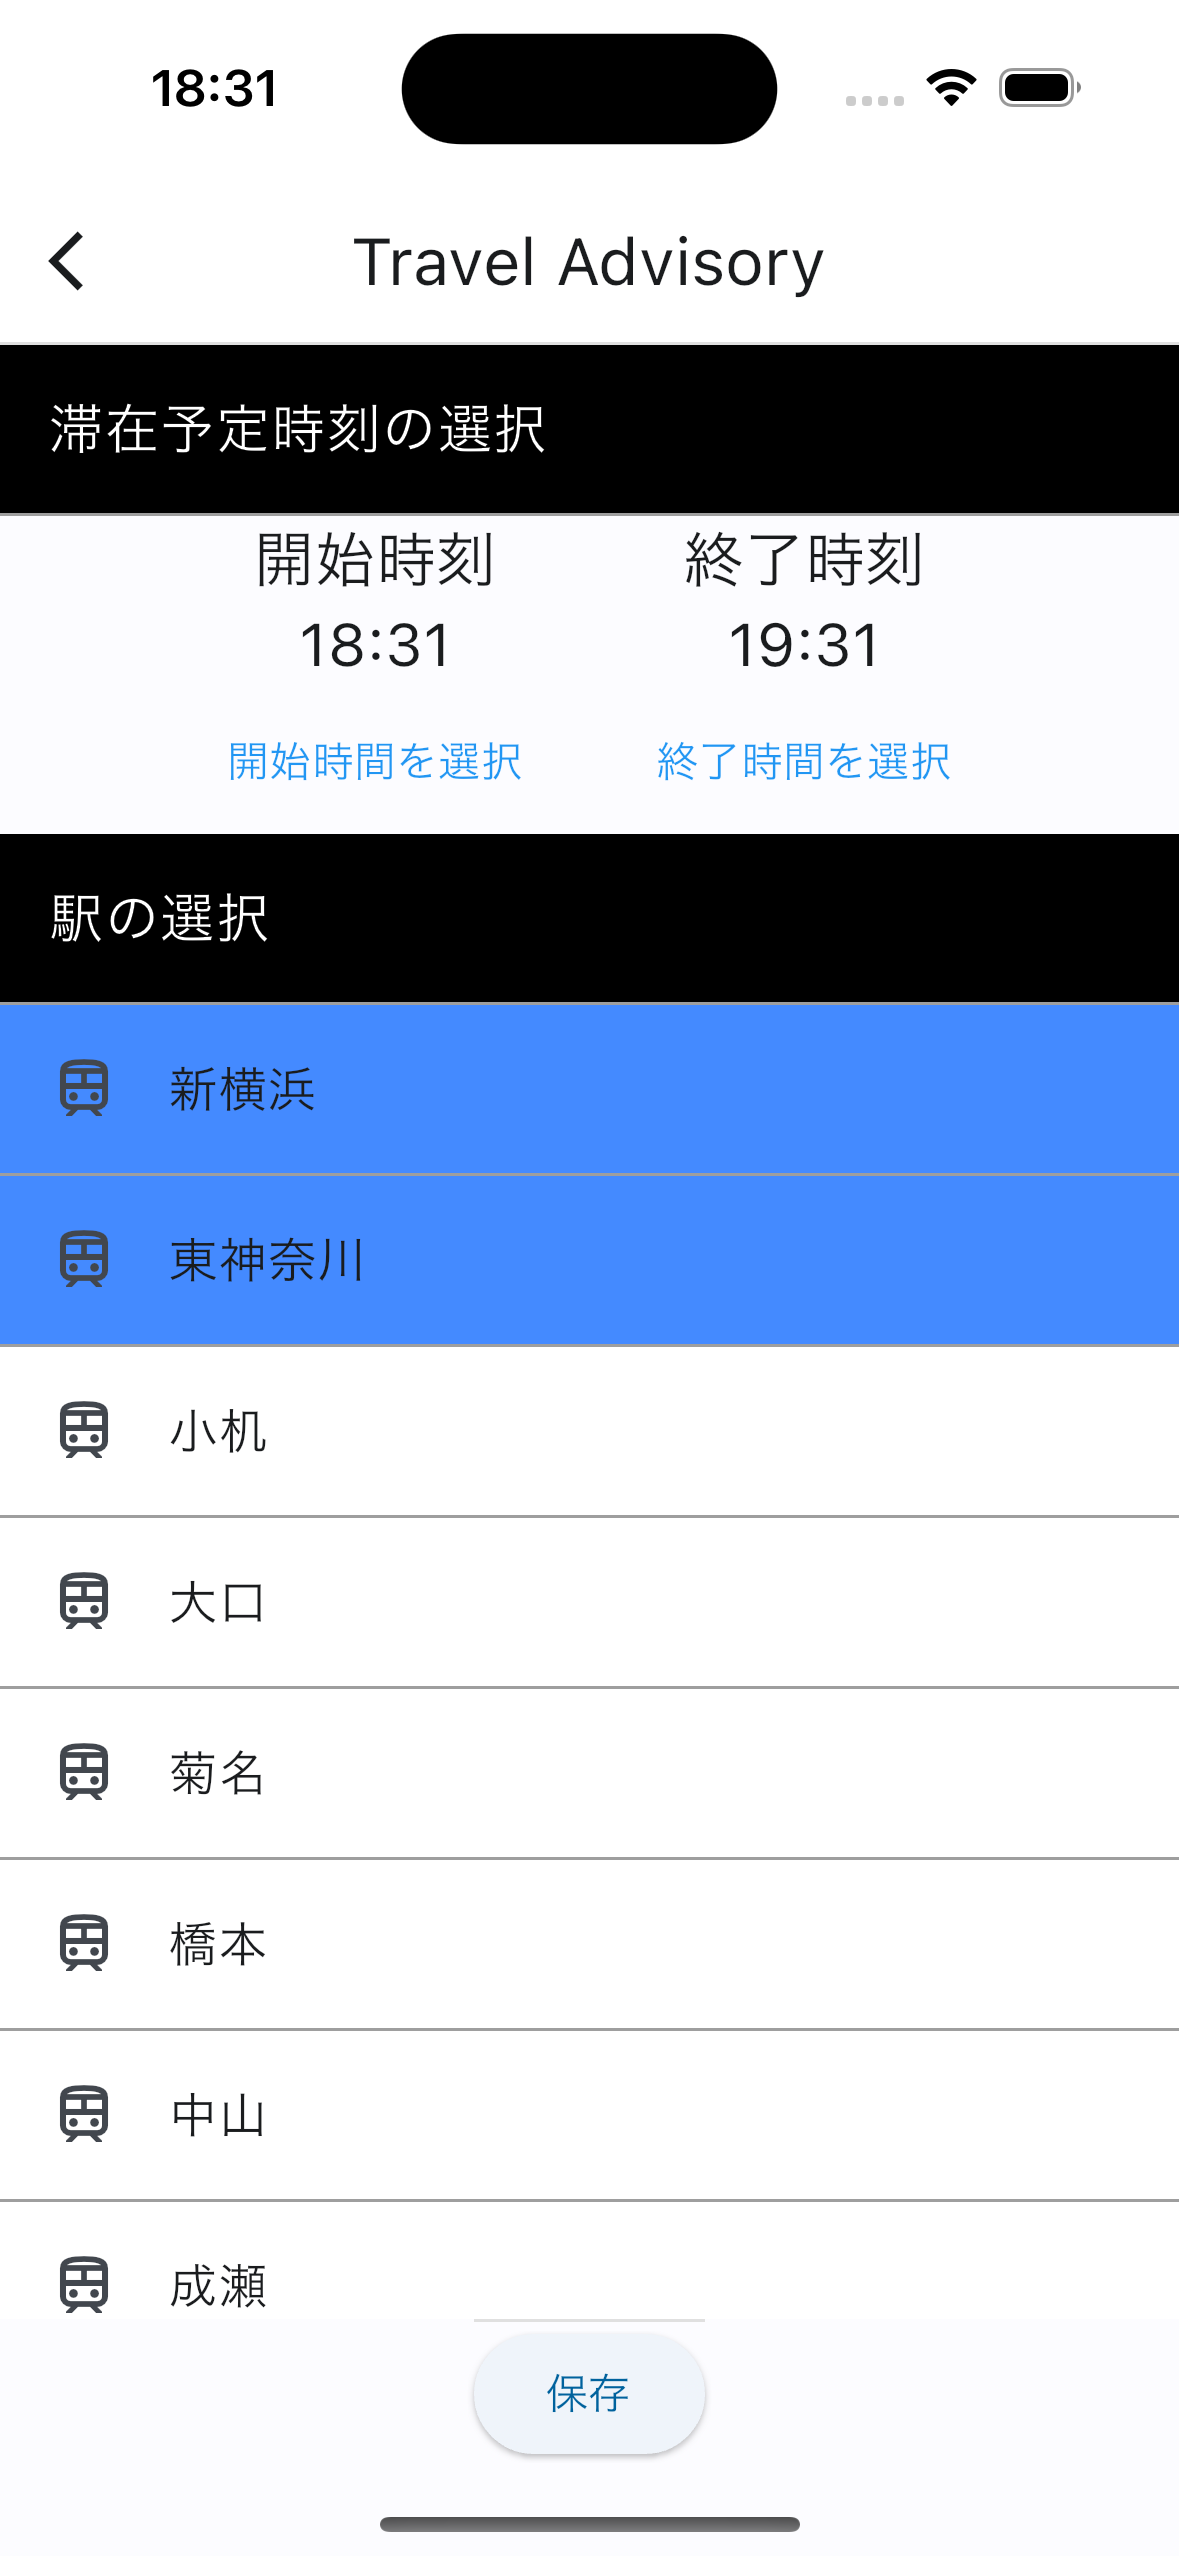
\includegraphics[height=10cm]{./fig/trans_data_save.png}
    %\vspace{-3mm}
    \caption{利用する駅を保存する画面}
    \label{fig:trans_data_save}
    %\vspace{2mm}
  \end{minipage}
\end{figure}

\subsection {通知を受け取る}
通知をタップする.
保存した旅程データがバッチ処理によって災害情報と紐付けられると,push通知が届く.
そしてホーム画面の災害注意予報一覧から注意報が出ている旅程パッケージをタップする.
なお,本アプリにおいては遠隔からの通知を受け取る仕様ではなく,ユーザがアプリを通じて通知を送信する.
本来であれば遠隔から通知を受け取るべきだが,後述する評価実験に関係のない機能であることから本実験では実装を見送った.

\begin{figure}[H]
  \begin{minipage}[b]{0.45\linewidth}
    \centering
    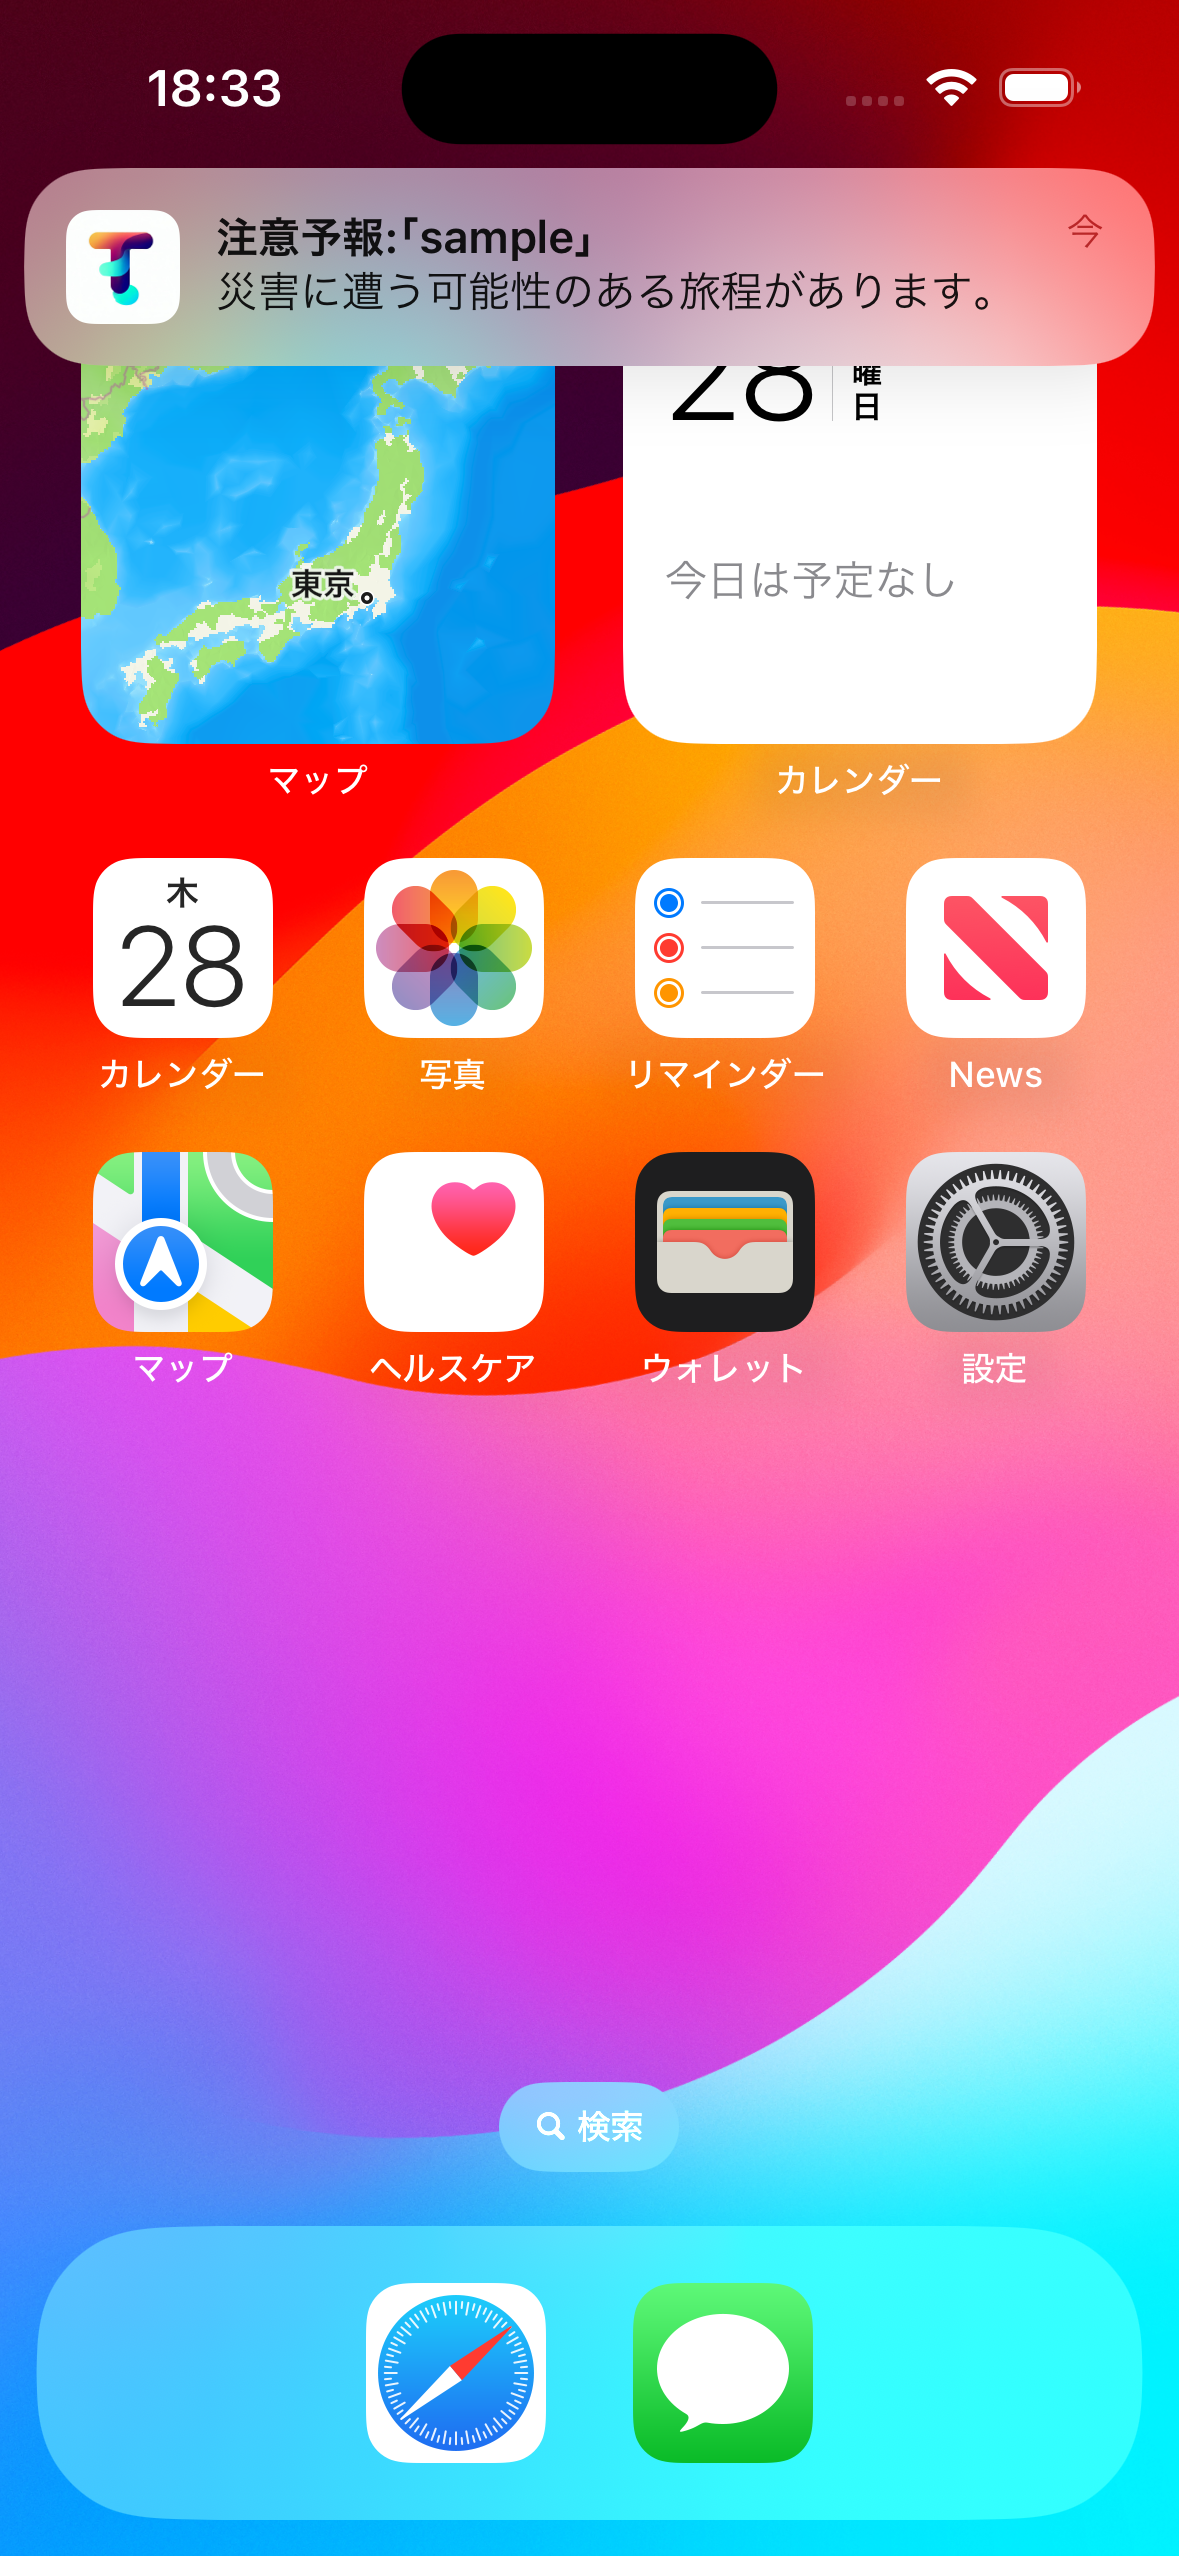
\includegraphics[height=10cm]{./fig/notion.png}
    %\vspace{-3mm}
    \caption{通知の表示}
    \label{fig:notion}
    %\vspace{2mm}
  \end{minipage}
  \begin{minipage}[b]{0.45\linewidth}
    \centering
    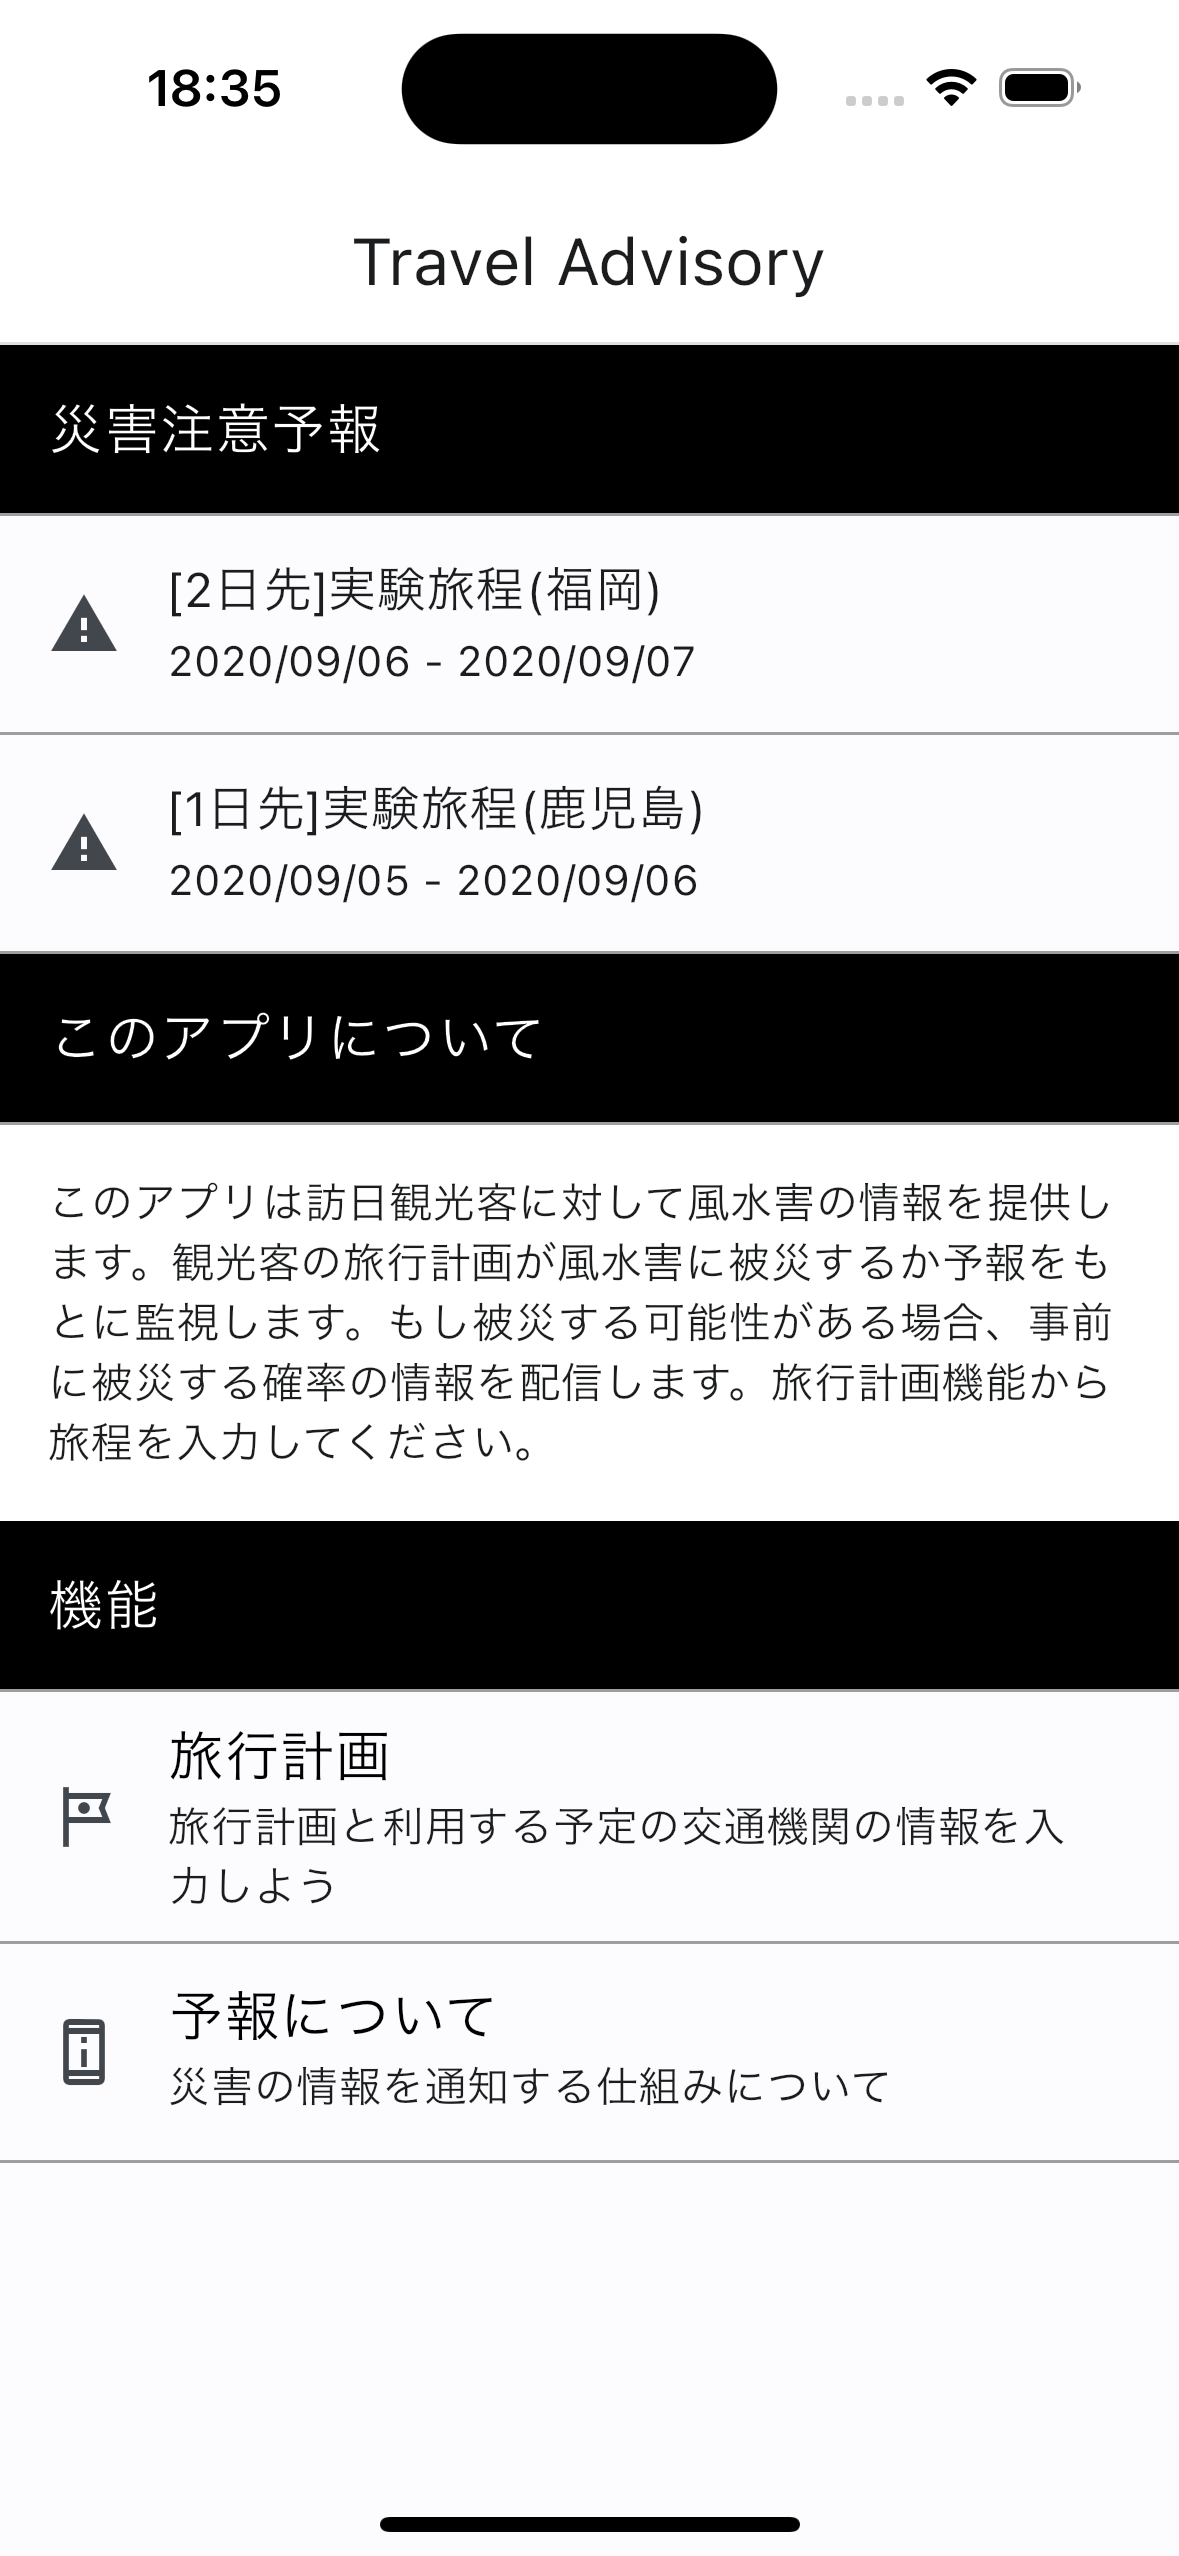
\includegraphics[height=10cm]{./fig/unormal_home_screen.png}
    %\vspace{-3mm}
    \caption{災害注意予報通知時のホーム画面}
    \label{fig:unormal_home_screen}
    %\vspace{2mm}
  \end{minipage}
\end{figure}

\subsection {災害注意予報を確認する}
選択した旅行パッケージの災害注意予報が紐付けられている旅程データの一覧を閲覧する.
一覧から旅程データを選択する.
\begin{figure}[H]
  \centering
  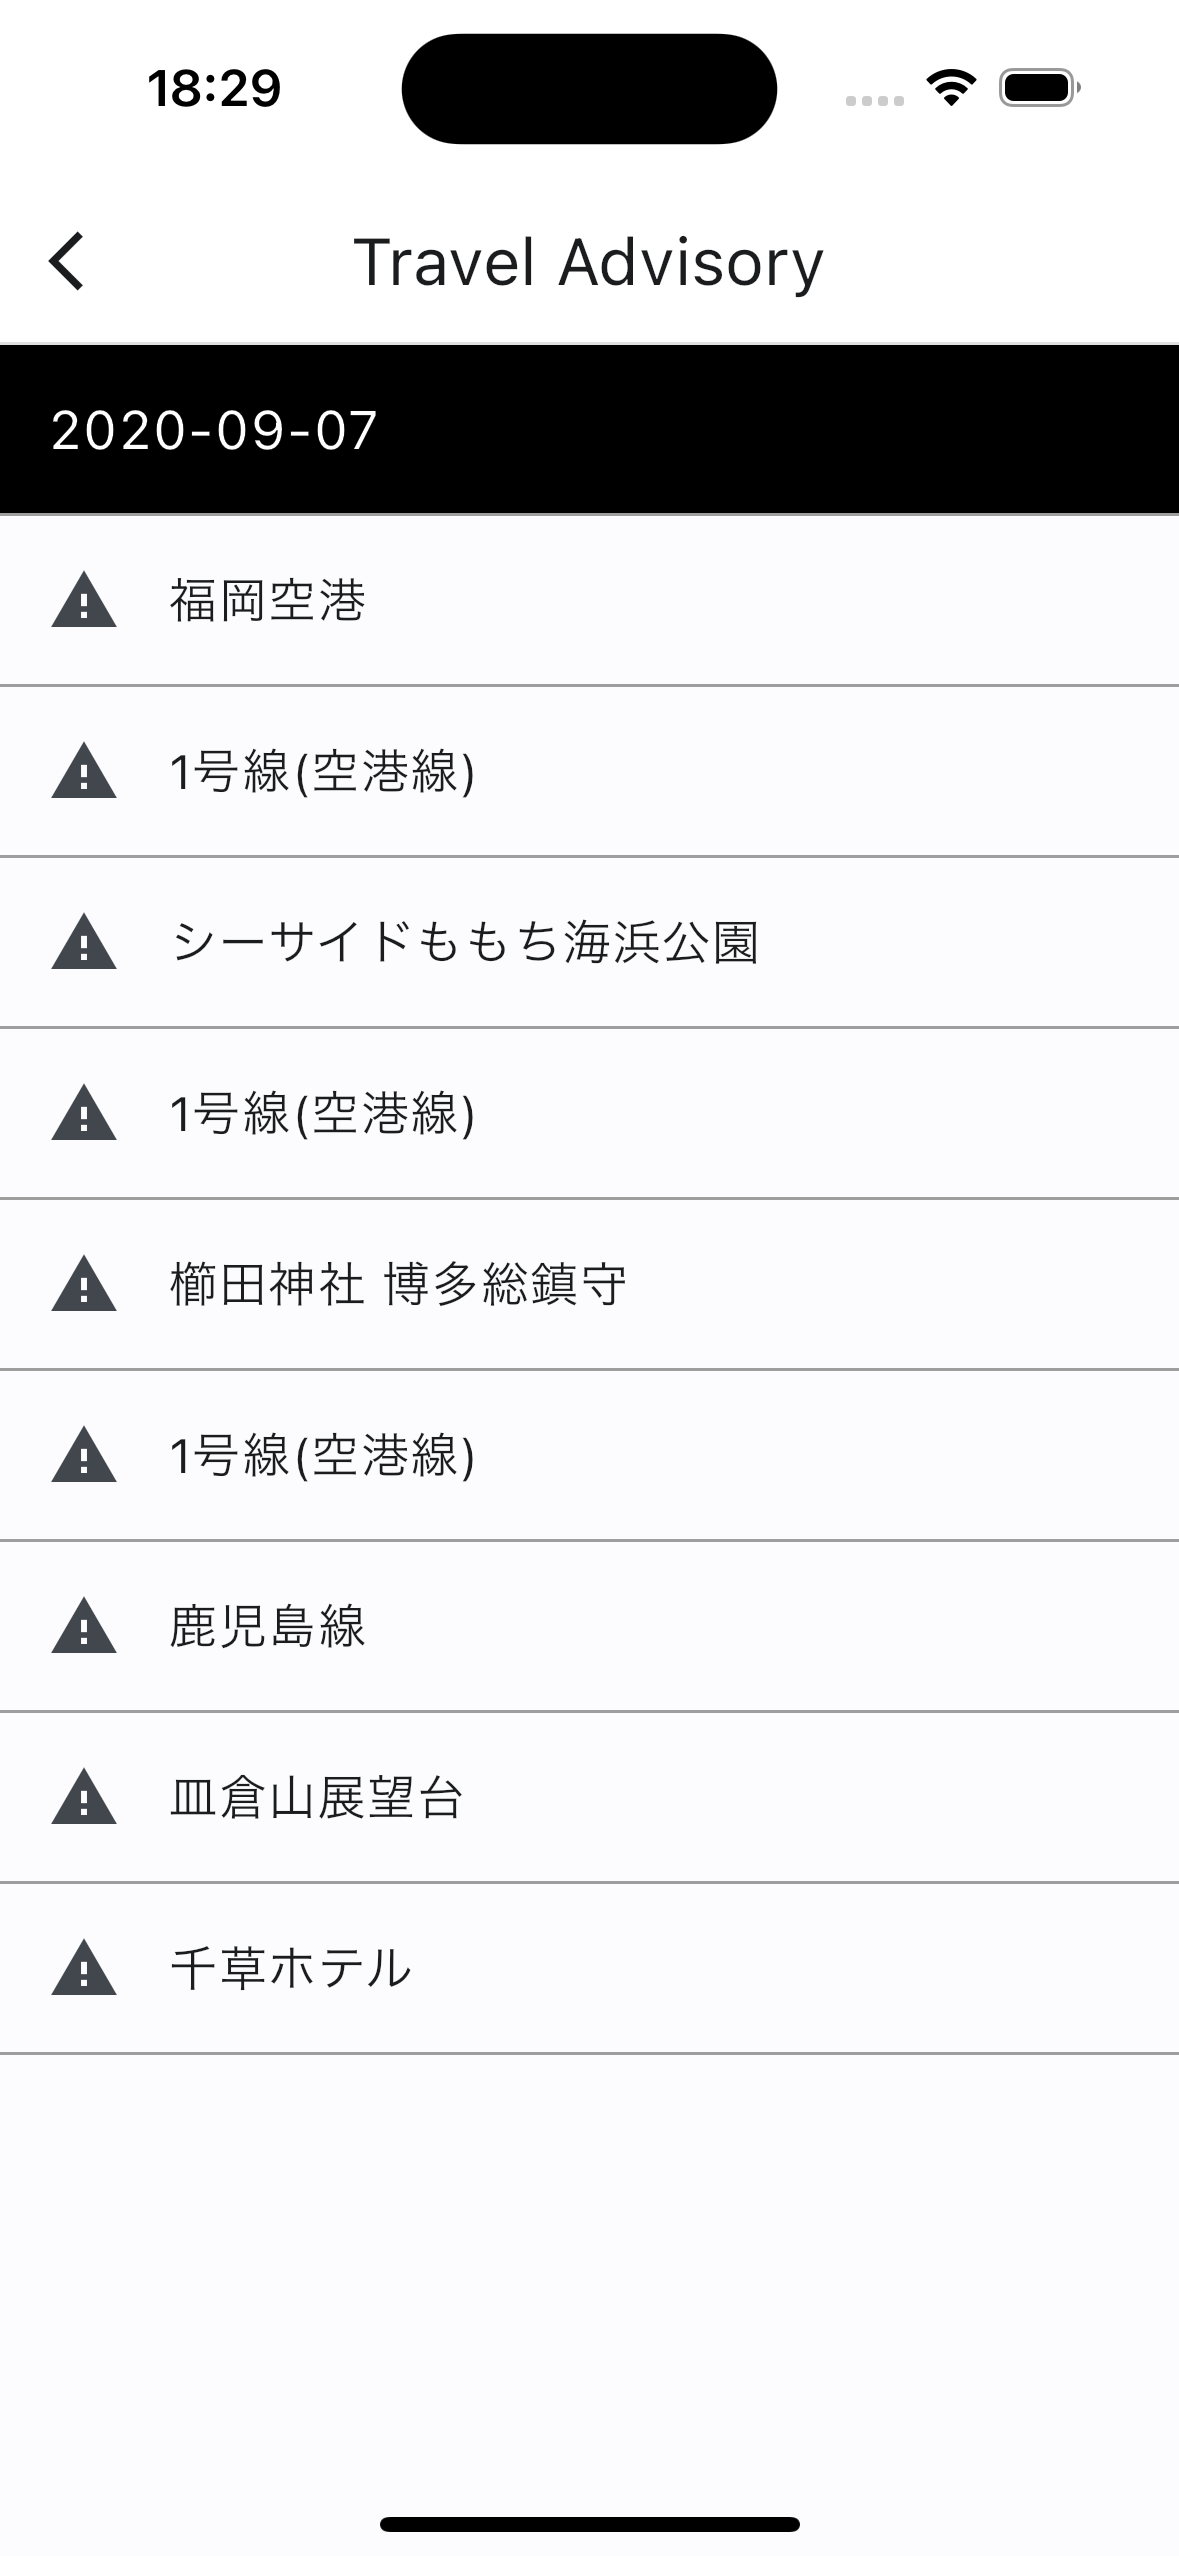
\includegraphics[height=10cm]{./fig/advisory_data_list.png}
  %\vspace{-3mm}
  \caption{災害注意予報が出ている旅程データの一覧}
  \label{fig:advisory_data_list}
  %\vspace{2mm}
\end{figure}

\subsubsection {場所データの災害注意予報}
場所データに対する災害注意予報を閲覧する.
提供される災害の種類は雨と風(風雪)である.災害の種類ごとに災害が起こる確率を提供している.
それぞれの災害のリストをタップすると,ストック情報の画面に遷移する.

\begin{figure}[H]
  \centering
  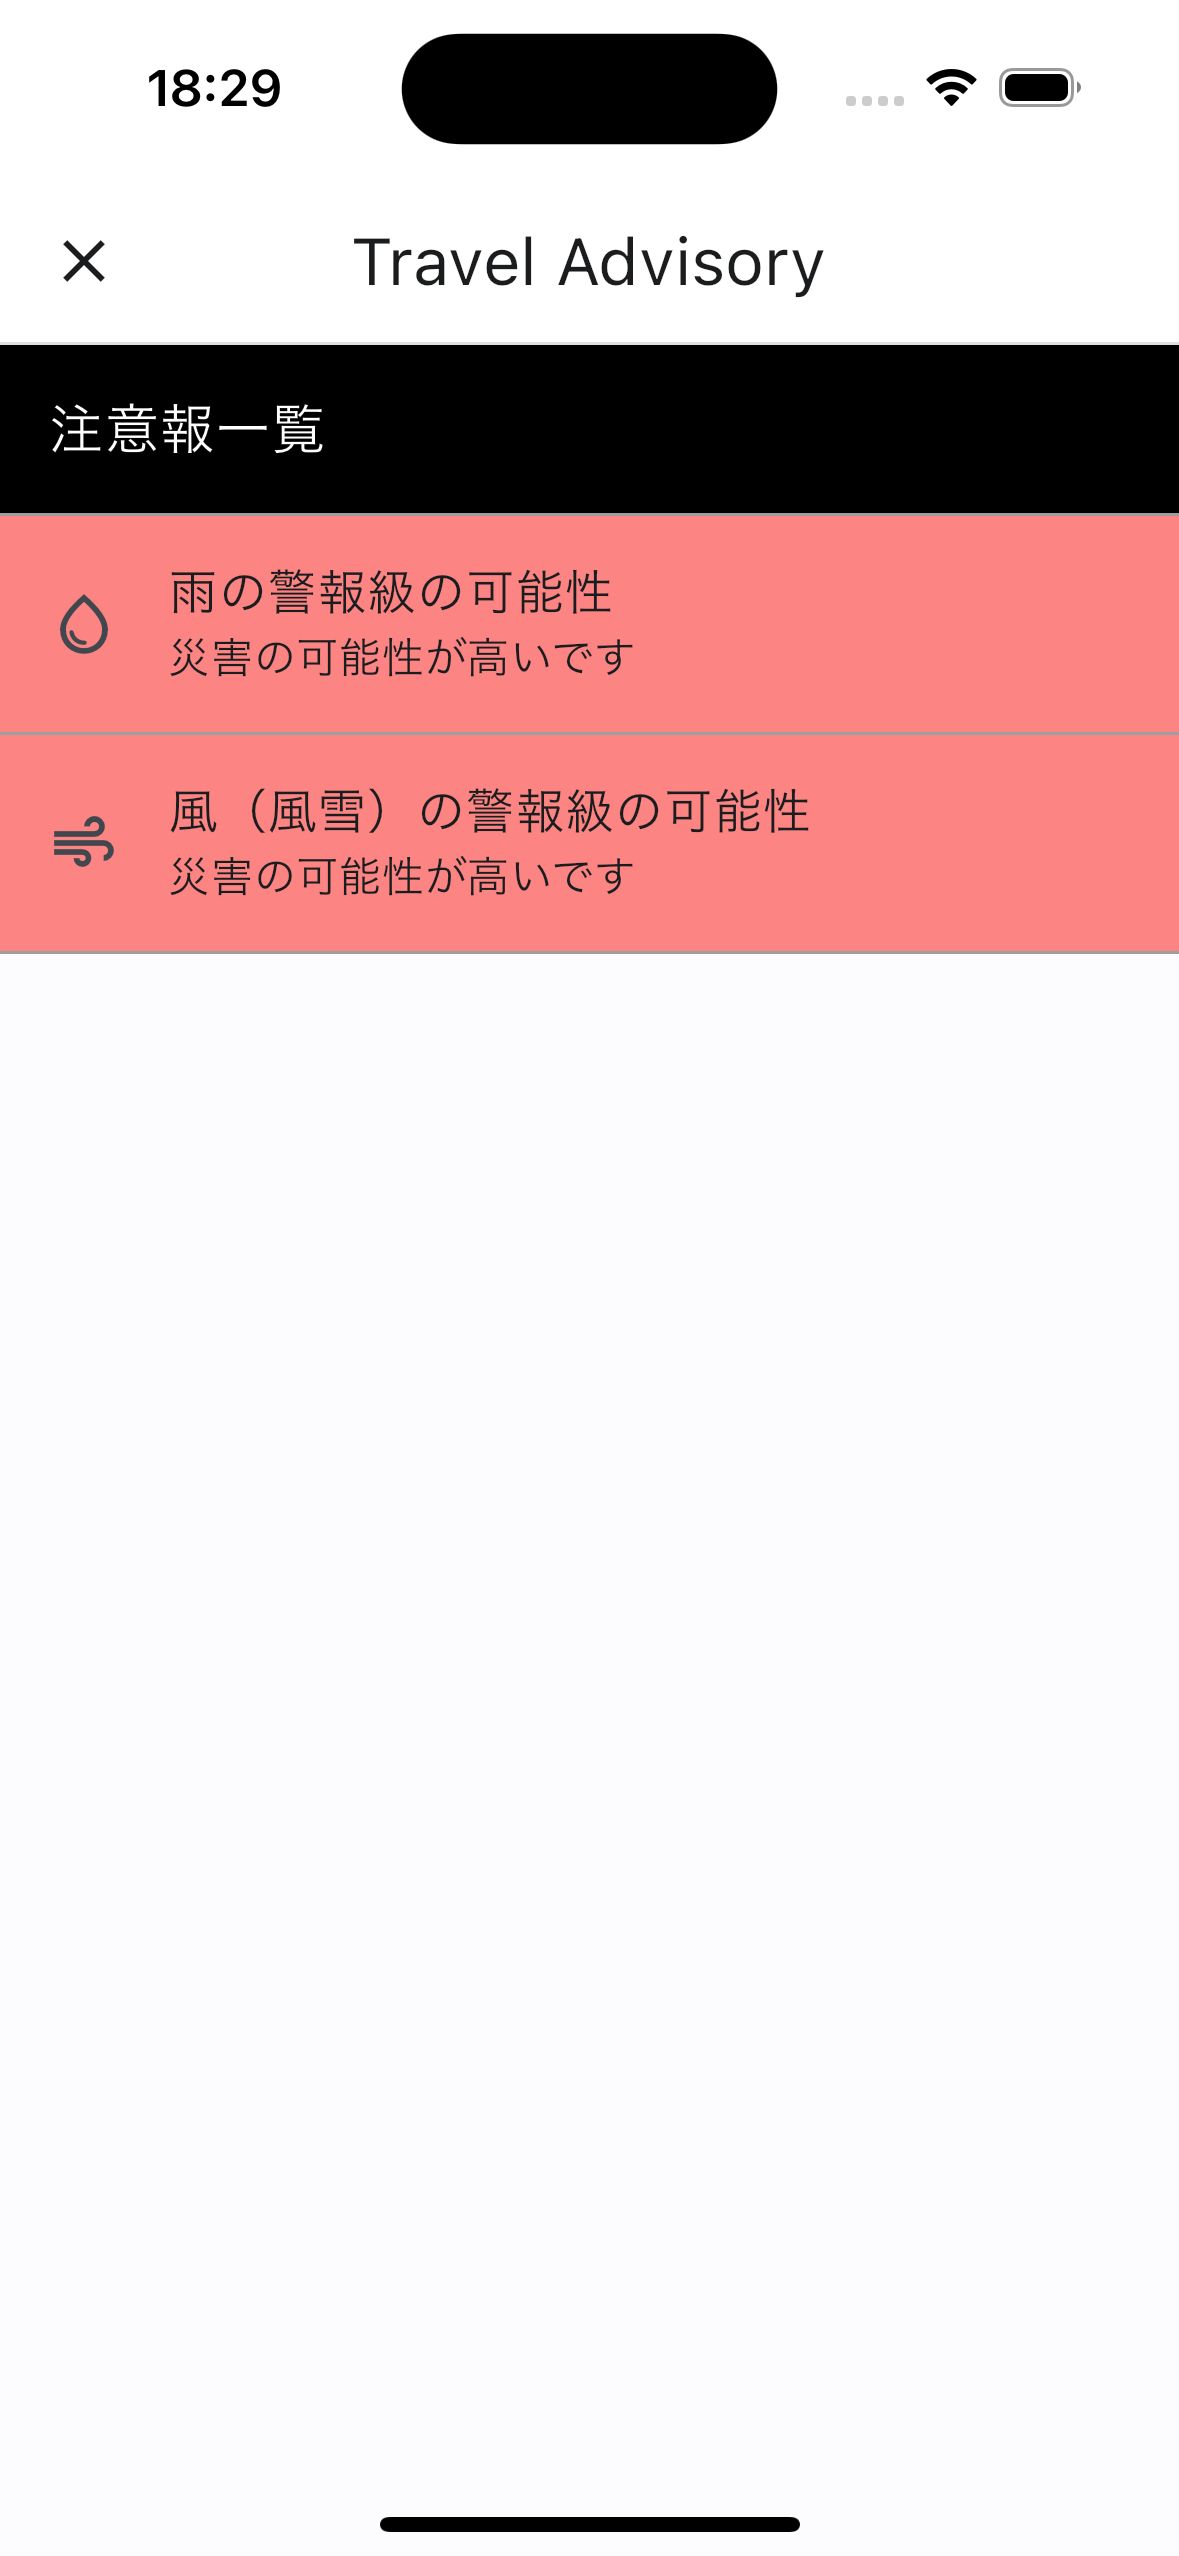
\includegraphics[height=10cm]{./fig/spot_advisory.png}
  %\vspace{-3mm}
  \caption{場所データの災害注意予報画面}
  \label{fig:spot_advisory}
  %\vspace{2mm}
\end{figure}

\subsubsection {交通データの災害注意予報}
交通データに対する災害注意予報を閲覧する.
交通データにおいては,場所データと同じように駅データごとに災害注意予報が提供される.
各駅に対して災害の発生する可能性を運休する可能性として情報を提供している.
さらに,ページ下部には災害時に起こる交通機関の運休の現象や計画運休の現象についての説明がある.

\begin{figure}[H]
  \begin{minipage}[b]{0.45\linewidth}
    \centering
    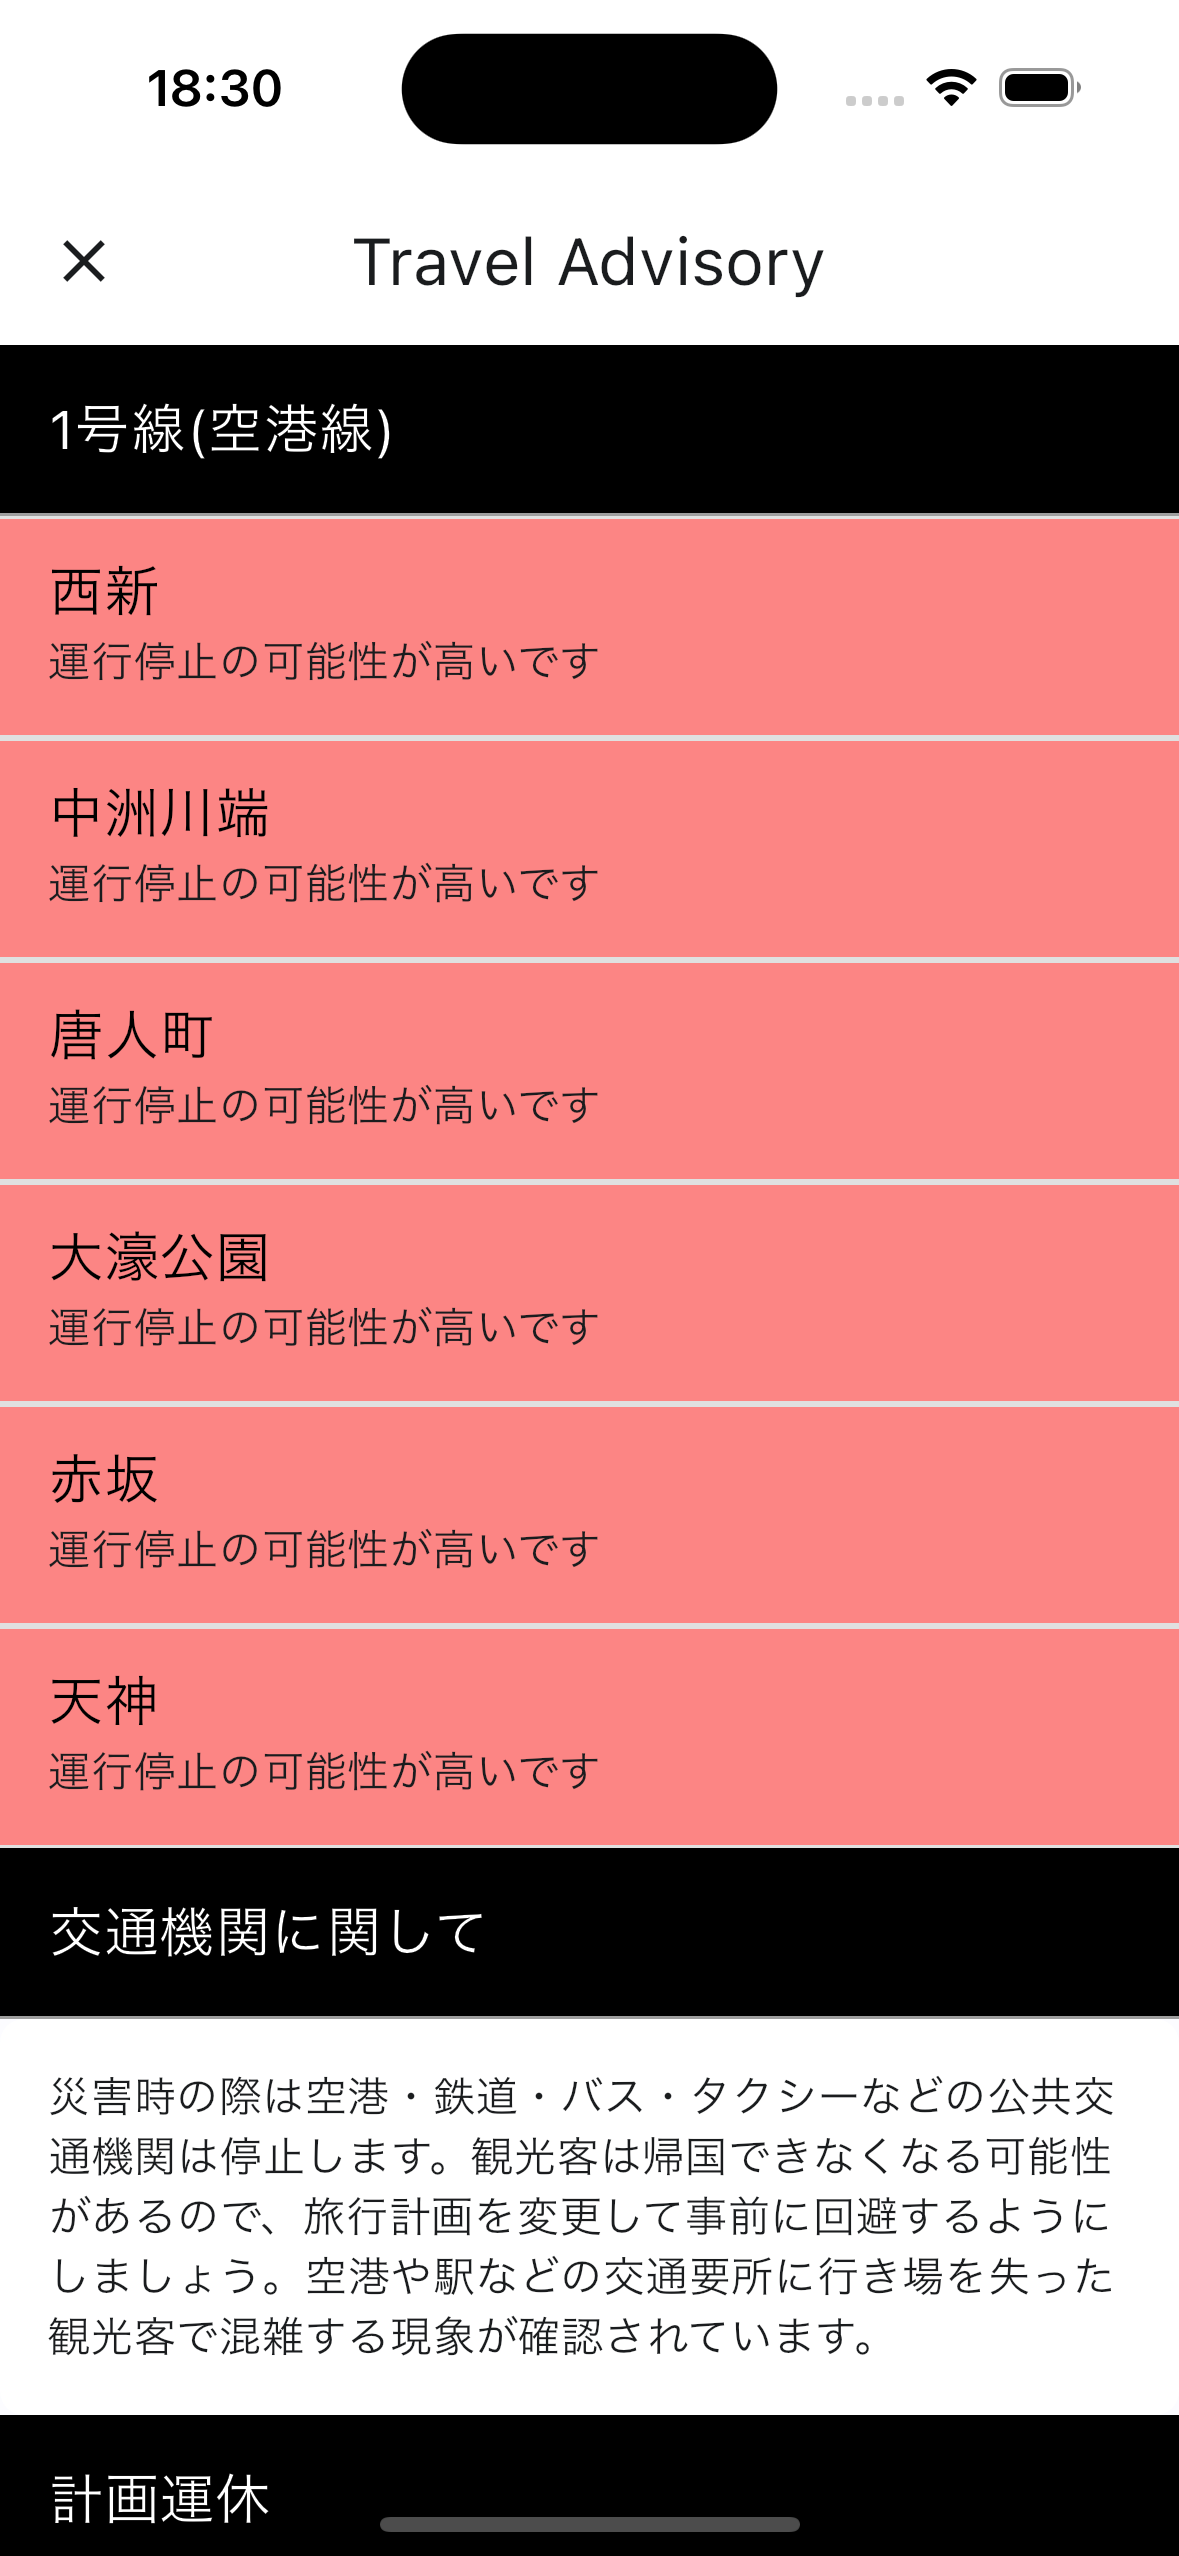
\includegraphics[height=10cm]{./fig/trans_advisory_1.png}
    %\vspace{-3mm}
    \caption{交通データの災害注意予報画面1}
    \label{fig:trans_advisory_1}
    %\vspace{2mm}
  \end{minipage}
  \begin{minipage}[b]{0.45\linewidth}
    \centering
    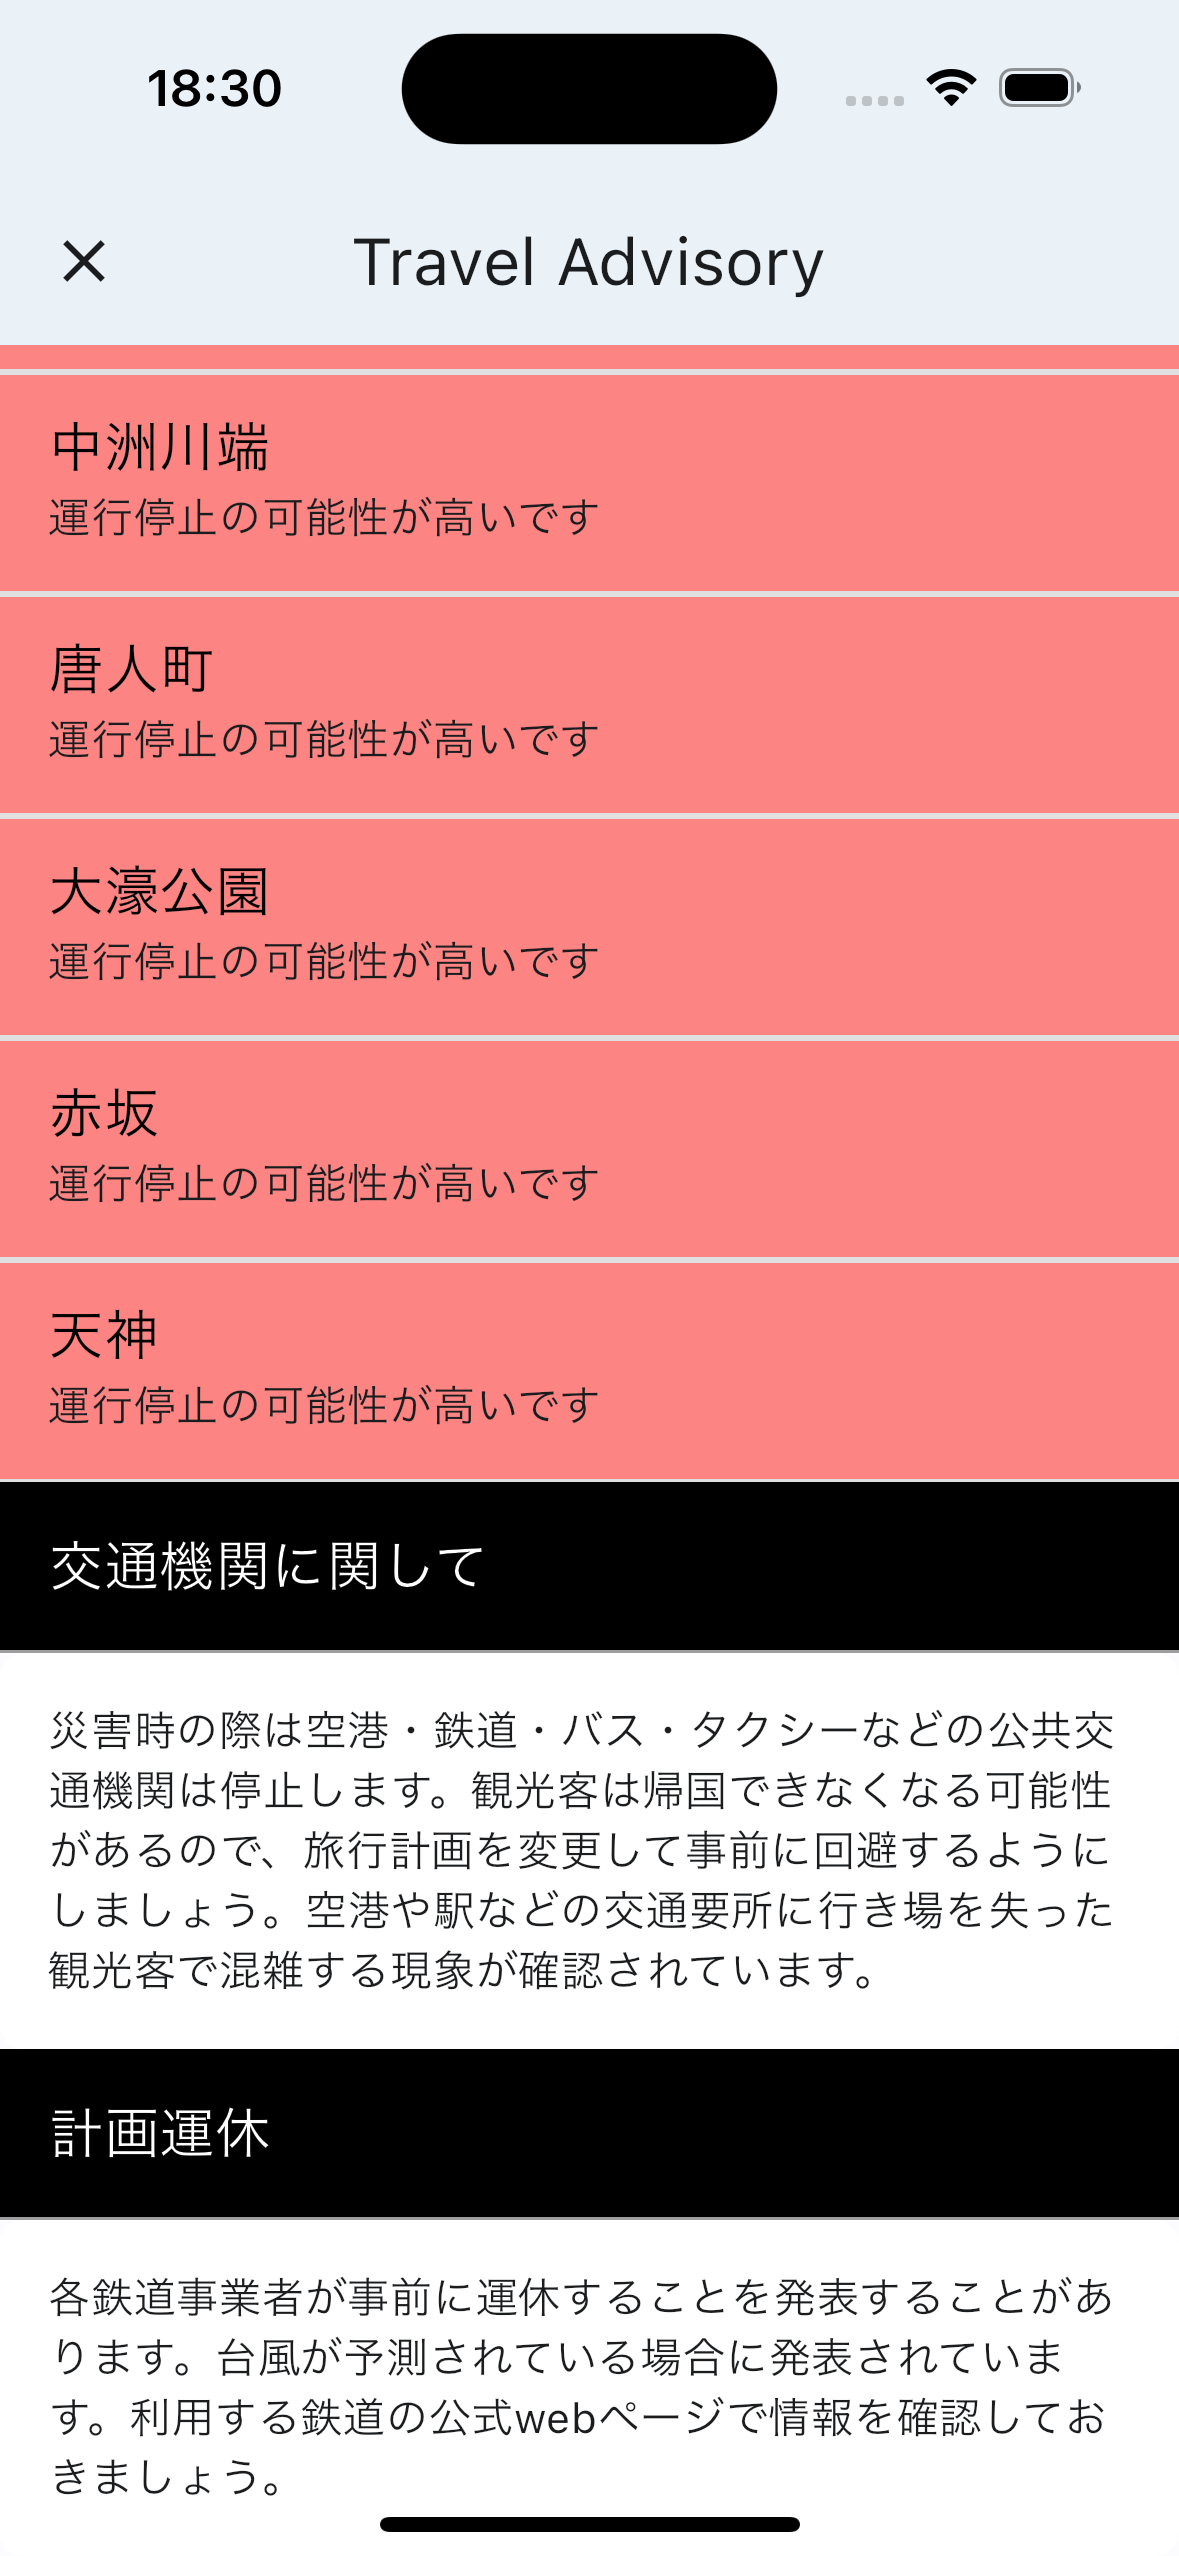
\includegraphics[height=10cm]{./fig/trans_advisory_2.png}
    %\vspace{-3mm}
    \caption{交通データの災害注意予報画面2}
    \label{fig:trans_advisory_2}
    %\vspace{2mm}
  \end{minipage}
\end{figure}

\subsection {ストック情報を確認する}
災害のストック情報を閲覧する.
ストック情報は雨と風(風雪)の2種類の災害の情報である.

\subsubsection {雨の災害の情報}
日本における雨に関する災害についての説明が記載されている.
雨に関する災害とは大雨そのものの現象以外に洪水と土砂災害のことである.
各災害についての説明とそれに対する対策喚起の情報が載っている.

\begin{figure}[H]
  \begin{minipage}[b]{0.45\linewidth}
    \centering
    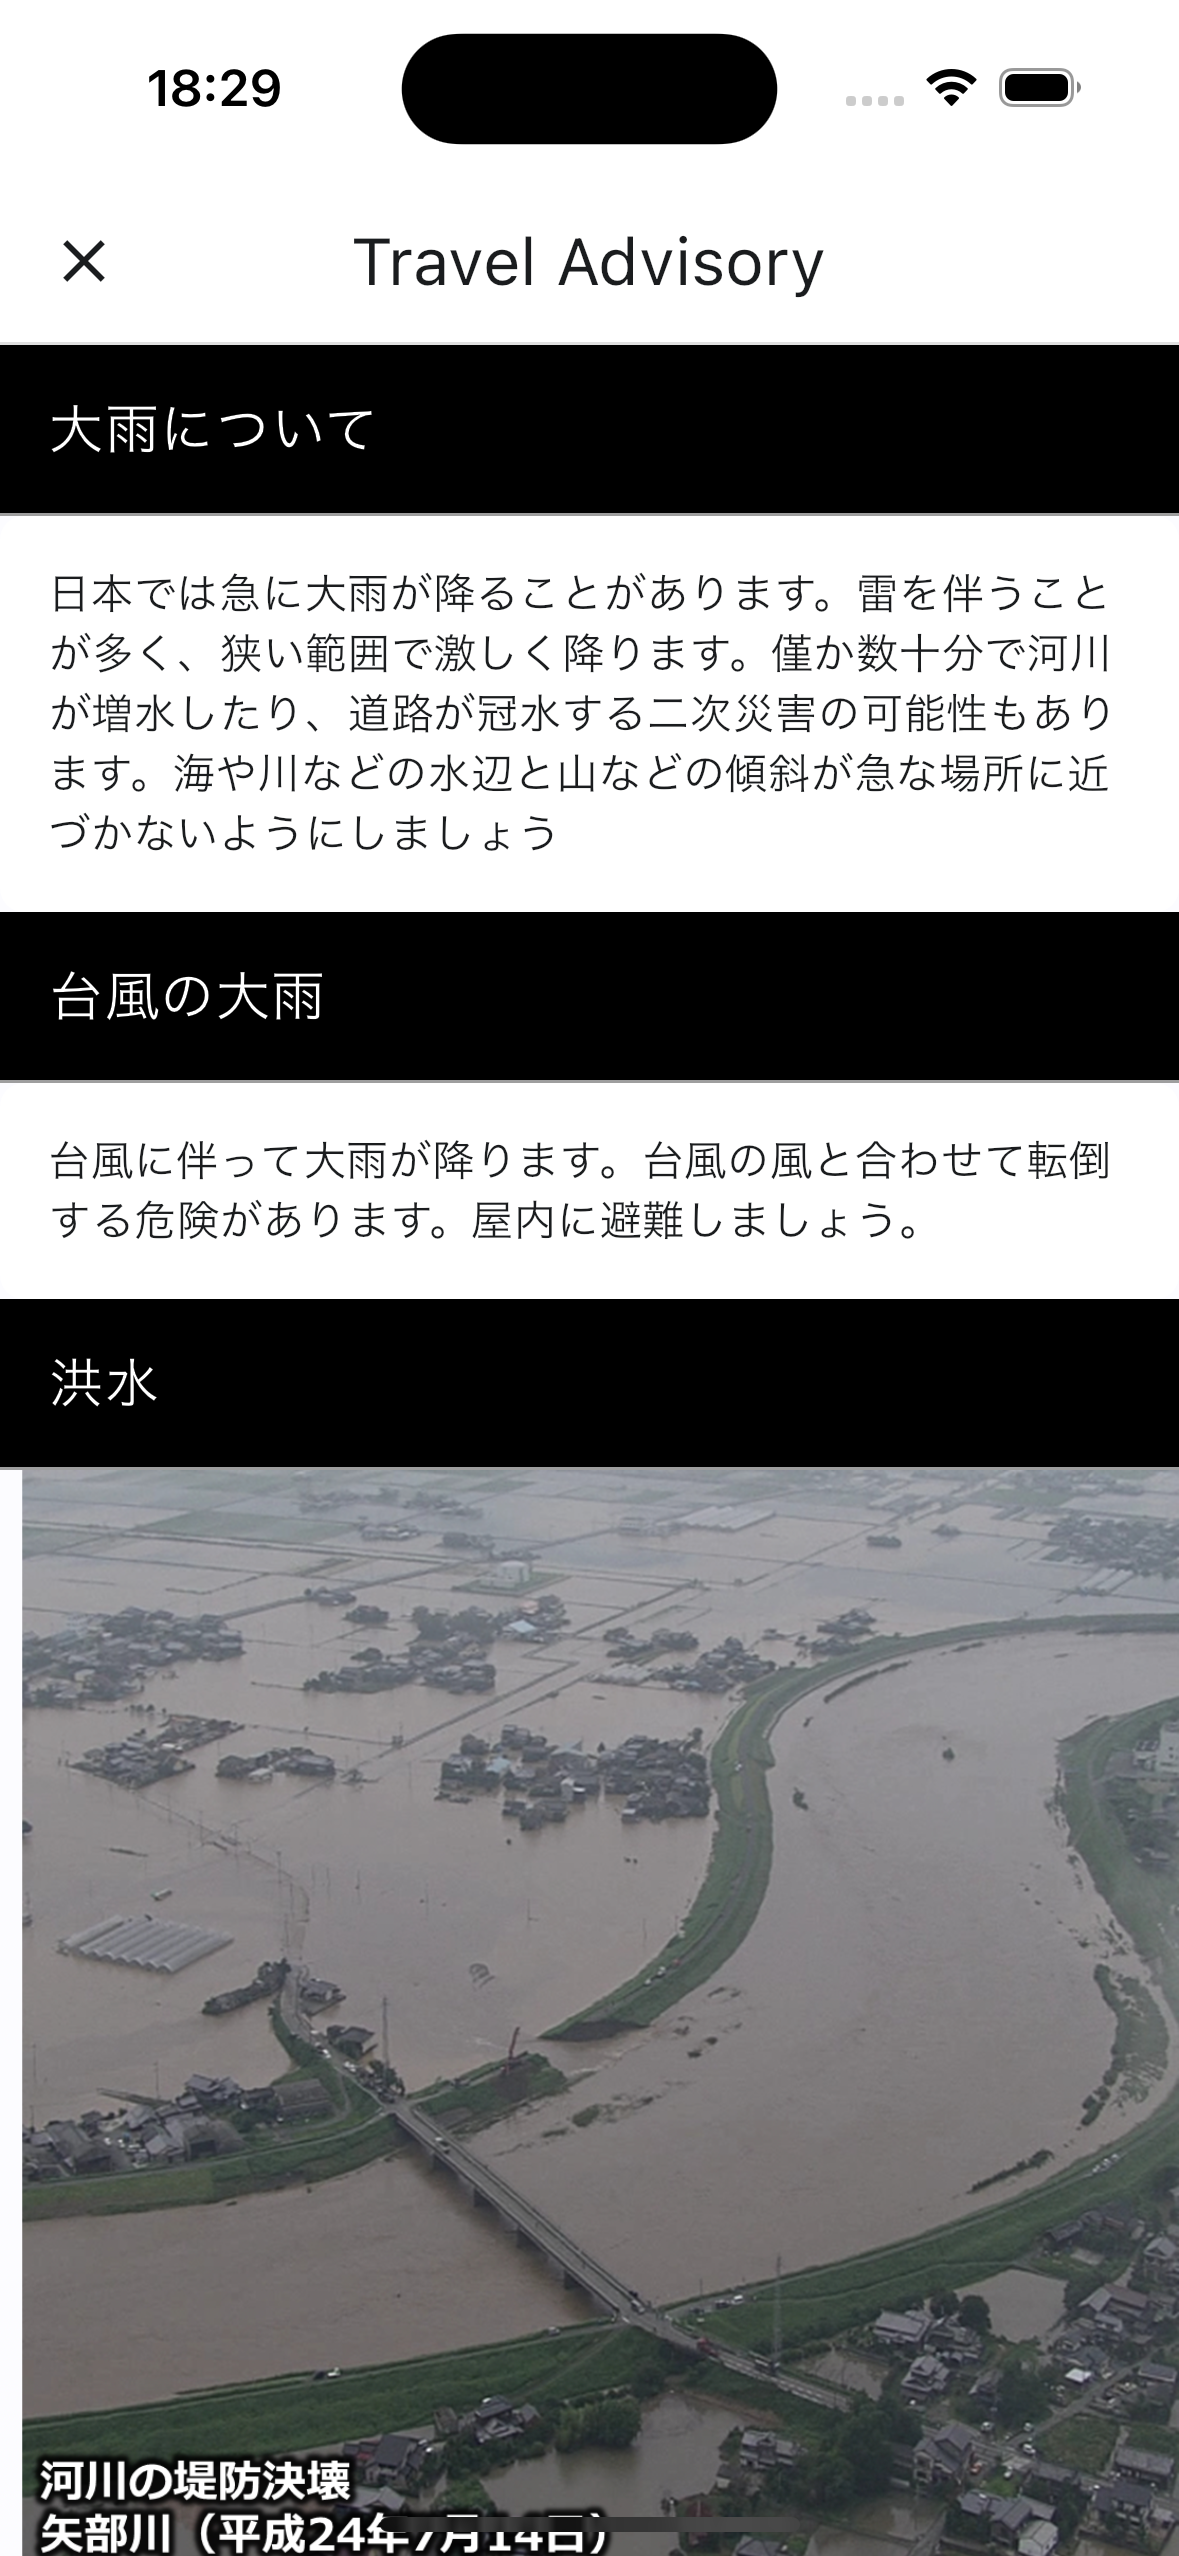
\includegraphics[height=10cm]{./fig/rain_stock_1.png}
    %\vspace{-3mm}
    \caption{雨のストック情報提供画面1}
    \label{fig:rain_stock_1}
    %\vspace{2mm}
  \end{minipage}
  \begin{minipage}[b]{0.45\linewidth}
    \centering
    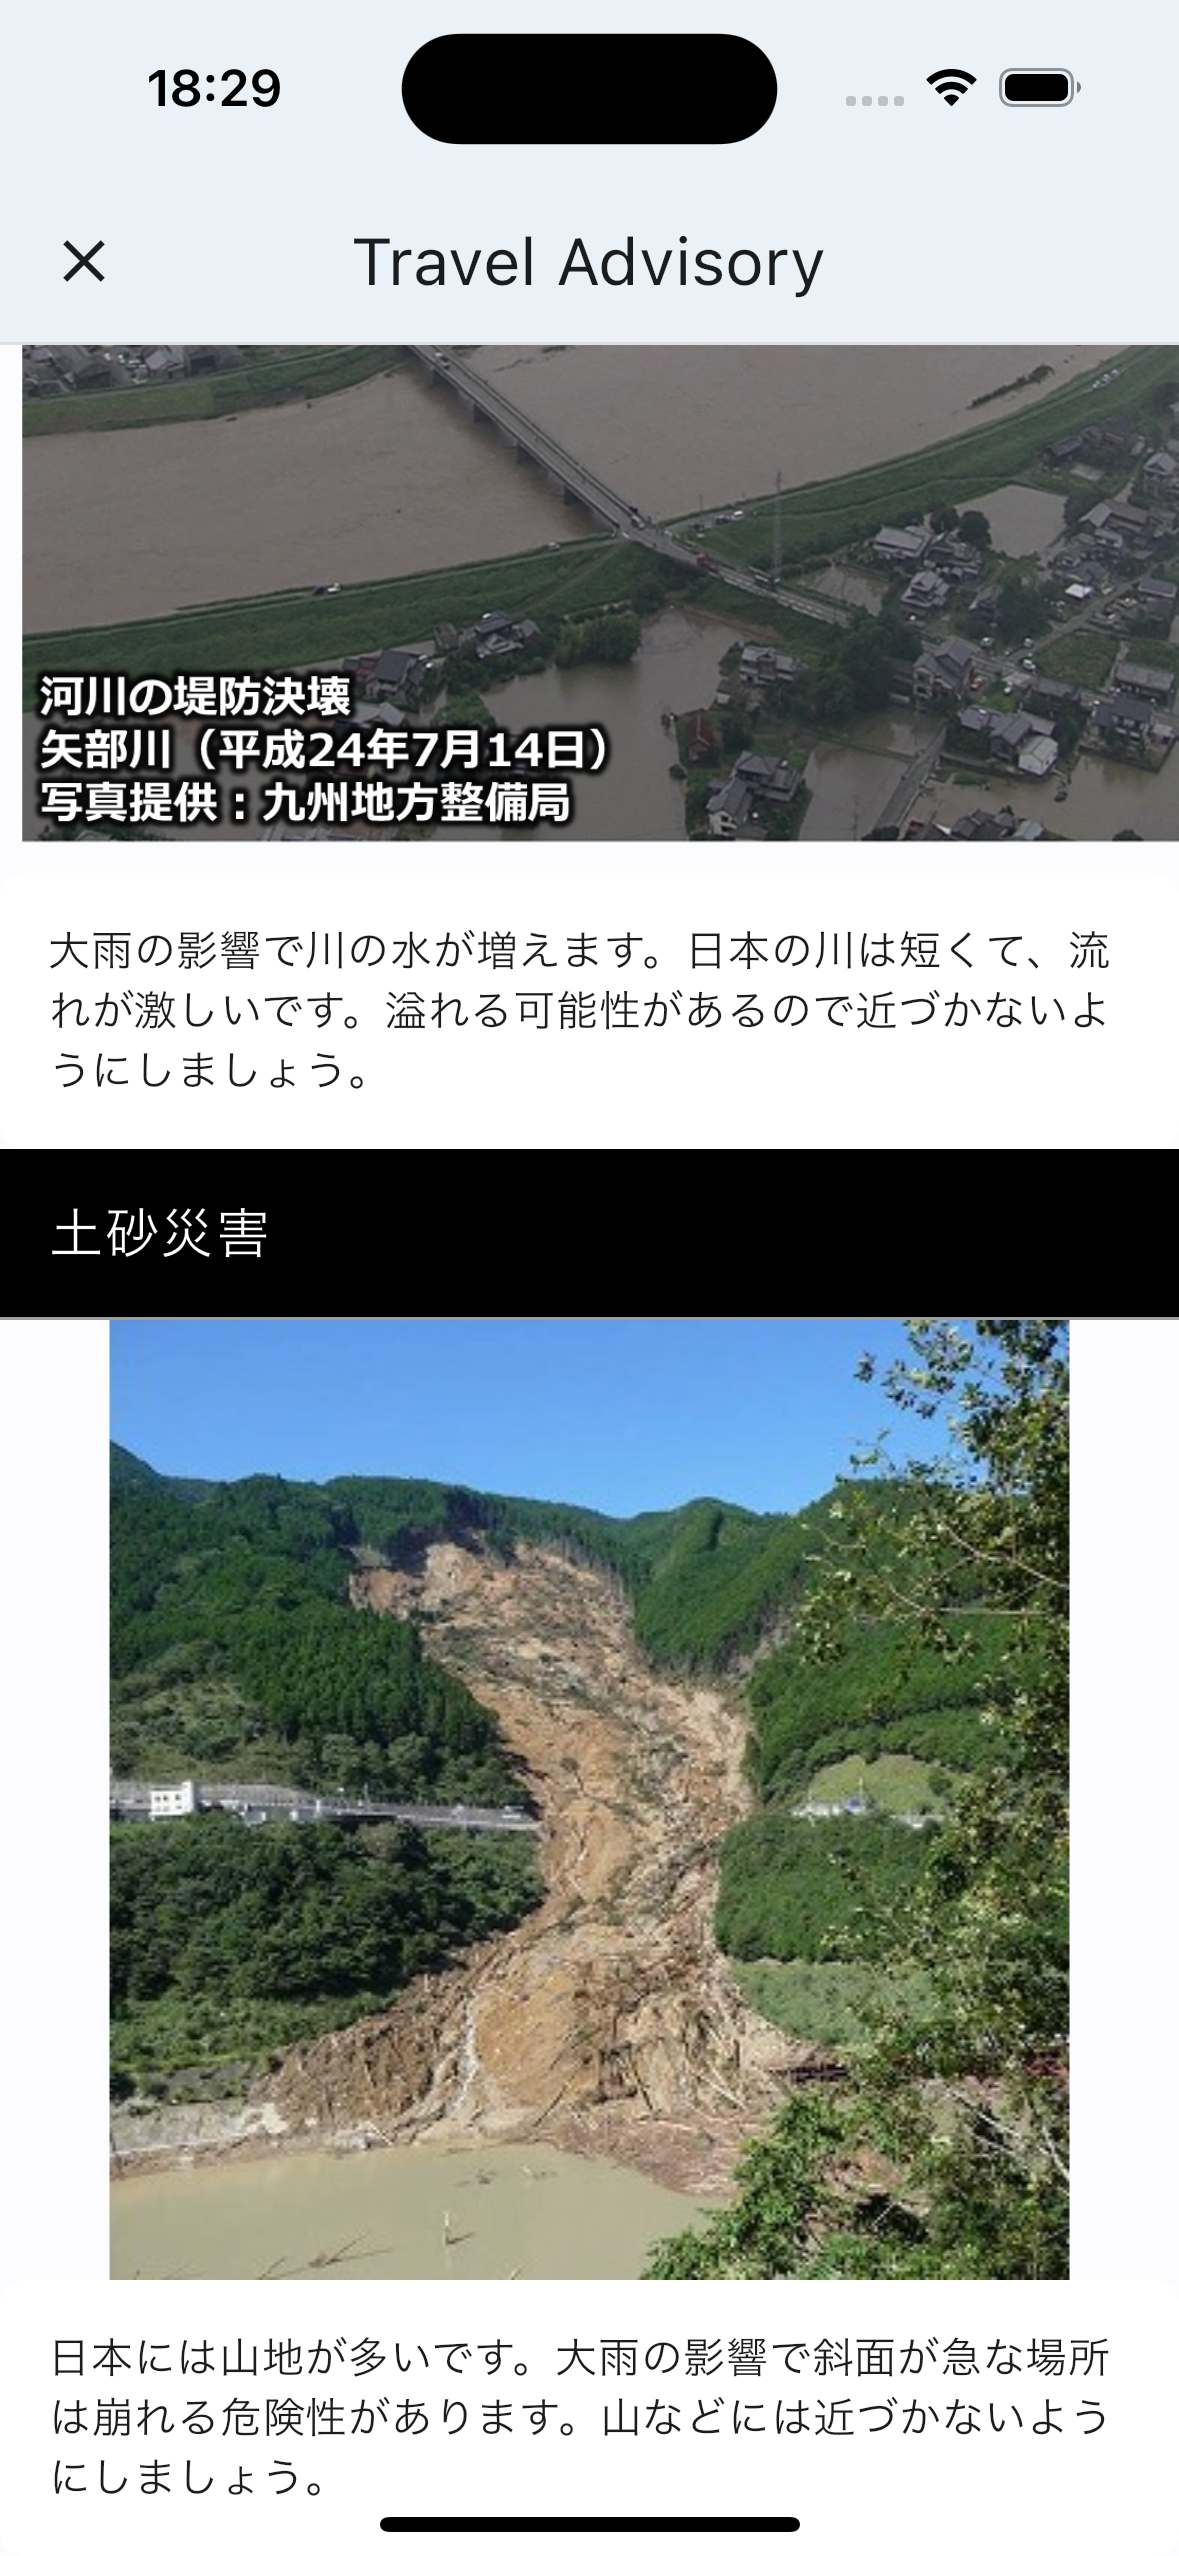
\includegraphics[height=10cm]{./fig/rain_stock_2.png}
    %\vspace{-3mm}
    \caption{雨のストック情報提供画面2}
    \label{fig:rain_stock_2}
    %\vspace{2mm}
  \end{minipage}
\end{figure}

\subsubsection {風の災害の情報}
日本における風に関する災害についての説明が記載されている.
具体的には台風と高潮,暴風についてである.
各災害についての説明とそれに対する対策喚起の情報が載っている.

\begin{figure}[H]
  \begin{minipage}[b]{0.45\linewidth}
    \centering
    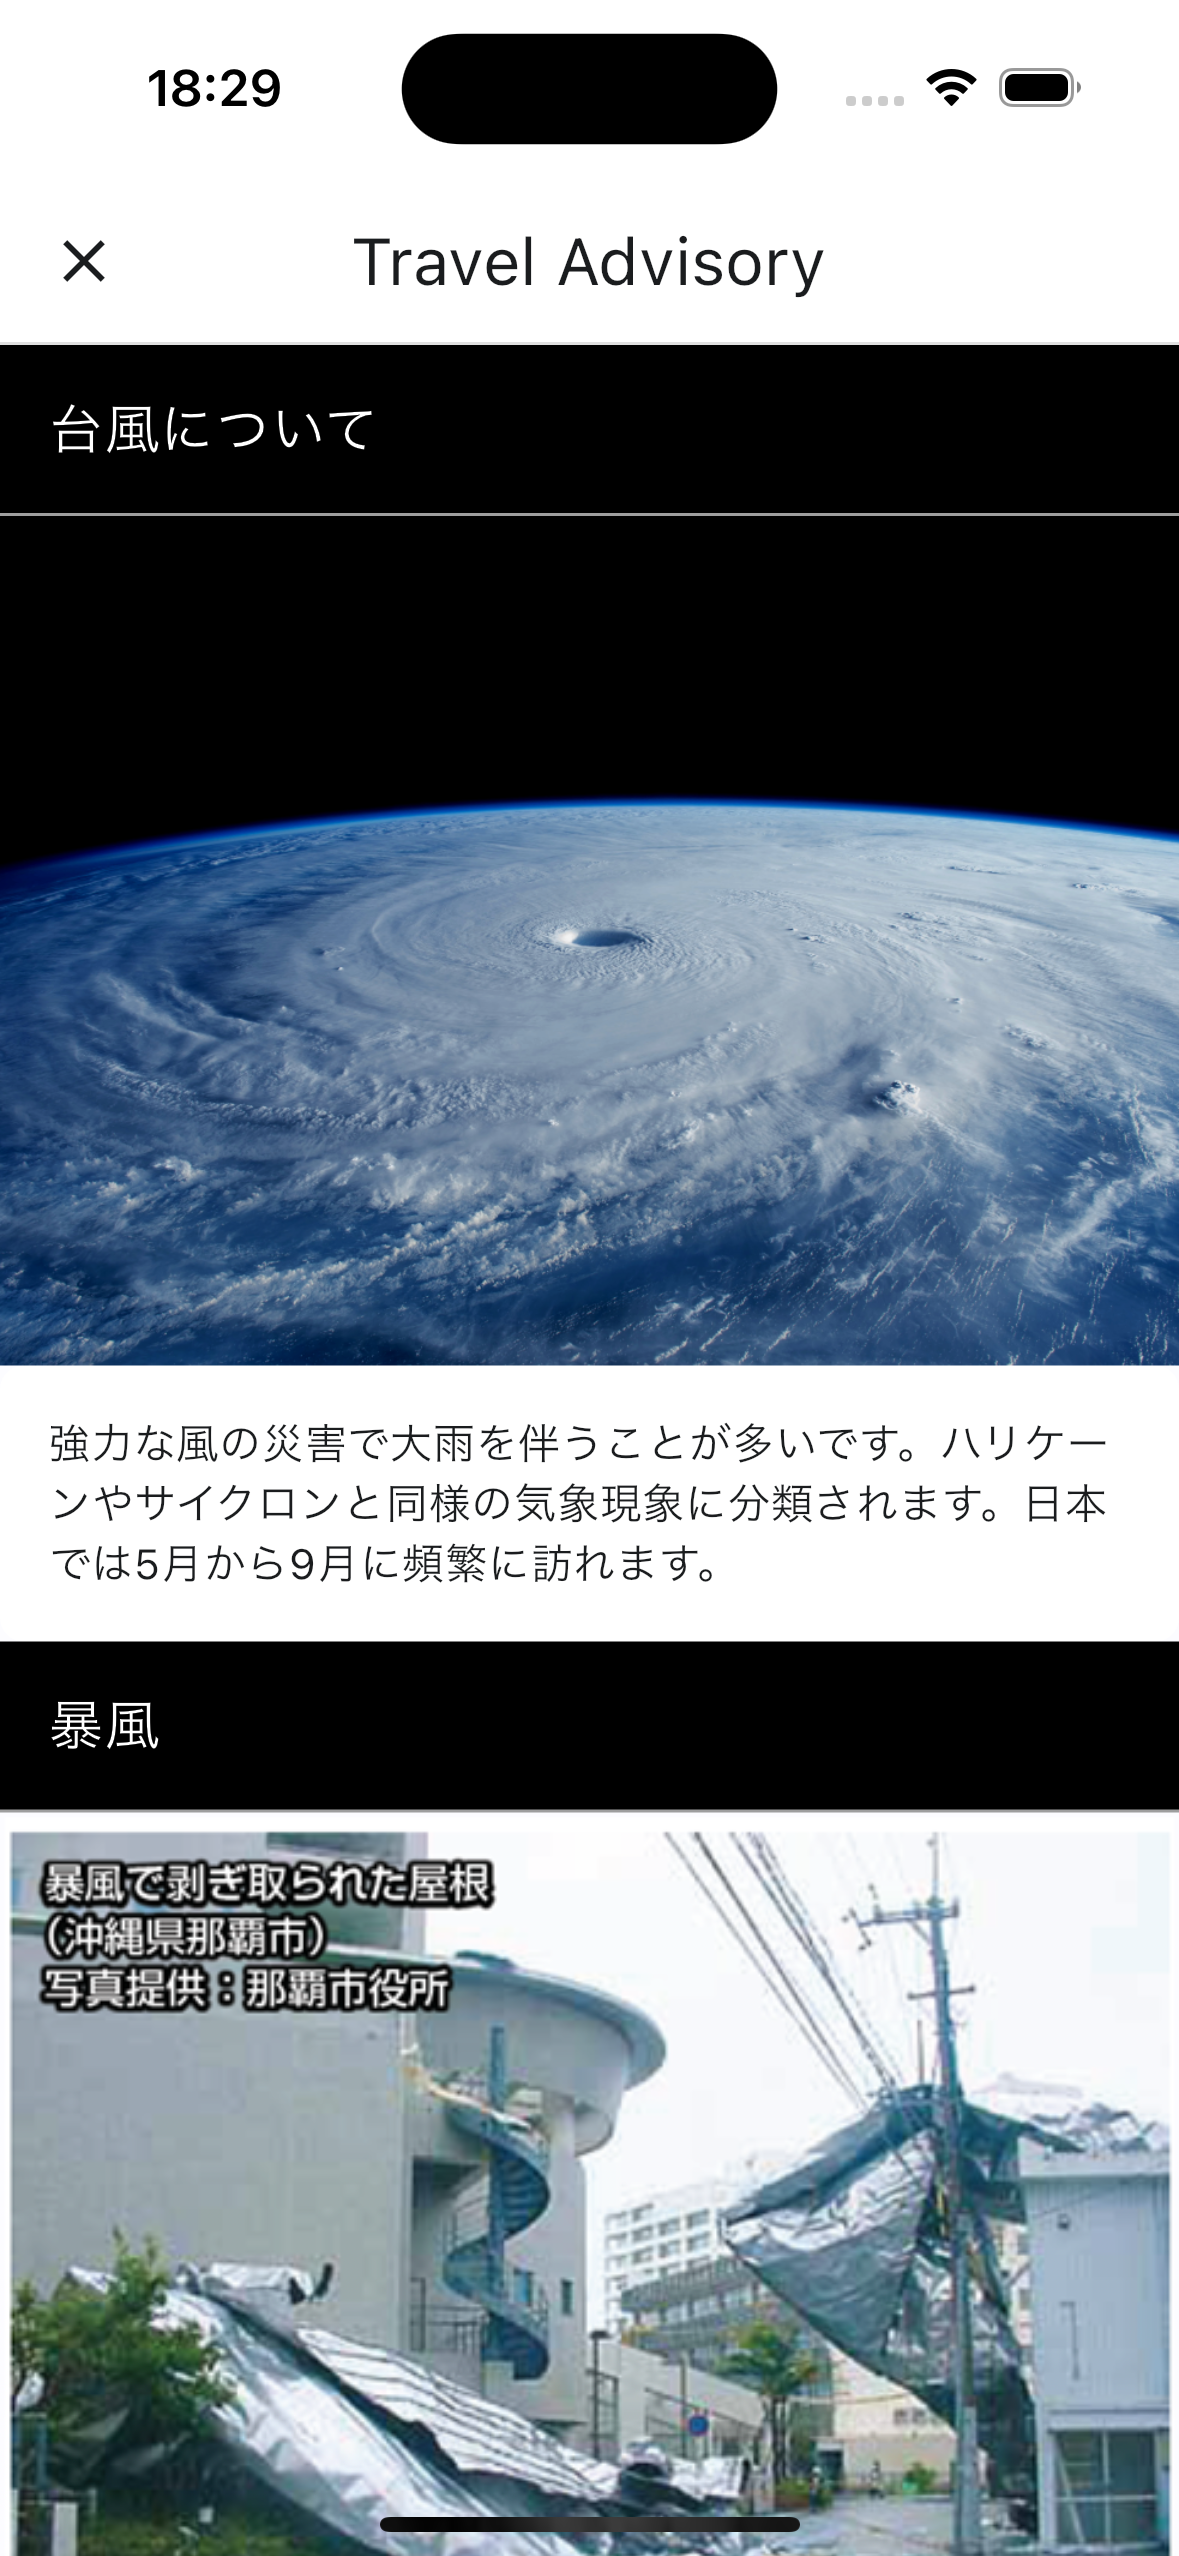
\includegraphics[height=10cm]{./fig/wind_stock_1.png}
    %\vspace{-3mm}
    \caption{風のストック情報提供画面1}
    \label{fig:rain_stock_1}
    %\vspace{2mm}
  \end{minipage}
  \begin{minipage}[b]{0.45\linewidth}
    \centering
    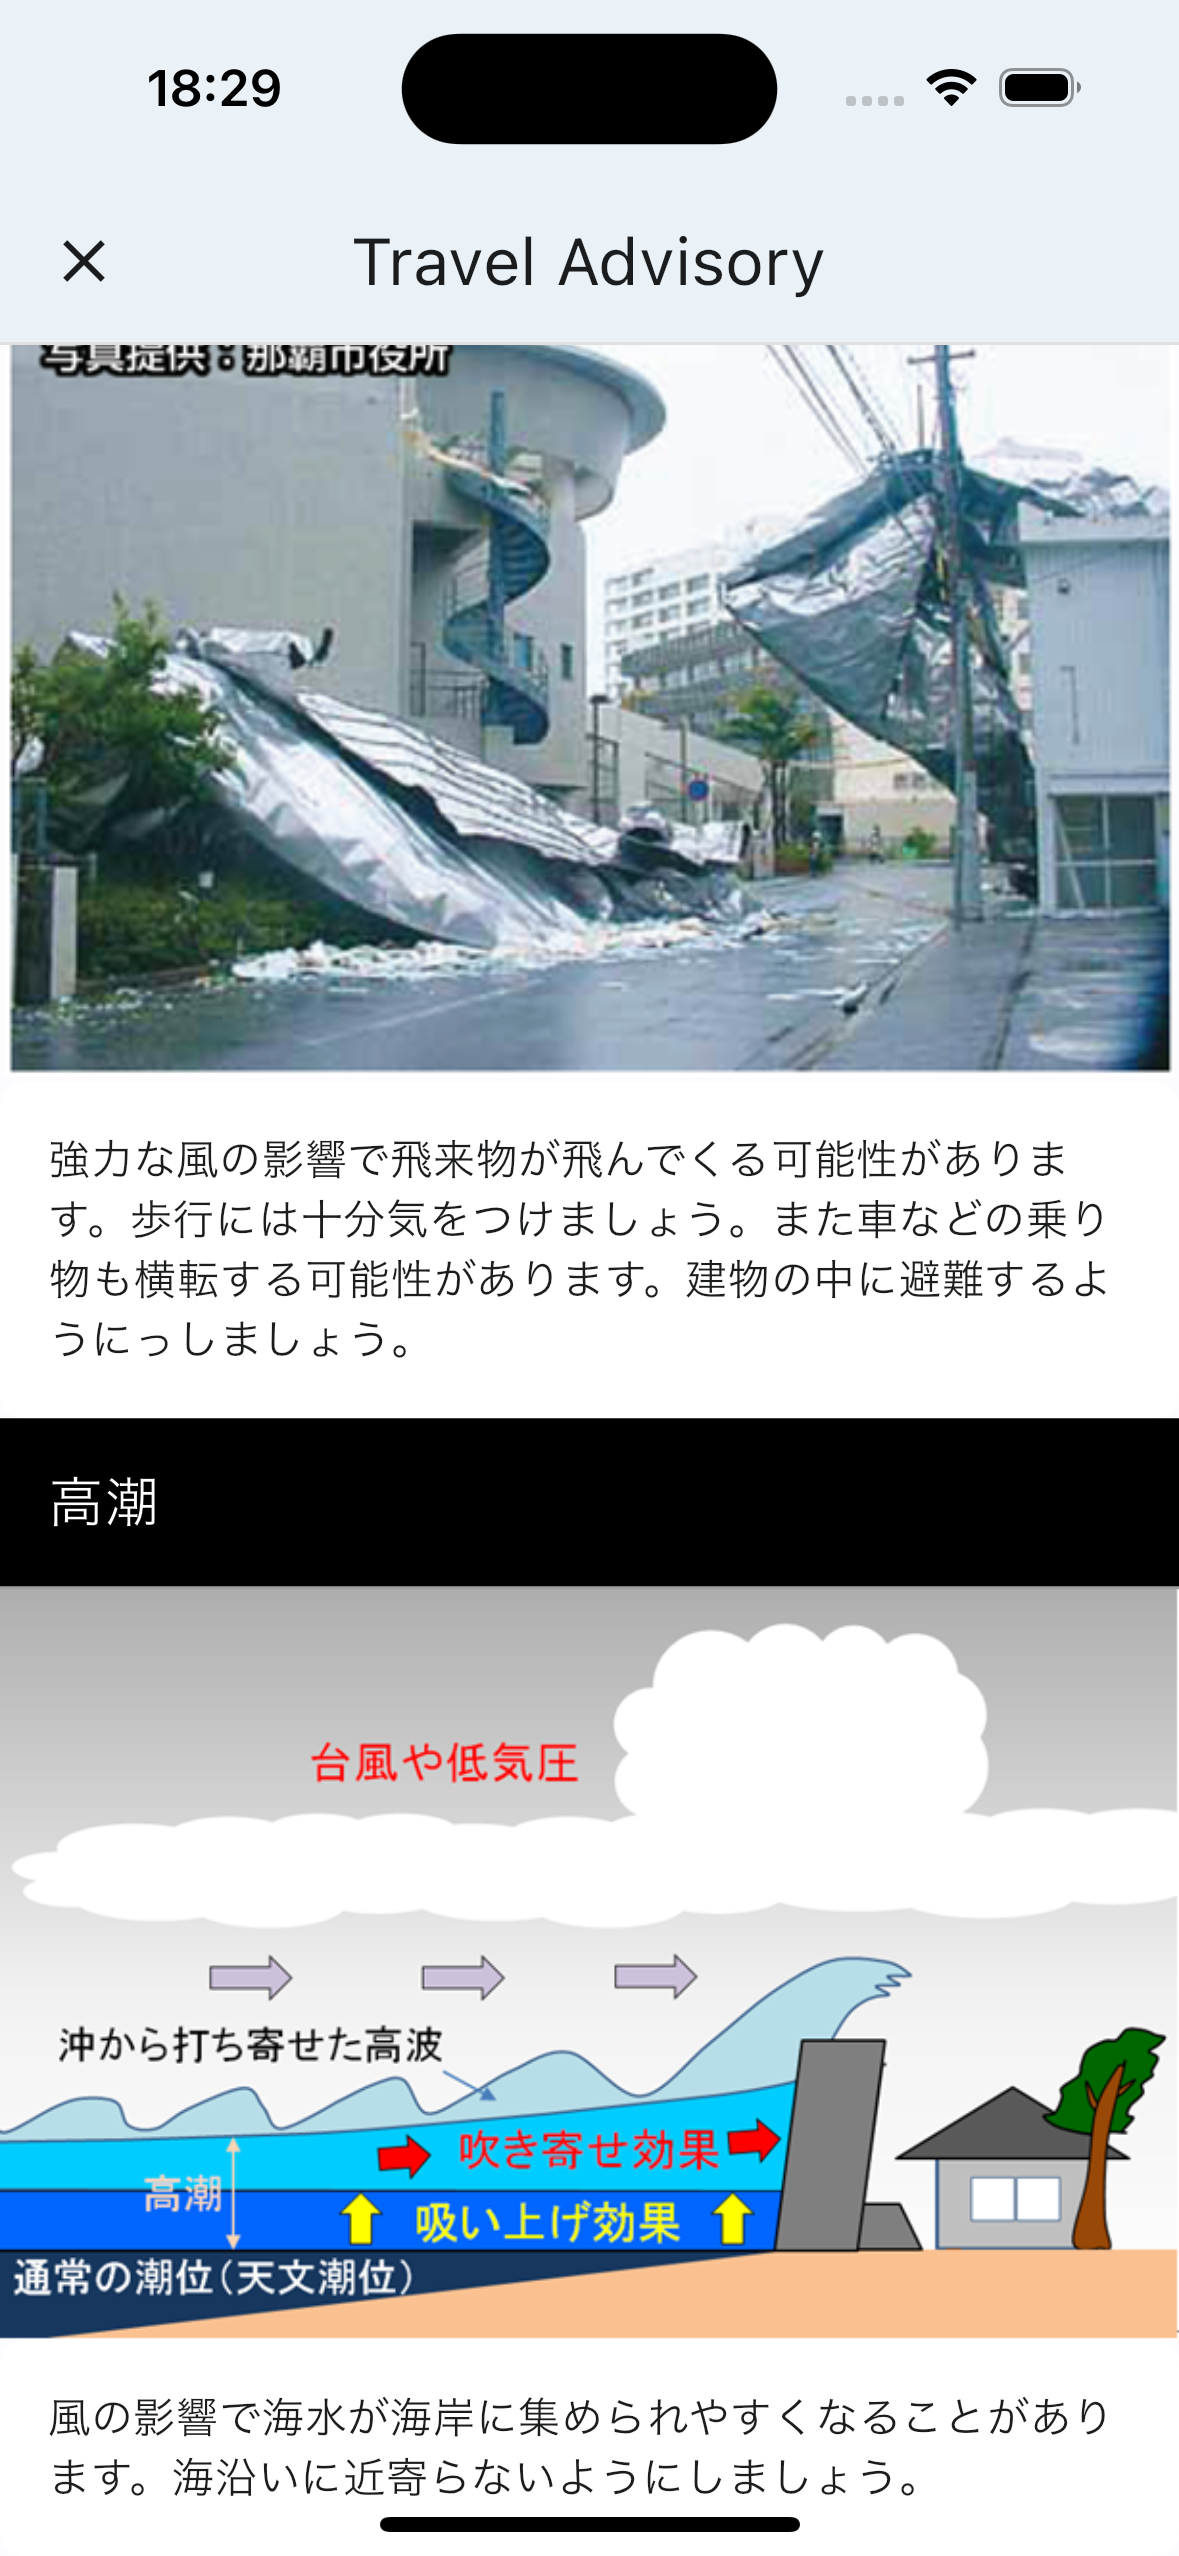
\includegraphics[height=10cm]{./fig/wind_stock_2.png}
    %\vspace{-3mm}
    \caption{風のストック情報提供画面2}
    \label{fig:rain_stock_2}
    %\vspace{2mm}
  \end{minipage}
\end{figure}

% \begin{figure}[H]
%   \centering
%   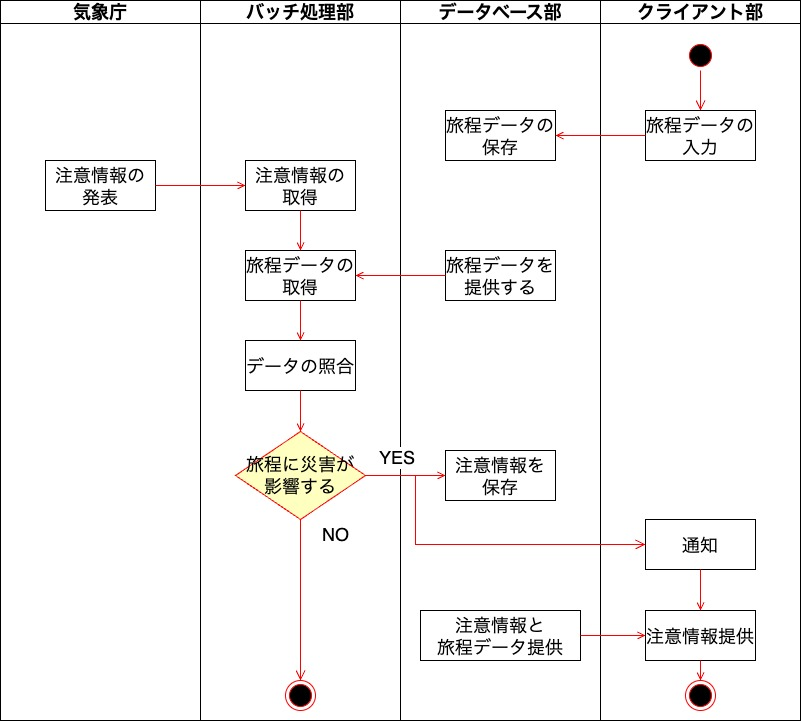
\includegraphics[height=8cm]{figure32.jpg}
%   %\vspace{-3mm}
%   \caption{場所データの注意情報提供画面の図}
%   \label{fig:activity}
%   %\vspace{2mm}
% \end{figure}

% \subsection {公共交通データの注意情報提供画面の図}

% \begin{figure}[H]
%   \centering
%   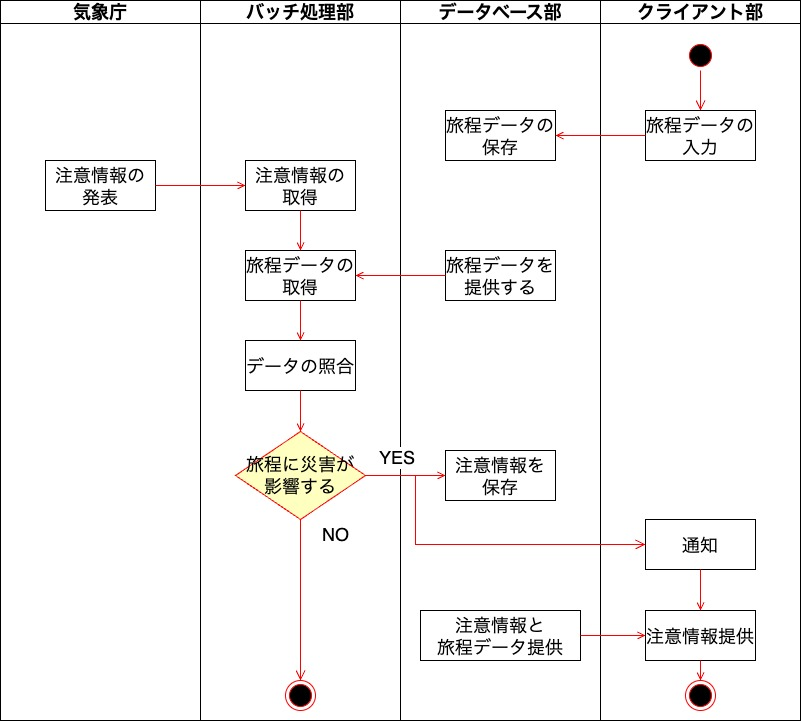
\includegraphics[height=8cm]{figure32.jpg}
%   %\vspace{-3mm}
%   \caption{公共交通データの注意情報提供画面の図}
%   \label{fig:activity}
%   %\vspace{2mm}
% \end{figure}

% \subsection {大雨に関するストック情報の提供画面の図}

% \begin{figure}[H]
%   \centering
%   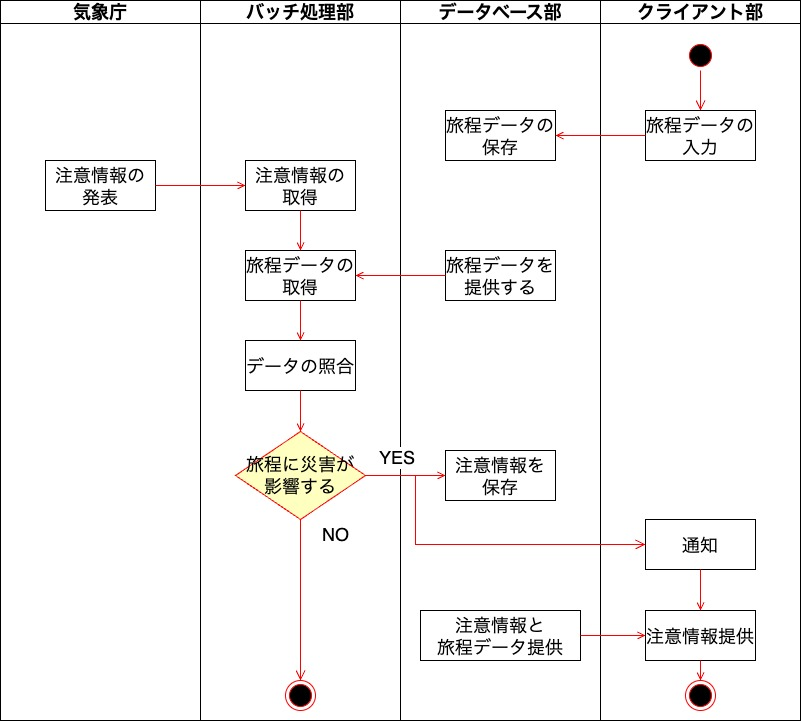
\includegraphics[height=8cm]{figure32.jpg}
%   %\vspace{-3mm}
%   \caption{大雨に関するストック情報の提供画面の図}
%   \label{fig:activity}
%   %\vspace{2mm}
% \end{figure}

% \subsection {風に関するストック情報の提供画面}

% \begin{figure}[H]
%   \centering
%   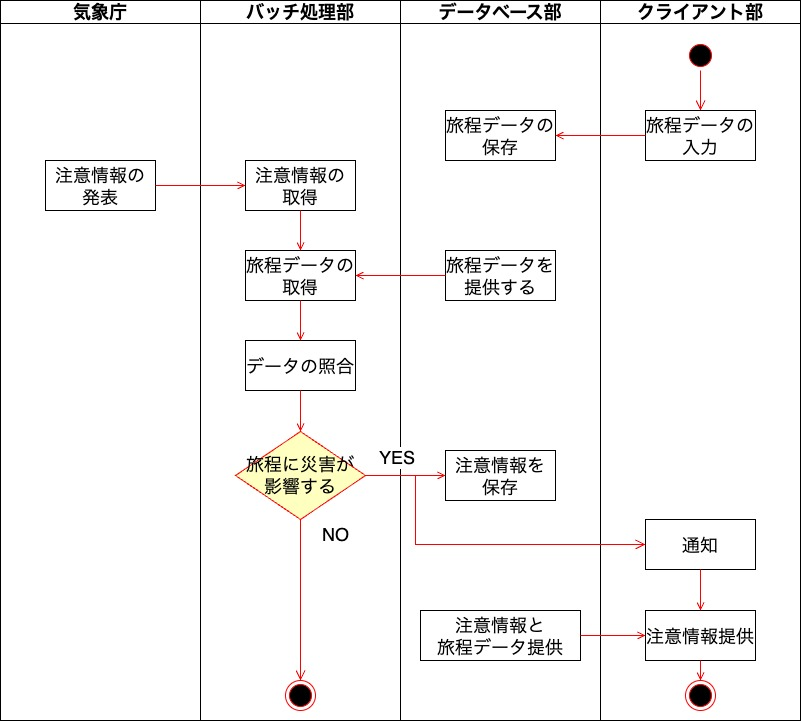
\includegraphics[height=8cm]{figure32.jpg}
%   %\vspace{-3mm}
%   \caption{風に関するストック情報の提供画面の図}
%   \label{fig:activity}
%   %\vspace{2mm}
% \end{figure}

%
\end{document} % 2章
\documentclass[a4paper,11pt,oneside,openany]{jsbook}
\usepackage{myjlabthesisstyle}
\daigaku{青山学院大学}
\gakubu{社会情報}
\gakka{社会情報学科}
\syubetsu{卒業論文}
\labname{宮治研究室}
\chiefexaminer{宮治~~裕~~教授}

%%%%%%%%%%%%%%%%%%%%%%%%%%%%%%%%%%%%%%%
% ここから先「ここまで個人設定」の範囲に
% 各自の固有の情報を記入して下さい
%%%%%%%%%%%%%%%%%%%%%%%%%%%%%%%%%%%%%%%
\nendo{2024年度}
\teisyutsu{2024年~~1月}
\snum{38122001}
\jname{黒川~~皇輝}
\thesistitle{訪日観光客を対象とした風水害注意情報提供システム} %タイトルを記入
%\thesissubtitle{\LaTeX の利用} %サブタイトルを記入 ない場合はコメントアウト
%\SUBTtrue %サブタイトル有りの場合 ない場合は,コメントアウト
\SUBTfalse %サブタイトル無しの場合 有る場合は,コメントアウト
%%%%%%%%%% ここまで個人設定 %%%%%%%%%%%%%%

\begin{document}

\chapter{\LaTeX の利用例}
本章では,\LaTeX の利用例について示す.
特に,基本的な記述方法,図の組み込み方,表の組み込み型について,具体例と共に解説する.

\section{基本的な使い方}
\LaTeX を利用する際に,最初に知っておくべきことは「スペース」や「改行」などが,エディタで入力したとおりにならないことと,キーボード上の記号の中には 「\%」 など,そのまま入力しただけでは出力できない文字が有るということである\footnote{ちなみに\%記号を表示したい場合は,「\verb+\%+」と入力する}.
これらのポイントは,電気通信大学 佐藤研究室による「TeXマニュアル」\cite{HTUlatex}にまとめられている.
%本パッケージにも,そのPDFファイルを texmanual.pdf として含めており,一読を推奨する.

以降,特に注意するポイントについてのみ記載する.
\subsection{章と節,節々}
章のタイトルには \verb+\chapter{}+,節のタイトルには \verb+\section{}+を利用する.
また,節の下のレベル(ここでは節々) のタイトルを記載するには \verb+\subsection{}+を利用する.
それぞれ,適切なフォーマットにて番号が付与されて,表示がなされる.

更に下のレベルは,\verb+subsubsection{}+を用いることができる.本スタイルパッケージでは,
このレベルにおいて番号を記載しないようにした.
したがって,このレベルを最小として論文を構成するようにして欲しい.

\subsection{改行と改段落}
\LaTeX では,改行には 「\verb+\\+」を,改段落には 「\verb+\par+」を利用する\footnote{改段落の場合には「\verb+\par+」を入れるのではなく,空白行を入れる方法を推奨するが,説明として記載している}.
改段落された後の段落は,自動的に一字下げされる.
また,連続する空白スペースは無視される.
つまり,エディタ上の改行は改行として反映されないし,半角英数字のスペースにて表現した改段落時の字下げは意味が無い\footnote{全角スペースにて表現した字下げは,一字分の空白に見えるが,行頭では無く文中の空白文字に見える}
.

一見不自由に見えるかもしれないが,この特性は論文を書く際に便利な機能である.
まず,論文を書く際に,意図的な改行を入れることはあまりない.
つまり改行の 「\verb+\\+」を使うことは,ほとんど無い.

逆に改段落は,論文を書く際には意識して頻繁に利用するが,段落が変わる位置に空白行を挿入すると,「\verb+\par+」と入力したことと同じ意味となる.
したがって,改段落には \verb+\par+を入れるのではなく,空白行を入れる方法を推奨する.

テキストエディタなどで文章を書く際のポイントと効果を以下にまとめる.
\begin{itemize}
\item 一文ずつエンターキーで改行しながら文章を記載する
\begin{itemize}
\item[・] 行がつながっていない方が,エディタ上の編集では効率的である
\item[・] エンターキーによる改行は,文章の見た目の改行ではない
\end{itemize}
\item 段落が変わる毎に空白行を挿入する
\begin{itemize}
\item[・] エディタ画面では,段落のまとまりがわかりやすい
\item[・] 文章のバランスや量などに気を配ることができる
\end{itemize}
\end{itemize}
上記ポイントを実践して記述した本書類の第1章の中身を以下に示す.

\begin{breakbox}
{\footnotesize
\begin{verbatim}
\chapter{はじめに}
本論文では,○○○を△△△することにより,□□を明らかとする研究について記述する.

まず,本研究をおこなう背景となった事柄について述べる.
次に,研究目的の詳細を記述した後,類似研究との相違や関連研究とのつながりについて解説する.
また,次章以降の本論文の構成についてその概略を述べる.

\section{背景}
研究の目的につながる背景事項を説明する.
その説明には,参考文献やデータを参照するように.

あまり詳しく書きすぎると,2章や3章などで書く内容が無くなったり重複したりしてしまうので,研究の目的の妥当性につながる程度の内容(詳細さ)でかまわない.

\section{研究目的}
背景によって,研究の大きな目的が導かれる.
その大きな目的を正確に定義した後,本研究にて実際にターゲットとする目的を詳細に記述する\footnote{大きな目的は1年間の研究ではカバーしきれない為}.

また,背景にて実際の詳細なターゲットの必要性を示した場合には,それの詳細な条件を記載する.
…
\end{verbatim}
}
\end{breakbox}

\section{図の挿入}
\LaTeX で図を挿入するというと,以前は EPS形式にする必要があった.
しかし,現在は PDF形式を扱うのが主流である.
したがって,自分で作図した場合は PDF形式にて出力保存するのが適当であろう.
なお,JPEGでもPNGでも挿入は可能なため,デジタルカメラの画像などは PDFに変換する必要は無い.

\subsection{挿入方法}
PDFが主流とはいえ,EPS形式の貼り付けが基本であるため,その方法をまず記述する.

図を入れたいところで以下の様に指定する.
\begin{breakbox}
{\small
\begin{verbatim}
\begin{figure}[htbp]
\centering
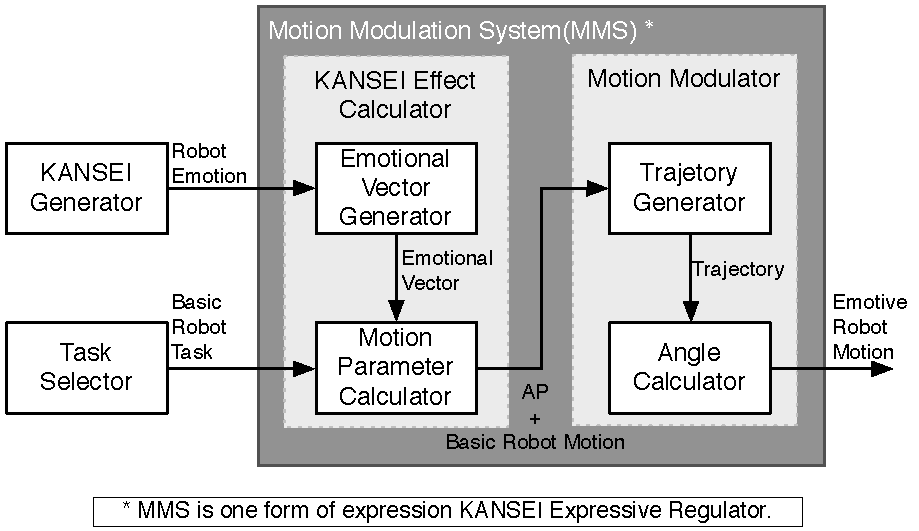
\includegraphics[height=7cm]{MMS.pdf}
\caption{MMSの内部構成}
\label{fig:mms}
\end{figure}
\end{verbatim}
}
\end{breakbox}

\verb+\caption{}+内には,図のタイトルや説明文章を書く(図番号の後ろの部分).
宮治研の場合は,必ず記載すること.
なお,このフォーマットを守る限り気にする必要は無いが,図のタイトルは図の下につけなければならない.

また,\verb+\label{}+は図番号を参照する際のラベルである(使い方は後述).
当然,図毎にラベルの名称を変えなければならない.

\begin{figure}[htb]
\centering
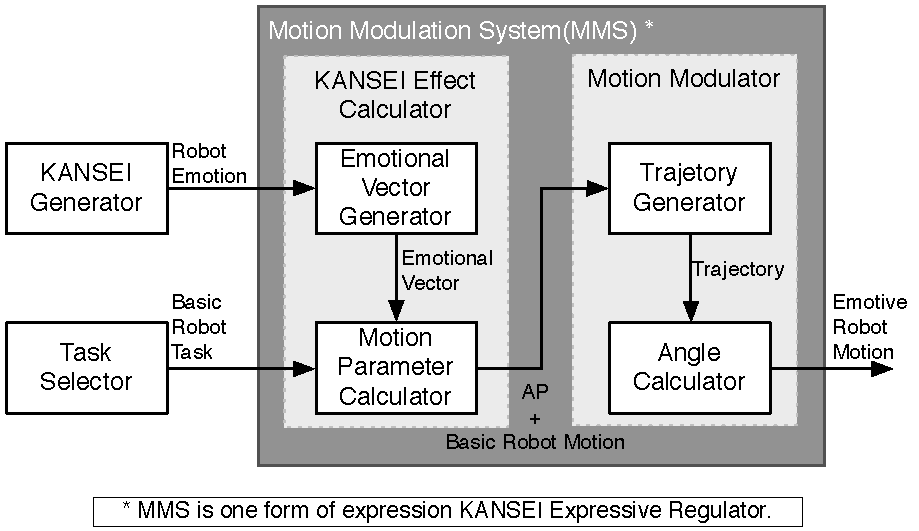
\includegraphics[height=7cm]{MMS.pdf}
%\vspace{-3mm}
\caption{PDF貼り付けの例:MMSの内部構成}
\label{fig:mms}
%\vspace{2mm}
\end{figure}

\subsection{図の位置の指定}
ここで,文章と文章の間などに図を入れたくなることがある.
これを制御する為の指定が,以下の部分である.
\begin{breakbox}
{\small
\begin{verbatim}
\begin{figure}[htbp]
\end{verbatim}
}
\end{breakbox}
「\verb+[htbp]+」の記載は,図を入れず場所の優先順位を「\verb+h+:ここに」「\verb+t+:ページ上部に」「\verb+b+:ページ下部に」「\verb+p+:1ページに」するという意味である.
状況に応じて,「\verb+[tb]+」「\verb+[ht]+」「\verb+[p]+」のように指定できる.
しかしながら,\LaTeX の場合,バランスがとれる位置に図を入れる為に,その出力位置を完全にはコントロールできないので,参照した場所より下に図が入っていれば良いぐらいの気持ちで良い.

ただし,今回のパッケージでは,float スタイルを組み込んでいる.
標準の \LaTeX にはない 「\verb+[H]+」オプションを使うことによって,強制的にその場に入れることができる.

\begin{breakbox}
{\small
\begin{verbatim}
\begin{figure}[H]
\centering
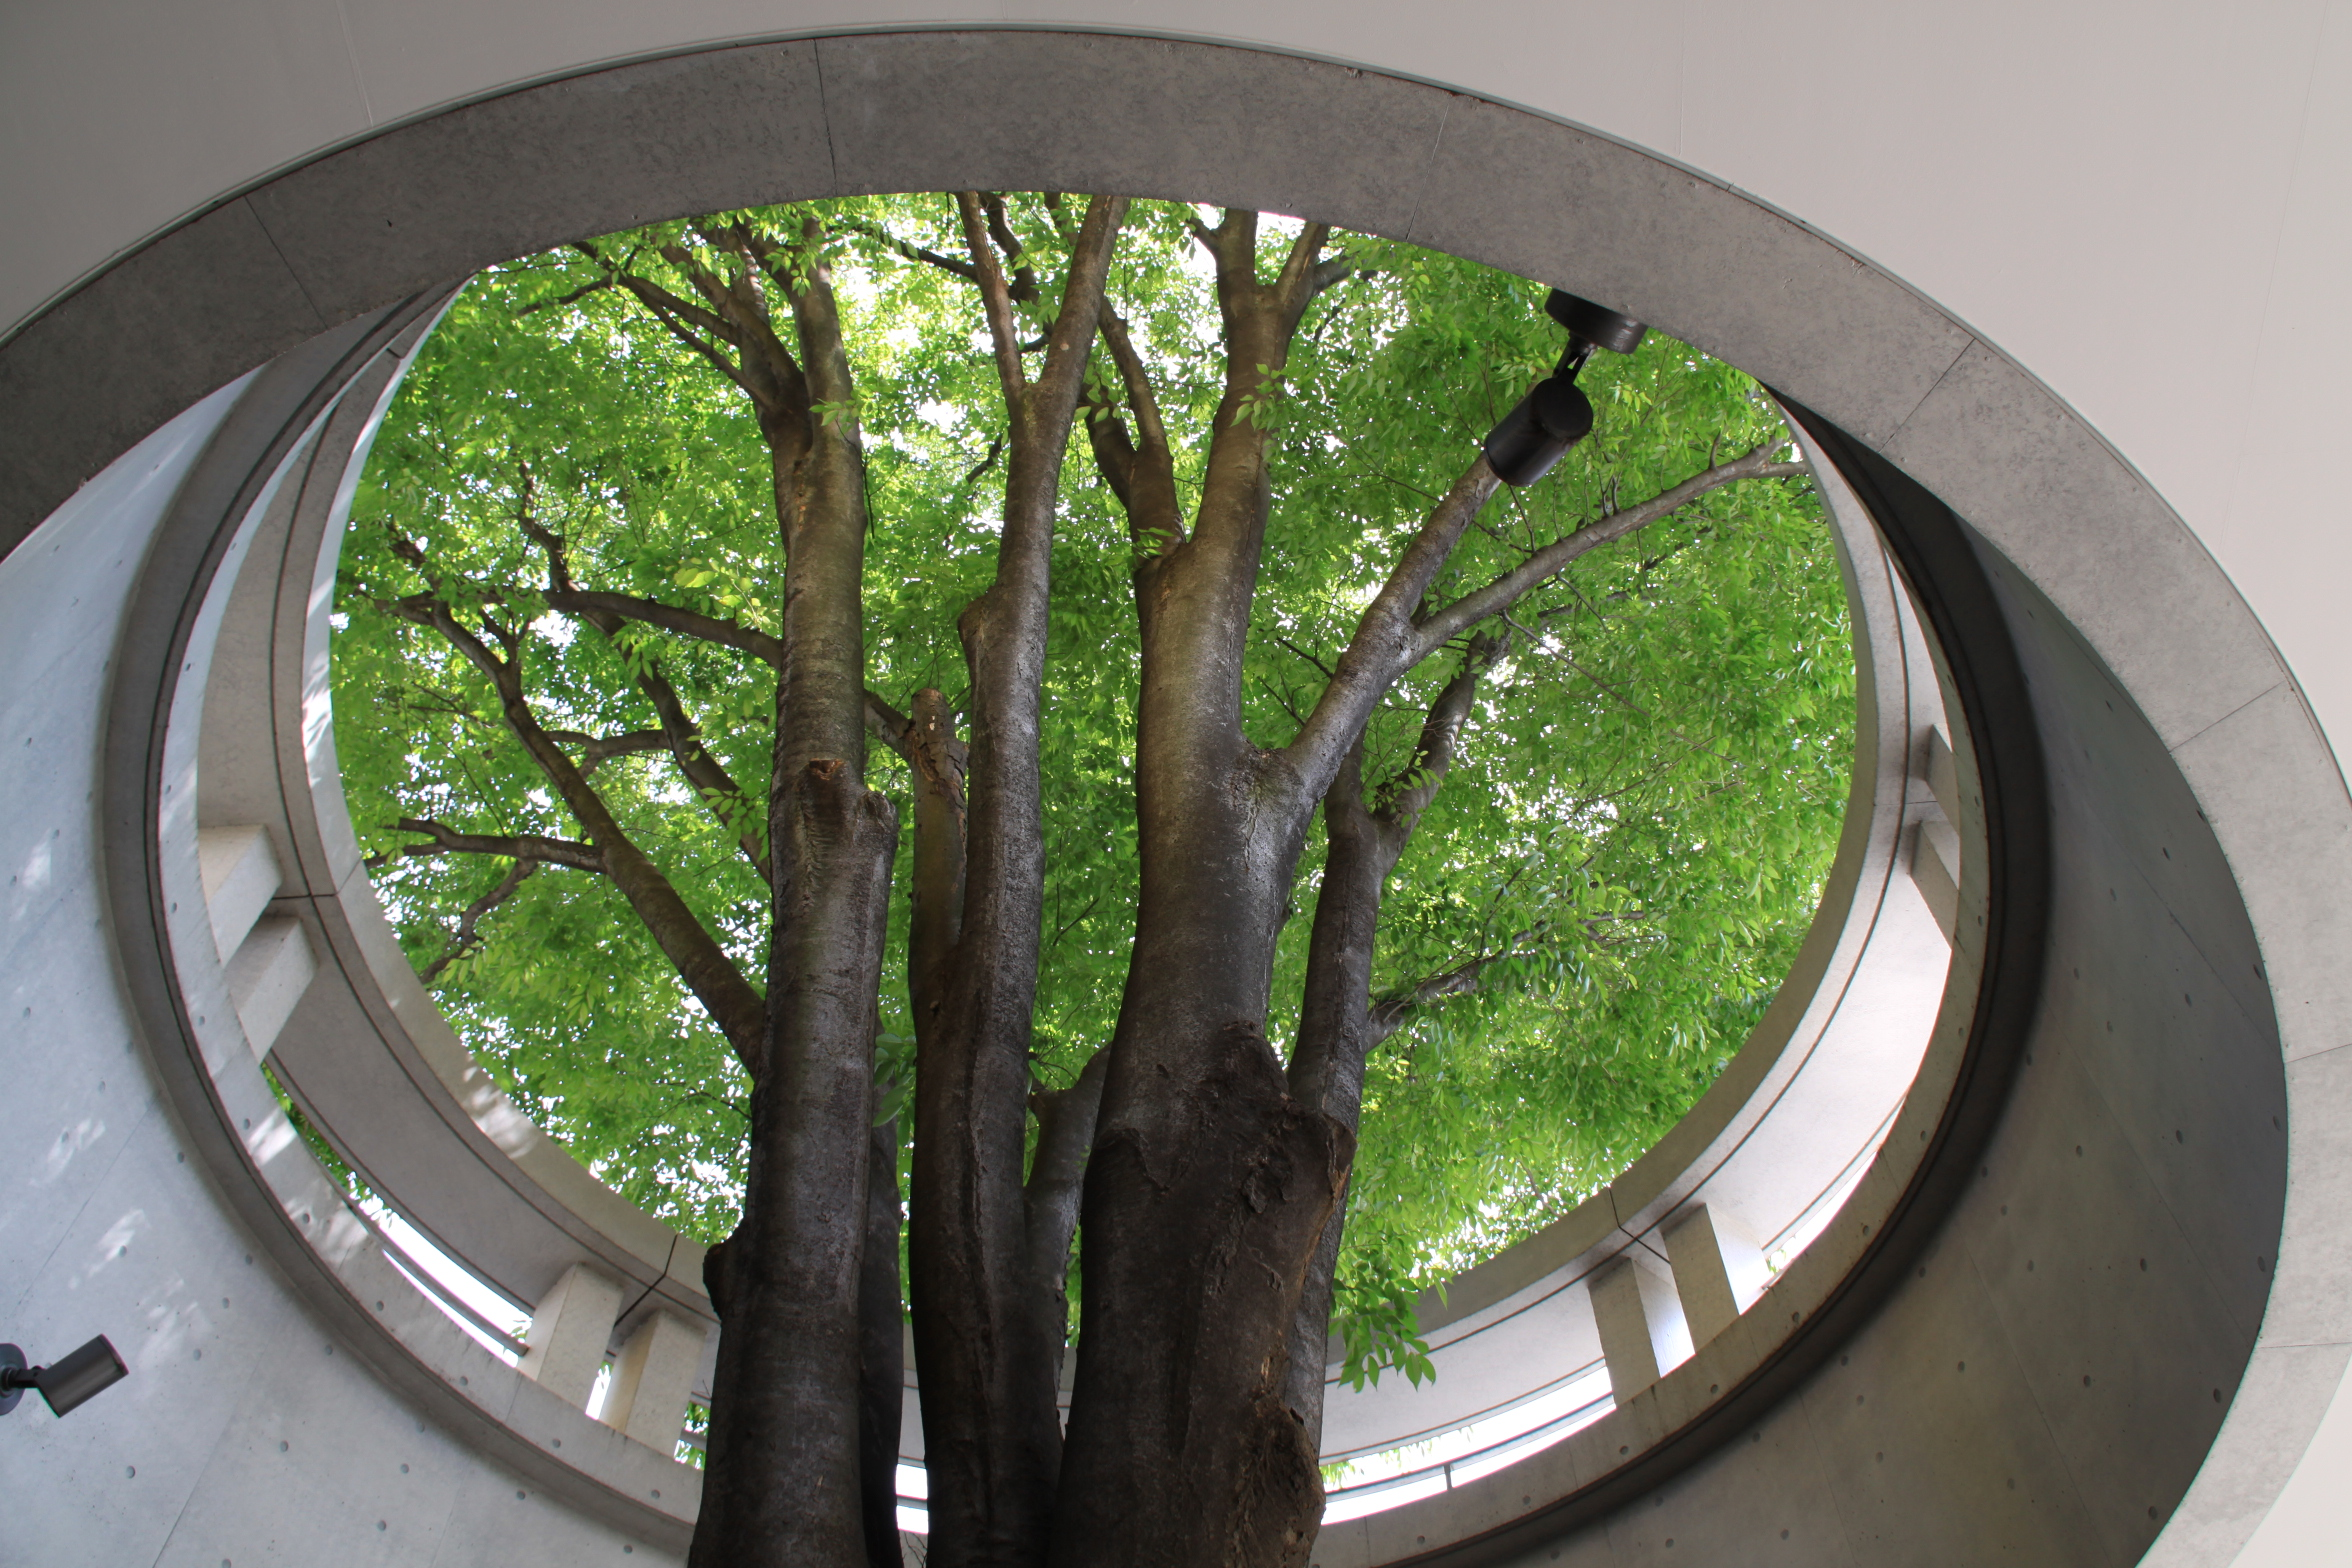
\includegraphics[height=5cm]{DEF059.jpg}
\caption{JPEG貼り付けの例:学内の写真}
\label{fig:sagamiC}
\end{figure}
\end{verbatim}
}
\end{breakbox}

\begin{figure}[H]
\centering
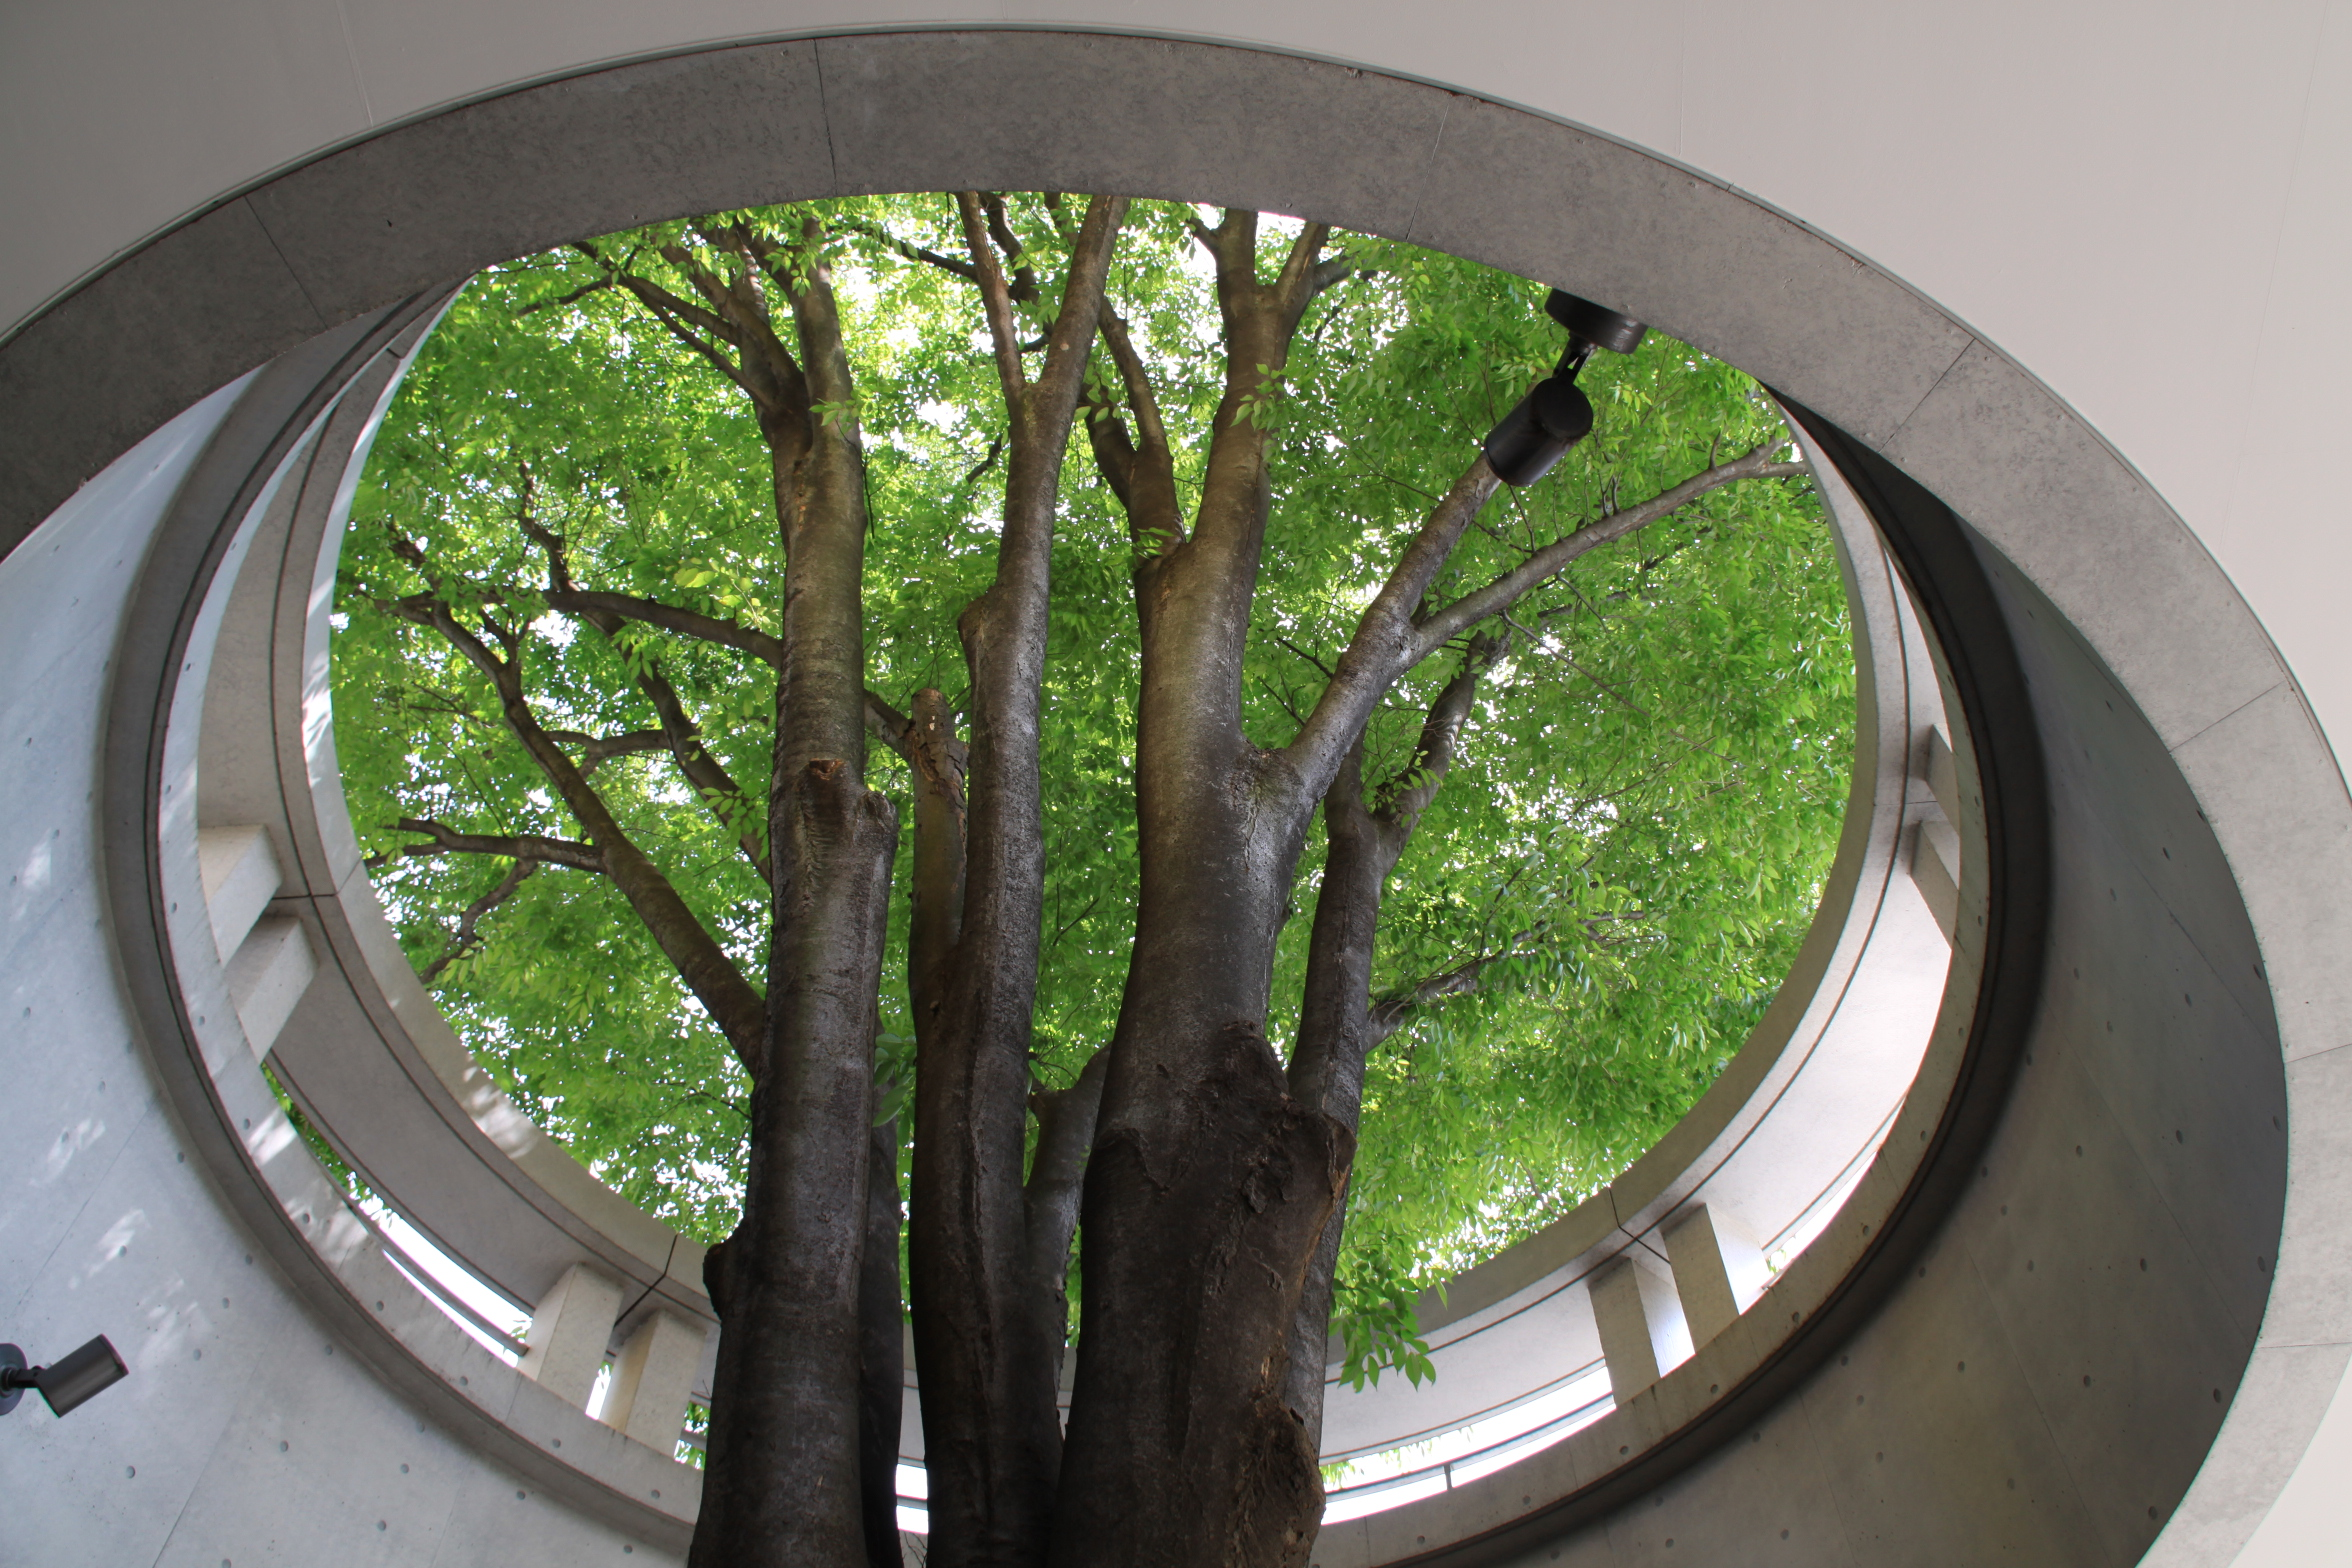
\includegraphics[height=5cm]{DEF059.jpg}
%\vspace{-3mm}
\caption{JPEG貼り付けの例:学内の写真}
\label{fig:sagamiC}
%\vspace{2mm}
\end{figure}

\subsection{図の参照}
図の挿入の際に(先ほど)記入した \verb+\label{fig:mms}+ は,図番号を参照したい際に指定するラベルを設定していた.
これを参照するには,「\verb+図 \ref{fig:mms}+」と指定すれば,図 \ref{fig:mms} の様に出力される.

\subsection*{補足:PDF, JPEG, PNG形式の場合の注意}
図の大きさを知らせる xbbファイルが必要になる.
これは,extractbbコマンドにて生成可能である.
本パッケージでは,\verb+mklatex.bat+ ファイルにて自動生成するように設定したため,あまり気にせず正しいファイル名のみ指定すれば良い.

\section{表の挿入}
本節では、表の挿入に関して記述する.
また、表の作成方法や書式の変更方法についても実例を元に解説する.

\subsection{表の作成と変換方法}
馴れてくれば \LaTeX の命令を直接記述して表を作るのは容易だが、最初の内は手こずるかもしれない.
ここでは論文に用いる一般的な表を元に、一番簡単と思われる作成と貼り付けの方法を記載する.

\subsubsection{表の作成}
図\ref{fig:tableFinish}の様な表を仕上がりのイメージと仮定する.
\begin{figure}[H]
\centering
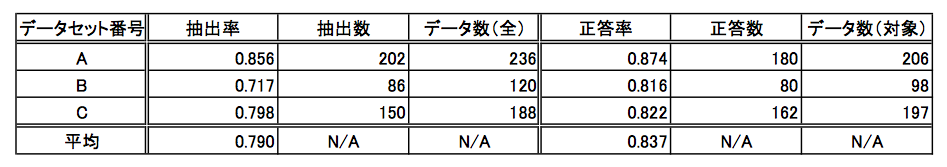
\includegraphics[width=14cm]{tableFinishImage.png}
\vspace{-3mm}
\caption{貼り付けたい表の仕上がりのイメージ}
\label{fig:tableFinish}
%\vspace{2mm}
\end{figure}

まず、Excel等で表を作成しておく.
\begin{figure}[H]
\centering
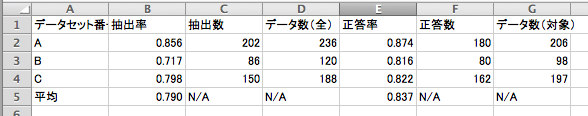
\includegraphics[width=14cm]{excelTable.png}
\vspace{-3mm}
\caption{Excelで作成した表}
\label{fig:excelTable}
%\vspace{2mm}
\end{figure}

\subsubsection{表の変換}
CSV2TeX(\url{http://naisodewafurenu.web.fc2.com/csv2tex.html})に接続する.
\begin{figure}[H]
\centering
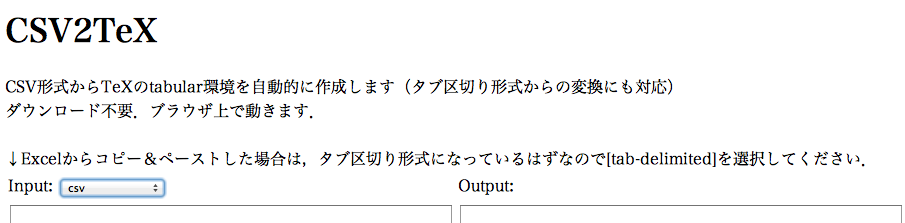
\includegraphics[width=12cm]{csv2tex.png}
\vspace{-3mm}
\caption{CSV2TeXのサイト}
\label{fig:csv2tex}
%\vspace{2mm}
\end{figure}

Inputのプルダウンメニューから「tab-delimited」を選択する.
\begin{figure}[H]
\centering
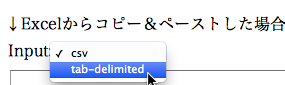
\includegraphics[width=6.5cm]{inputTypeChange.png}
%\vspace{-3mm}
\caption{入力方式の変更}
\label{fig:inputTypeChange}
%\vspace{2mm}
\end{figure}



その直下のボックスにExcelの表をペーストし、「CONVERT」ボタンを押下する.
Outputのボックス内に \LaTeX の表組みの命令が埋め込まれたデータが出力される.
%\begin{figure}[htb]
%\begin{center}
%\includegraphics[height=4cm]{sc02.png}
%\vspace{-3mm}
%\end{center}
%\caption{Excelの表の例}
%\label{fig:excel}
%\vspace{2mm}
%\end{figure}
\begin{figure}[htb]
\centering
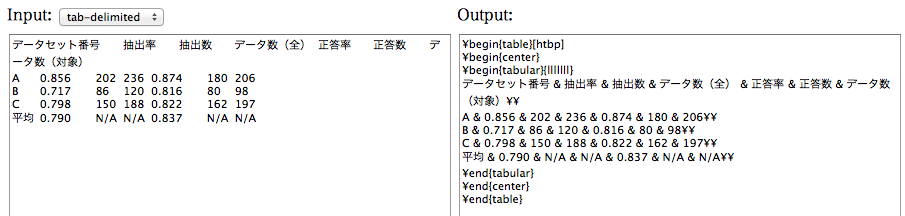
\includegraphics[width=14cm]{convertTable.png}
%\vspace{-3mm}
\caption{CSV2TeXの操作例}
\label{fig:convertTable}
%\vspace{2mm}
\end{figure}

これをtexファイルに貼り付ける.
\begin{breakbox}
{\small
\begin{verbatim}
\begin{table}[htbp]
\begin{center}
\begin{tabular}{lllllll}
データセット番号 & 抽出率 & 抽出数 & データ数(全) & 正答率 & 正答数 & データ数(対象)\\
A & 0.856 & 202 & 236 & 0.874 & 180 & 206\\
B & 0.717 & 86 & 120 & 0.816 & 80 & 98\\
C & 0.798 & 150 & 188 & 0.822 & 162 & 197\\
平均 & 0.790 & N/A & N/A & 0.837 & N/A & N/A\\
\end{tabular}
\end{center}
\end{table}
\end{verbatim}
}
\end{breakbox}

\subsubsection{表の修正}
このままでは、キャプションとラベルが不足しているので、それらの情報を足すことにする.
また、現在の\LaTeX では、図表内において \verb+\begin{center}+と\verb+\end{center}+の代わりに\verb+\centering+命令を使うことが推奨されている為、それも変更する.

まず、命令の上部
\begin{breakbox}
{\small
\begin{verbatim}
\begin{table}[htbp]
\begin{center}
\begin{tabular}{lllllll}
\end{verbatim}
}
\end{breakbox}
に対して、以下の様に修正する.
\begin{breakbox}
{\small
\begin{verbatim}
\begin{table}[htbp]
\caption{実験1の結果}
\centering
\begin{tabular}{lllllll}
\end{verbatim}
}
\end{breakbox}

また、命令下部
\begin{breakbox}
{\small
\begin{verbatim}
\end{tabular}
\end{center}
\end{table}
\end{verbatim}
}
\end{breakbox}
に対して、以下の様に修正する.
\begin{breakbox}
{\small
\begin{verbatim}
\end{tabular}
\label{table:resultEx1}
\end{table}
\end{verbatim}
}
\end{breakbox}


その出力を、表 \ref{table:resultEx1a}に示す.
\begin{table}[H]
\caption{実験1の結果}
\centering
\begin{tabular}{lllllll}
データセット番号 & 抽出率 & 抽出数 & データ数(全) & 正答率 & 正答数 & データ数(対象)\\
A & 0.856 & 202 & 236 & 0.874 & 180 & 206\\
B & 0.717 & 86 & 120 & 0.816 & 80 & 98\\
C & 0.798 & 150 & 188 & 0.822 & 162 & 197\\
平均 & 0.790 & N/A & N/A & 0.837 & N/A & N/A\\
\end{tabular}
\label{table:resultEx1a}
\end{table}


\subsection{横罫線の設定}
横罫線には「\verb+\hline+」命令を利用する.
横罫線を引きたい場所で、\verb+\hline+を入力する.二重線を引きたい場合には、\verb+\hline \hline+と記述すれば良い.

例えば、以下の命令を出力すると表\ref{table:resultEx1b}の様に出力される.
\begin{breakbox}
{\small
\begin{verbatim}
\begin{tabular}{lllllll}
\hline
データセット番号 & 抽出率 & 抽出数 & データ数(全) & 正答率 & 正答数 & データ数(対象)\\ \hline \hline
A & 0.856 & 202 & 236 & 0.874 & 180 & 206\\ \hline
B & 0.717 & 86 & 120 & 0.816 & 80 & 98\\ \hline
C & 0.798 & 150 & 188 & 0.822 & 162 & 197\\ \hline \hline
平均 & 0.790 & N/A & N/A & 0.837 & N/A & N/A\\ \hline
\end{tabular}
\end{verbatim}
}
\end{breakbox}

\begin{table}[H]
\caption{実験1の結果}
\centering
\begin{tabular}{lllllll}
\hline
データセット番号 & 抽出率 & 抽出数 & データ数(全) & 正答率 & 正答数 & データ数(対象)\\ \hline \hline
A & 0.856 & 202 & 236 & 0.874 & 180 & 206\\ \hline
B & 0.717 & 86 & 120 & 0.816 & 80 & 98\\ \hline
C & 0.798 & 150 & 188 & 0.822 & 162 & 197\\ \hline \hline
平均 & 0.790 & N/A & N/A & 0.837 & N/A & N/A\\ \hline
\end{tabular}
\label{table:resultEx1b}
\end{table}

「\verb+\begin{tabular}+」の次の行の「\verb+\hline+」だけが記載されている行は、一番上の横罫線を示す.
また表の一行目(見出し)の最後の部分をみると、改行「\verb+\\+」をし、その後に2回罫線を引く「\verb+\hline \hline+」命令が書かれている為、二重罫線が表示されている.
その他の行は、必要に応じて1回または2回の「\verb+\\ \hline+」が記載されている.

\subsection{表内の基本部分の表示位置の変更}
表内の文字の表示位置を制御している命令は、\verb+\begin{tablar}{lllllll}+
の部分である.
この\verb+{lllllll}+は、表が7列(\verb+l+が7個ある)でできており、それらを「\verb+l+:左寄せ」で表示することを意味している.

表内の表示位置の修正としては、表の大部分を占める部分(2行目から4行目のデータが入っている部分)を元に、位置の指定をしていく.
まず、1列目「AとBとC」とかかれた部分の部分は文字情報なので、センタリング「\verb+c+」にする.
また、2列目から7列目は、数値データが入っていることから、右寄せ「\verb+r+」にする.
したがって、位置の指定は、\verb+\begin{tablar}{crrrrrr}+ とすれば良い.
以上の修正をした表を表 \ref{table:resultEx1c}に示す.
\begin{table}[H]
\caption{実験1の結果}
\centering
\begin{tabular}{crrrrrr}
\hline
データセット番号 & 抽出率 & 抽出数 & データ数(全) & 正答率 & 正答数 & データ数(対象)\\ \hline \hline
A & 0.856 & 202 & 236 & 0.874 & 180 & 206\\ \hline
B & 0.717 & 86 & 120 & 0.816 & 80 & 98\\ \hline
C & 0.798 & 150 & 188 & 0.822 & 162 & 197\\ \hline \hline
平均 & 0.790 & N/A & N/A & 0.837 & N/A & N/A\\ \hline
\end{tabular}
\label{table:resultEx1c}
\end{table}

欧文の論文の場合には、表の縦線を入れないことが多い為、以上で表が完成したと考えて良い.

和文の論文に見られる様に、表の縦線を入れこともできるが、縦線を入れたが為に見出しの位置などが気になり、さらなる調整が必要になることが多い.通常は、ここまでで良いだろう.

\subsection{表の参照}
表の環境でもラベルが設定でき、図と同様の手法で参照することができる.例えば、表 \ref{table:resultEx1a}の命令内では、「\verb+\label{table:resultEx1a}+」と設定されているため、「\verb+表 \ref{table:resultEx1a}+」の様に指定すれば 表 \ref{table:resultEx1a} と参照できる.

\subsection{表の位置の設定}
表の位置の設定は、図の位置の設定と同様「\verb+[htbp]+」の様な指定ができる.である.また、floatパッケージを読み込んでいる為、強制的にその場所に出力する「\verb+[H]+」も利用できる.

\subsection{縦罫線の設定と表内見出しなどの位置変更}
縦方向罫線の入れ方と、それに伴う見出しなどの表示位置変更方法について記載する.

\subsubsection{縦罫線の設定}
列の要素のどこに縦罫線を引くのかを「\verb+|+」を使って指示する.
また、2重罫線は「\verb+||+」を利用する.
例えば、今回の仕上がりのイメージでは、1列目と4列目の右が2重罫線、残りと外側が通常の縦罫線だったので、
「\verb+\begin{tabular}{|c||r|r|r||r|r|r|}+」と書く.
\begin{table}[H]
\caption{実験1の結果}
\centering
\begin{tabular}{|c||r|r|r||r|r|r|}
\hline
データセット番号 & 抽出率 & 抽出数 & データ数(全) & 正答率 & 正答数 & データ数(対象)\\ \hline \hline
A & 0.856 & 202 & 236 & 0.874 & 180 & 206\\ \hline
B & 0.717 & 86 & 120 & 0.816 & 80 & 98\\ \hline
C & 0.798 & 150 & 188 & 0.822 & 162 & 197\\ \hline \hline
平均 & 0.790 & N/A & N/A & 0.837 & N/A & N/A\\ \hline
\end{tabular}
\label{table:resultEx1d}
\end{table}

\subsubsection{表内の見出し行などの部分の表示位置の変更}
表の1行目(ラベル部分)は、2行目から4行目と異なり、それぞれの列を説明する言葉が書かれている.
これは、表内右寄せでは無く、センタリングとしたい.

このように書かれている部分を(表示の関係から行を折り返している)
\begin{breakbox}
{\small
\begin{verbatim}
\begin{tabular}{|c||r|r|r||r|r|r|}
\hline
データセット番号 & 抽出率
  & 抽出数 & データ数(全)
  & 正答率 & 正答数
  & データ数(対象)\\ \hline \hline
\end{verbatim}
}
\end{breakbox}
以下の様に変更する.
\begin{breakbox}
{\small
\begin{verbatim}
\begin{tabular}{|c||r|r|r||r|r|r|}
\hline
\multicolumn{1}{|c||}{データセット番号} & \multicolumn{1}{c|}{抽出率}
  & \multicolumn{1}{c|}{抽出数} & \multicolumn{1}{c||}{データ数(全)}
  & \multicolumn{1}{c|}{正答率} & \multicolumn{1}{c|}{正答数}
  & \multicolumn{1}{c|}{データ数(対象)} \\ \hline \hline
\end{verbatim}
}
\end{breakbox}

なお、命令を見て分かるように \verb+multicolmun+命令を利用する際には、罫線情報は再度指定する必要がある.

また、最後の行は「N/A」の文字は表内でセンタリングとしたい.

同様にこのように書かれている部分を(表示の関係から行を折り返している)
\begin{breakbox}
{\small
\begin{verbatim}
平均 & 0.790
  & N/A & N/A
  & 0.837 & N/A
  & N/A\\ \hline
\end{tabular}
\end{verbatim}
}
\end{breakbox}
以下の様に修正する.
\begin{breakbox}
{\small
\begin{verbatim}
平均 & 0.790
  & \multicolumn{1}{c|}{N/A} & \multicolumn{1}{c||}{N/A}
  & 0.837 & \multicolumn{1}{c|}{N/A}
  & \multicolumn{1}{c|}{N/A} \\ \hline
\end{tabular}
\end{verbatim}
}
\end{breakbox}

以上の修正を施すと、表\ref{table:resultEx1e}の様に出力される.

\begin{table}[H]
\caption{実験1の結果}
\centering
\begin{tabular}{|c||r|r|r||r|r|r|}
\hline
\multicolumn{1}{|c||}{データセット番号} & \multicolumn{1}{c|}{抽出率}
  & \multicolumn{1}{c|}{抽出数} & \multicolumn{1}{c||}{データ数(全)}
  & \multicolumn{1}{c|}{正答率} & \multicolumn{1}{c|}{正答数}
  & \multicolumn{1}{c|}{データ数(対象)} \\ \hline \hline
A & 0.856 & 202 & 236 & 0.874 & 180 & 206\\ \hline
B & 0.717 & 86 & 120 & 0.816 & 80 & 98\\ \hline
C & 0.798 & 150 & 188 & 0.822 & 162 & 197\\ \hline
平均 & 0.790
  & \multicolumn{1}{c|}{N/A} & \multicolumn{1}{c||}{N/A}
  & 0.837 & \multicolumn{1}{c|}{N/A}
  & \multicolumn{1}{c|}{N/A} \\ \hline
\end{tabular}
\label{table:resultEx1e}
\end{table}

\section{参考文献と参照}
参照命令に応じて拡張子が bib であるファイルから情報が読み取られ,適切な番号が割り振られ,その番号順に参考文献が作成される.
例えば,「湖上ら\cite{Kogami2009}は,人間共生型ロボットの感性出力に関する研究を行った.」という文章において,参照の命令は「\verb+\cite{Kogami2009}+」の様に記載されている.
これで参考文献の出力順に応じた番号が自動的に割り振られ,参考文献のページに適切なフォーマットにて出力がなされる\cite{miyaji2010}.

この引用のラベルは,myrefs.bib ファイルにて,以下の様に記載されている.
\begin{breakbox}
{\small
\begin{verbatim}
@article{Kogami2009,
 author = "湖上 潤 and 宮治 裕 and 富山 健",
 title = "人間共生ロボットにおける擬似感性システムの構築と評価",
 journal = "日本感性工学会論文誌",
 pages = "601-609",
 month = sep,
 year = 2009,
}
\end{verbatim}
}
\end{breakbox}
この \BibTeX の書式は,全て各自で記述しても構わないが,一般的な論文をダウンロードするサイトにおいて出力することができるようになっており,それを利用して良い.

上記例は論文に関する情報であるが,書籍(の一部)\cite{WelfareJapan},書籍\cite{Nakata2010},予稿集\cite{Miyaji2003ROMAN},その他(Webサイトなど)\cite{HTUlatex}で参考文献欄に載せる情報は異なる.
それぞれの書式を記載しておいたので,各自で myrefs.bib ファイルを参照して欲しい.


%
\end{document} % 3章
\documentclass[a4paper,11pt,oneside,openany]{jsbook}
\usepackage{myjlabthesisstyle}
\daigaku{青山学院大学}
\gakubu{社会情報}
\gakka{社会情報学科}
\syubetsu{卒業論文}
\labname{宮治研究室}
\chiefexaminer{宮治~~裕~~教授}

%%%%%%%%%%%%%%%%%%%%%%%%%%%%%%%%%%%%%%%
% ここから先「ここまで個人設定」の範囲に
% 各自の固有の情報を記入して下さい
%%%%%%%%%%%%%%%%%%%%%%%%%%%%%%%%%%%%%%%
\nendo{2024年度}
\teisyutsu{2024年~~1月}
\snum{38122001}
\jname{黒川~~皇輝}
\thesistitle{訪日観光客を対象とした風水害注意情報提供システム} %タイトルを記入
%\thesissubtitle{\LaTeX の利用} %サブタイトルを記入 ない場合はコメントアウト
%\SUBTtrue %サブタイトル有りの場合 ない場合は,コメントアウト
\SUBTfalse %サブタイトル無しの場合 有る場合は,コメントアウト
%%%%%%%%%% ここまで個人設定 %%%%%%%%%%%%%%

\begin{document}

\chapter{おわりに}
本章では本研究のまとめと今後の展望について述べる.

\section{まとめ}
本研究は気象庁が発表する早期注意情報を利用し,訪日観光客が風水害の影響を受ける前に情報を提供することで,防災行動を促す効果があることを明らかにする研究であった.
この研究をおこなった背景は,訪日観光客が台風などの風水害の現象を想起することが難しく,現状の情報提供方法は日本住民向けであるため,訪日観光客に理解し難いことであった.
原因はストック情報が既知でなく,フロー情報を理解できないことであった.
ストック情報とはこれまでの教育や訓練などで人に蓄積された災害に関する情報である.
フロー情報はある特定の災害に対する災害についての説明と避難の呼びかけの情報である.

その問題に対して,訪日観光客の旅行計画に基づいて訪日中に災害の影響を受けるか監視し,影響がある場合ストック情報とフロー情報を提供するシステムを提案した.
新規性は情報提供するタイミングが余裕を持っておこなうことと,ストック情報を知らなくても理解しやすい情報を提供していることである.

気象庁が提供している天気予報の情報とシステムが提供する情報を比較することで,比較実験をおこなった.
実験参加者は全て日本人である.
防護動機理論という理論に基づいて,指標は脅威評価とした.
アンケート調査をおこない,脅威評価を構成する災害の深刻さに対する認知と災害発生の確率に対する認知についての評価を収集した.
過去の災害の情報から,実験用の旅程を2つ作成した.1日先に災害の可能性が認められる旅程と2日先に災害の可能性が認められる旅程である.
実験の結果,どちらの旅程においても天気予報から情報を得た実験参加者より,システムをから情報を得た実験参加者の脅威評価の方が高いと判明した.
さらに,システムはより未来の旅行日程に対して天気予報よりも脅威評価を高まらせる効果がある.
したがって,システムは天気予報と比較するとより高い脅威評価を与える効果があり,事前に防災行動を促すことが見込める.

\section{今後の展望}
今回の実験は日本人を対象としておこなったので,訪日観光客に防災行動を促すという目的を達成できたとは言えない.
今後の展望として,外国人を対象とした評価実験をおこなう必要がある.
また,システムで提供する情報も外国語化する必要がある.
そして,提供する情報についても文献から確認できた情報のみに基づいて作成されたので,訪日観光客に使用してもらった感想を聞き,洗練していきたい.
%
\end{document} % 4章
\documentclass[a4paper,11pt,oneside,openany]{jsbook}
\usepackage{myjlabthesisstyle}
\daigaku{青山学院大学}
\gakubu{社会情報}
\gakka{社会情報学科}
\syubetsu{卒業論文}
\labname{宮治研究室}
\chiefexaminer{宮治~~裕~~教授}

%%%%%%%%%%%%%%%%%%%%%%%%%%%%%%%%%%%%%%%
% ここから先「ここまで個人設定」の範囲に
% 各自の固有の情報を記入して下さい
%%%%%%%%%%%%%%%%%%%%%%%%%%%%%%%%%%%%%%%
\nendo{2024年度}
\teisyutsu{2024年~~1月}
\snum{38122001}
\jname{黒川~~皇輝}
\thesistitle{訪日観光客を対象とした風水害注意情報提供システム} %タイトルを記入
%\thesissubtitle{\LaTeX の利用} %サブタイトルを記入 ない場合はコメントアウト
%\SUBTtrue %サブタイトル有りの場合 ない場合は,コメントアウト
\SUBTfalse %サブタイトル無しの場合 有る場合は,コメントアウト
%%%%%%%%%% ここまで個人設定 %%%%%%%%%%%%%%

\begin{document}

\chapter{システム構成図の例}
システム構成図が論理的に描けると,論文そのものの説明もしやすくなる.
ここでは,シスム構成図の例をいくつか記載する.
\begin{figure}[h]
  \centering
  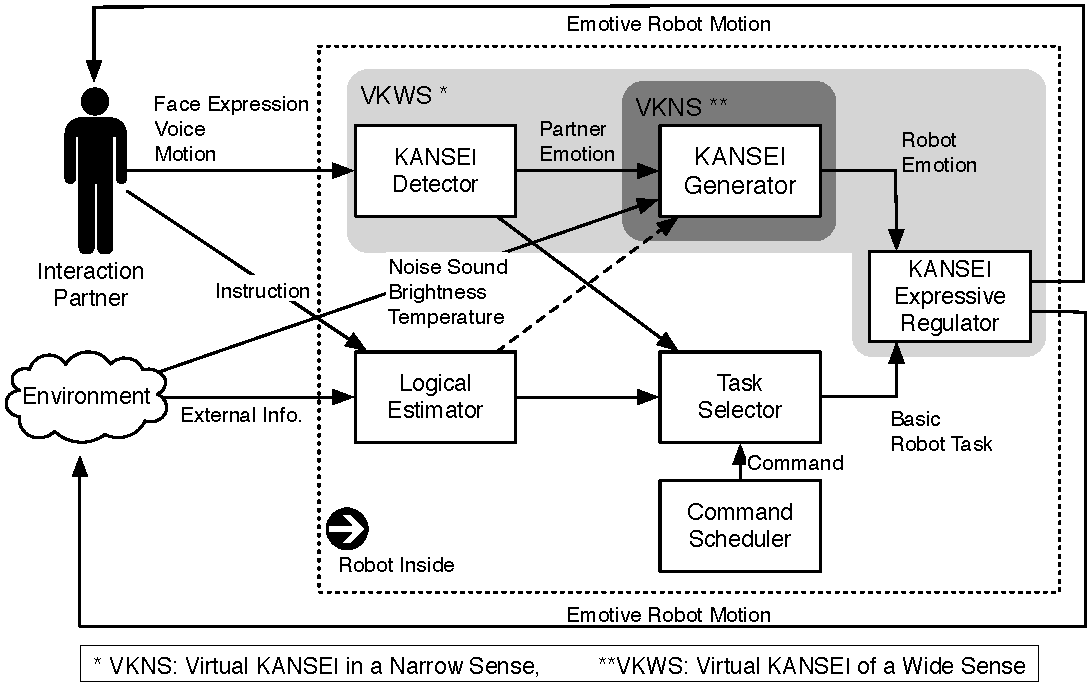
\includegraphics[width=12cm]{VKall.pdf}
  \vspace{-1mm}
  \caption{擬似感性の構成}
  \label{fig:vkall}
  \vspace{5mm}
\end{figure}

\begin{figure}[h]
  \centering
  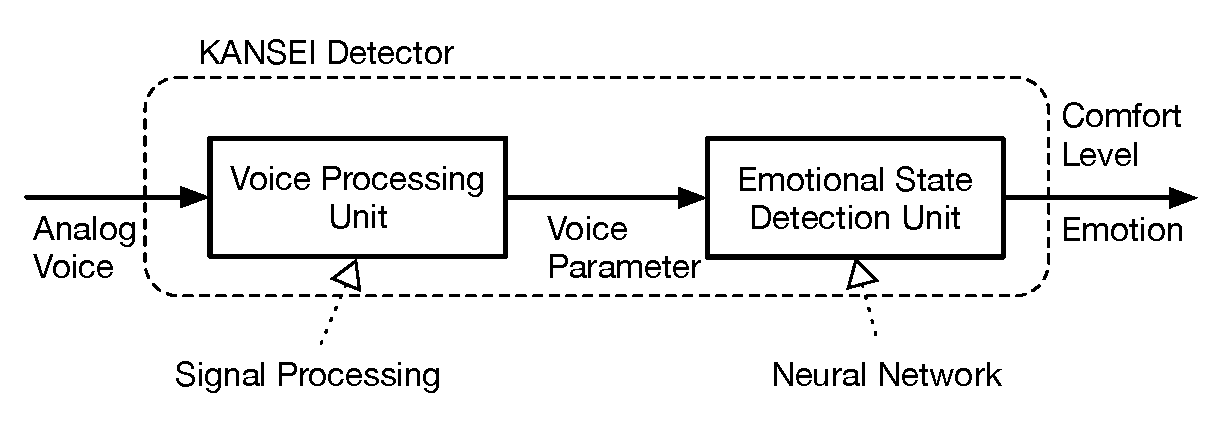
\includegraphics[width=14cm]{VoiceKANSEIDetector.pdf}
  \vspace{-1mm}
  \caption{音声からの感性同定部}
  \label{fig:VoiceKANSEIDetector}
  \vspace{5mm}
\end{figure}
% \begin{figure}[bt]
%     \centering
%     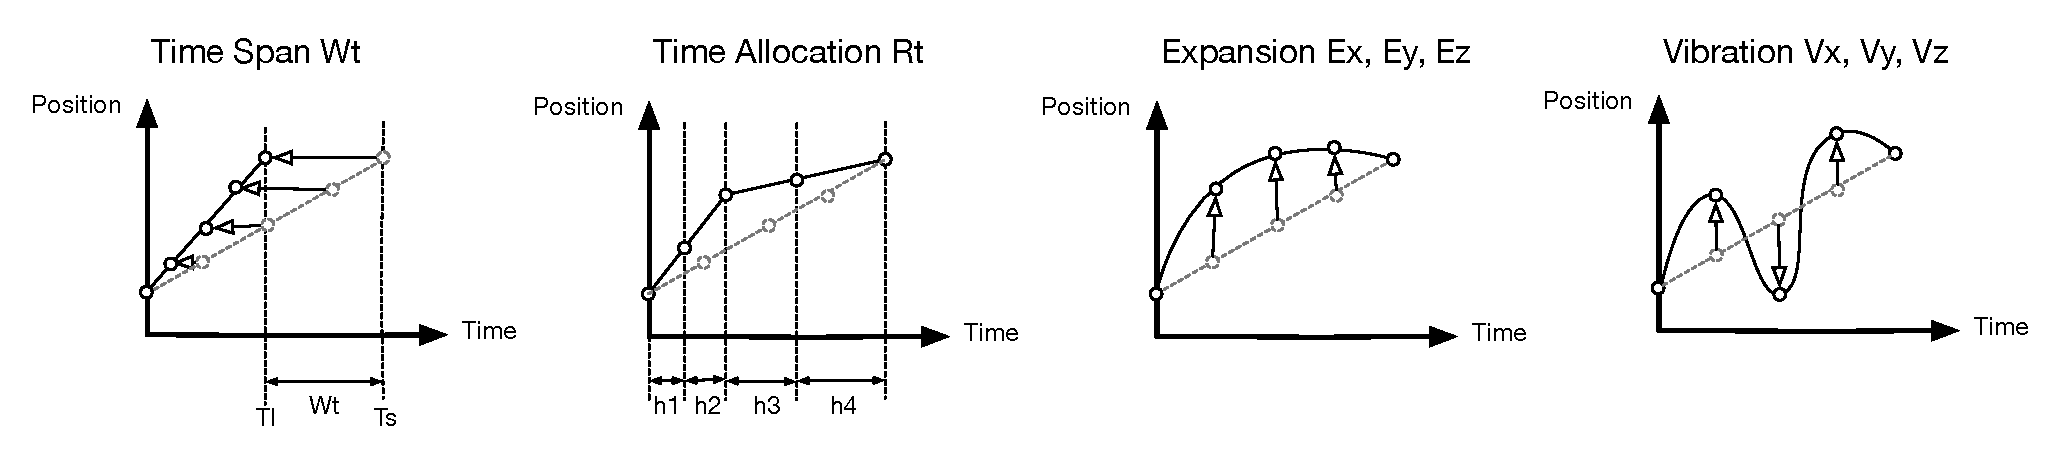
\includegraphics[width=14cm]{mp2.pdf}
%     \vspace{-1mm}
%     \caption{MMSの内部構成}
%     \label{fig:mp2}
%     \vspace{5mm}
% \end{figure}
%
\end{document} % 5章
%\include{chap6} % 6章
%\include{chap7} % 7章
\end{verbatim}
}
\end{breakbox}

なお,これらのファイルは通常の\verb+\chapter+など \LaTeX の命令でマークアップしていけば良い.
chapter1.tex や chapter2.tex,chapter3.tex 内を見れば,おおよその方法は理解できるはずである.

\subsection{付録の設定と読み込み}
付録は以下の様になっている.
\begin{breakbox}
{\small
%footnotesize
\begin{verbatim}
%%% 付録 -- 必要なければ以下を2行コメントアウト
\appendix
\documentclass[a4paper,11pt,oneside,openany]{jsbook}
\usepackage{myjlabthesisstyle}
\daigaku{青山学院大学}
\gakubu{社会情報}
\gakka{社会情報学科}
\syubetsu{卒業論文}
\labname{宮治研究室}
\chiefexaminer{宮治~~裕~~教授}

%%%%%%%%%%%%%%%%%%%%%%%%%%%%%%%%%%%%%%%
% ここから先「ここまで個人設定」の範囲に
% 各自の固有の情報を記入して下さい
%%%%%%%%%%%%%%%%%%%%%%%%%%%%%%%%%%%%%%%
\nendo{2024年度}
\teisyutsu{2024年~~1月}
\snum{38122001}
\jname{黒川~~皇輝}
\thesistitle{訪日観光客を対象とした風水害注意情報提供システム} %タイトルを記入
%\thesissubtitle{\LaTeX の利用} %サブタイトルを記入 ない場合はコメントアウト
%\SUBTtrue %サブタイトル有りの場合 ない場合は,コメントアウト
\SUBTfalse %サブタイトル無しの場合 有る場合は,コメントアウト
%%%%%%%%%% ここまで個人設定 %%%%%%%%%%%%%%

\begin{document}

\chapter{プログラムの動作方法}
本研究にて用いたプログラムについて解説する.

\section{ファイル構成}
プログラムのフォルダ内は,主に4つのファイルから構成される.

ああああいいいい

ううううええええ

これらを○○に設置し,以下の手順にそって起動する.

\section{起動方法}
まず,ウェブサーバを動かした状態にし,外部クライアント(Webブラウザから),以下のURLにアクセスする.


\section{表示の見方}
実験に利用するための,実行結果は test.log ファイルに出力されている.

このファイルは4つのカラムからなる CSV形式のファイルである.
第1列には,…

%
\end{document}

%\include{appendixB} %必要に応じて付録の数を増やす
\end{verbatim}
}
\end{breakbox}
サンプルとして 付録A(appendixA.tex)だけ読み込む様にしている.
このファイルも通常の\verb+\chapter+など通常の\LaTeX の命令でマークアップしていけば良い.
また,必要に応じて追加,コメントアウトして構わない.

\subsection{参考文献の設定と読み込み}
最後に参考文献の設定がなされている.
\begin{breakbox}
{\small
%footnotesize
\begin{verbatim}
\bibliographystyle{junsrt}
\bibliography{myrefs}
\end{verbatim}
}
\end{breakbox}
\verb+\bibliography{myrefs}+によって myrefs.bib ファイルが読み込まれている.
このファイルは \BibTeX のフォーマットにて記載されている.
詳細は3章にて記述する.
